\documentclass{beamer}
\usetheme{Madrid}
\beamertemplatenavigationsymbolsempty

\usepackage{dsfont}
\usepackage{stmaryrd}
\usepackage{colortbl}
\usepackage{hyperref}

\usepackage{amsmath}
\DeclareMathOperator*{\argmax}{argmax}
\DeclareMathOperator*{\argmin}{argmin}
\usepackage{amssymb}

\usepackage[dvipsnames, table]{xcolor}
\usepackage{textcomp}

% Packages
\usepackage[pdf]{graphviz}
\usepackage{mathrsfs}

\newcommand*\circled[1]{\tikz[baseline=-0.1cm]{
  \node[shape=circle,draw,inner sep=0.48pt] (char) {\fontsize{7}{12}\textsf{#1}};}}

\DeclareMathAlphabet{\mathcal}{OMS}{cmsy}{m}{n}
\usepackage{cancel}
\newcommand\ccancel[2][red]{\renewcommand\CancelColor{\color{#1}}\cancel{#2}}
\newcommand{\nDownarrow}{\ensuremath{\text{ }\cancel{\Downarrow}\text{ }}}
\usepackage{centernot}

\usepackage{pgfplots, pgfplotstable}
\pgfplotsset{compat=1.7}
\usepgfplotslibrary{fillbetween}
\usetikzlibrary{patterns}
\pgfmathdeclarefunction{gauss}{2}{\pgfmathparse{1/(#2*sqrt(2*pi))*exp(-((x-#1)^2)/(2*#2^2))}}
\pgfmathdeclarefunction{nil}{1}{\pgfmathparse{0.001}}

\usepackage{arydshln}
\usepackage{adjustbox}
\usepackage{enumerate}
\usepackage{enumitem}
\usepackage{tikz-cd}
\usetikzlibrary{calc}
\usepackage{amsfonts}
%\usepackage{prooftrees}
\usepackage{bussproofs}
\renewcommand{\sectionautorefname}{\S}
\renewcommand{\subsectionautorefname}{\S}
\usepackage{float}

\usepackage{tikz-3dplot}
\usetikzlibrary{3d}
\usetikzlibrary{calligraphy}
\newif\ifshowcellnumber
\showcellnumbertrue

\usepackage{algorithm}
\usepackage[noend]{algpseudocode}
\usepackage{algorithmicx}
\usepackage{sourcecodepro}
\usepackage{tikz-qtree}
\usepackage{amsthm}
\usepackage{bm}
\usetikzlibrary{bayesnet}
\usetikzlibrary{arrows}
\usepackage{subcaption}
\usetikzlibrary{backgrounds}
\usetikzlibrary{tikzmark}
\usetikzlibrary{hobby}

\usepackage{mwe}

\newcommand{\E}{\mathbb{E}}
\newcommand{\Var}{\mathrm{Var}}
\newcommand{\Cov}{\mathrm{Cov}}

\newcommand{\CompOrder}{\mathcal{O}}
\def\graphspace{\mathbf{G}}
\def\Uniform{\mbox{\rm Uniform}}
\def\Gaussian{\mbox{\rm Gaussian}}
\def\Bernoulli{\mbox{\rm Bernoulli}}
\def\Dirichlet{\mbox{\rm Dirichlet}}

\usepackage{mathtools}% superior to amsmath
\usepackage{tikz}
% Packages
\usepackage{listings}
\DeclareRobustCommand{\hlred}[1]{{\sethlcolor{pink}\hl{#1}}}
\usepackage{fontspec}

\setmonofont[Scale=0.8]{JetBrainsMono}[
Contextuals={Alternate},
Path=./font/,
Extension = .ttf,
UprightFont=*-Regular,
BoldFont=*-Bold,
ItalicFont=*-Italic,
BoldItalicFont=*-BoldItalic
]

\usepackage[skins,breakable,listings]{tcolorbox}

\lstdefinelanguage{python}{
comment=[l]{//},
commentstyle={\color{gray}\ttfamily},
emph={delegate, filter, firstOrNull, forEach, it, lazy, mapNotNull, println, repeat, assert, with, head, tail, len, return@},
numberstyle=\noncopyable,
identifierstyle=\color{black},
keywords={abstract, actual, as, as?, break, by, class, companion, continue, data, do, dynamic, else, enum, expect, false, final, for, fun, get, if, import, in, infix, interface, internal, is, null, object, open, operator, override, package, private, public, return, sealed, set, super, suspend, this, throw, true, try, catch, typealias, val, var, vararg, when, where, while, tailrec, reified, from, import, def, yield, lambda, as, in, return, else, pass},
keywordstyle={\bfseries},
morecomment=[s]{/*}{*/},
morestring=[b]",
morestring=[s]{"""*}{*"""},
ndkeywords={@Deprecated, @JvmField, @JvmName, @JvmOverloads, @JvmStatic, @JvmSynthetic, Array, Byte, Double, Float, Boolean, Int, Integer, Iterable, Long, Runnable, Short, String, int},
ndkeywordstyle={\bfseries},
sensitive=true,
stringstyle={\ttfamily},
literate={`}{{\char0}}1,
escapeinside={(*@}{@*)}
}

\lstnewenvironment{smallpy}
{\lstset{
  basicstyle=\ttfamily\lst@ifdisplaystyle\footnotesize\fi,
  language=python
}}
{}

\lstdefinelanguage{tidy}{
comment=[l]{//},
commentstyle={\color{gray}\ttfamily},
emph={|, ->, ---},
emphstyle={\color{red}},
identifierstyle=\color{black},
keywords={\|, ->, ---},
otherkeywords={|,->},
morekeywords={|,->},
keywordstyle={\color{blue}\bfseries},
morecomment=[s]{/*}{*/},
morestring=[b]",
morestring=[s]{"""*}{*"""},
ndkeywords={@Deprecated, @JvmField, @JvmName, @JvmOverloads, @JvmStatic, @JvmSynthetic, Array, Byte, Double, Float, Int, Integer, Iterable, Long, Runnable, Short, String},
ndkeywordstyle={\color{orange}\bfseries},
sensitive=true,
stringstyle={\color{green}\ttfamily},
literate={`}{{\char0}}1
}

%%%%%%%%%%%%%%%%%%%%%%%%%%%%%%%%%%%%%%%%%%%
%
% Color boxes
%
%%%%%%%%%%%%%%%%%%%%%%%%%%%%%%%%%%%%%%%%%%%

\tcbset{
  enhanced jigsaw,
  breakable,
  listing only,
%  boxsep=-1pt,
%  top=-1pt,
  bottom=0.1cm,
  right=0.5cm,
  overlay first={
    \node[black!50] (S) at (frame.south) {\Large\ding{34}};
    \draw[dashed,black!50] (frame.south west) -- (S) -- (frame.south east);
  },
  overlay middle={
    \node[black!50] (S) at (frame.south) {\Large\ding{34}};
    \draw[dashed,black!50] (frame.south west) -- (S) -- (frame.south east);
    \node[black!50] (S) at (frame.north) {\Large\ding{34}};
    \draw[dashed,black!50] (frame.north west) -- (S) -- (frame.north east);
  },
  overlay last={
    \node[black!50] (S) at (frame.north) {\Large\ding{34}};
    \draw[dashed,black!50] (frame.north west) -- (S) -- (frame.north east);
  },
  before={\par\vspace{5pt}},
  after={\par\vspace{\parskip}\noindent}
}

\definecolor{slightgray}{rgb}{0.90, 0.90, 0.90}

\usepackage{soul}
\makeatletter
\def\SOUL@hlpreamble{%
  \setul{}{3.0ex}%
  \let\SOUL@stcolor\SOUL@hlcolor%
  \SOUL@stpreamble%
}
\makeatother

\newcommand{\inline}[1]{%
  \begingroup%
  \sethlcolor{slightgray}%
  \hl{\ttfamily\footnotesize #1}%
  \endgroup
}

\newcommand{\tinline}[1]{%
  \begingroup%
  \sethlcolor{slightgray}%
  \hl{\ttfamily\tiny #1}%
  \endgroup
}

\newtcblisting{halftidyinput}[1][]{%
  left skip=0.7cm,
  left=0.35cm,
  width=6cm,
%  left=-0.01cm,
  top=-0.1cm,
  bottom=-0.35cm,
  listing options={
    language=tidy,
    basicstyle=\ttfamily\small,
%numberstyle=\footnotesize,
    showstringspaces=false,
    tabsize=2,
    breaklines=true,
    numbers=none,
    inputencoding=utf8,
    escapeinside={(*@}{@*)},
    #1
  },
  underlay unbroken and first={%
    \path[draw=none] (interior.north west) rectangle node[white]{\includegraphics[width=4mm]{../figures/tidyparse_logo.png}} ([xshift=-10mm,yshift=-7mm]interior.north west);
  }
}

\newtcblisting{wholetidyinput}[1][]{%
  left skip=0.7cm,
  left=0.35cm,
  top=0.1cm,
  middle=0mm,
  boxsep=0mm,
  listing options={
    language=tidy,
    basicstyle=\ttfamily\small,
%numberstyle=\footnotesize,
    showstringspaces=false,
    tabsize=2,
    breaklines=true,
    numbers=none,
    inputencoding=utf8,
    escapeinside={(*@}{@*)},
    #1
  },
  underlay unbroken and first={%
    \path[draw=none] (interior.north west) rectangle node[white]{\includegraphics[width=4mm]{../figures/tidyparse_logo.png}} ([xshift=-10mm,yshift=-9mm]interior.north west);
  }
}

\definecolor{A}{RGB}{6,150,104}
\definecolor{B}{RGB}{196,74,137}
\definecolor{C}{RGB}{117,237,133}
\definecolor{D}{RGB}{246,46,243}
\definecolor{E}{RGB}{89,162,12}
\definecolor{F}{RGB}{113,12,158}
\definecolor{G}{RGB}{191,205,142}
\definecolor{H}{RGB}{51,58,158}
\definecolor{I}{RGB}{244,212,3}
\definecolor{J}{RGB}{37,36,249}
\definecolor{K}{RGB}{253,165,71}
\definecolor{L}{RGB}{27,81,29}
\colorlet{LA}{A!30}
\colorlet{LB}{B!30}
\colorlet{LC}{C!30}
\colorlet{LD}{D!30}
\colorlet{LE}{E!30}
\colorlet{LF}{F!30}
\colorlet{LG}{G!30}
\colorlet{LH}{H!30}
\colorlet{LI}{I!30}
\colorlet{LJ}{J!30}
\colorlet{LK}{K!30}
\colorlet{LL}{L!30}
\newcommand{\hiliA}[1]{%
  \colorbox{LA}{$#1$}}
\newcommand{\hiliB}[1]{%
  \colorbox{LB}{$#1$}}
\newcommand{\hiliC}[1]{%
  \colorbox{LC}{$#1$}}
\newcommand{\hiliD}[1]{%
  \colorbox{LD}{$#1$}}
\newcommand{\hiliE}[1]{%
  \colorbox{LE}{$#1$}}
\newcommand{\hiliF}[1]{%
  \colorbox{LF}{$#1$}}
\newcommand{\hiliG}[1]{%
  \colorbox{LG}{$#1$}}
\newcommand{\hiliH}[1]{%
  \colorbox{LH}{$#1$}}
\newcommand{\hiliI}[1]{%
  \colorbox{LI}{$#1$}}
\newcommand{\hiliJ}[1]{%
  \colorbox{LJ}{$#1$}}
\newcommand{\hiliK}[1]{%
  \colorbox{LK}{$#1$}}
\newcommand{\hiliL}[1]{%
  \colorbox{LL}{$#1$}}
\newcommand{\highlight}[1]{%
  \colorbox{lgray}{$#1$}}
\colorlet{lred}{red!30}
\colorlet{lorange}{orange!30}
\colorlet{lgreen}{green!30}
\colorlet{lgray}{black!15}
\colorlet{dgray}{black!75}
\DeclareRobustCommand{\hlred}[1]{{\sethlcolor{lred}\hl{#1}}}
\DeclareRobustCommand{\hlorange}[1]{{\sethlcolor{lorange}\hl{#1}}}
\DeclareRobustCommand{\hlgreen}[1]{{\sethlcolor{lgreen}\hl{#1}}}
\DeclareRobustCommand{\hlgray}[1]{{\sethlcolor{lgray}\hl{#1}}}
\DeclareRobustCommand{\caret}[1]{{\sethlcolor{dgray}\textcolor{white}{\hl{#1}}}}

\usepackage{url}
\usepackage{qtree}

\usepackage{filecontents}
\usepackage{pstricks-add}
\usepackage{emoji}
\usepackage{alltt}
\usepackage{nicematrix}
\usepackage{graphicx}
\usepackage{ulem}
\usepackage{upquote}
\tikzstyle{every picture}+=[remember picture]
\usepackage{menukeys}
\pgfplotstableread[col sep=comma,]{timings_loc.csv}\loctimings
\pgfplotstableread[col sep=comma,]{timings_unloc.csv}\unloctimings

\makeatletter
\DeclareRobustCommand{\cev}[1]{%
    {\mathpalette\do@cev{#1}}%
}
\newcommand{\do@cev}[2]{%
  \vbox{\offinterlineskip
  \sbox\z@{$\m@th#1 x$}%
  \ialign{##\cr
  \hidewidth\reflectbox{$\m@th#1\vec{}\mkern4mu$}\hidewidth\cr
  \noalign{\kern-\ht\z@}
    $\m@th#1#2$\cr
  }%
  }%
}
\makeatother

\makeatletter
\DeclareRobustCommand{\pder}[1]{%
  \@ifnextchar\bgroup{\@pder{#1}}{\@pder{}{#1}}}
\newcommand{\@pder}[2]{\frac{\partial#1}{\partial#2}}
\makeatother

\newcommand{\shup}{\shortuparrow}
\newcommand{\shri}{\shortrightarrow}
\newcommand{\shur}{\shup\hspace{-5pt}\shri}

\makeatletter
\def\squigglyred{\bgroup \markoverwith{\textcolor{red}{\lower3\p@\hbox{\sixly \char58}}}\ULon}
\makeatother

\makeatletter
\def\squigglyblu{\bgroup \markoverwith{\textcolor{blue}{\lower3\p@\hbox{\sixly \char58}}}\ULon}
\makeatother

\makeatletter
\def\squigglyora{\bgroup \markoverwith{\textcolor{orange}{\lower3\p@\hbox{\sixly \char58}}}\ULon}
\makeatother

\newcommand{\err}[1]{\smash{\squigglyred{#1}{}}}
\newcommand{\erb}[1]{\smash{\squigglyblu{#1}{}}}
\newcommand{\ero}[1]{\smash{\squigglyora{#1}{}}}
\newcommand{\stirlingii}{\genfrac{\{}{\}}{0pt}{}}

%======== Arrows =========
\newcommand{\knightarrow}{
  \tikz{
    \fill (0pt,0pt) circle [radius = 1pt];
    \fill (0pt,6pt) circle [radius = 1pt];
    \fill (6pt,0pt) circle [radius = 1pt];
    \fill (6pt,6pt) circle [radius = 1pt];
    \fill (12pt,0pt) circle [radius = 1pt];
    \fill (12pt,6pt) circle [radius = 1pt];
    \fill (6pt,0pt) circle [radius = 1pt];
    \fill (12pt,0pt) circle [radius = 1pt];
    \draw [-to] (0pt,0pt) -- (12pt,6pt);
  }
}

\newcommand{\kingarrow}{
  \tikz{
    \fill (0pt,0pt) circle [radius = 1pt];
    \fill (6pt,0pt) circle [radius = 1pt];
    \fill (0pt,6pt) circle [radius = 1pt];
    \fill (6pt,6pt) circle [radius = 1pt];
    \draw [-to] (0pt,0pt) -- (6pt,6pt);
    \draw [-to] (0pt,0pt) -- (0pt,6pt);
    \draw [-to] (0pt,0pt) -- (6pt,0pt);
  }
}

\newcommand{\duparrow}{
  \tikz{
    \fill[white] (0pt,0pt) circle [radius = 1pt];
    \fill (6pt,0pt) circle [radius = 1pt];
    \fill (0pt,6pt) circle [radius = 1pt];
    \fill[white] (6pt,6pt) circle [radius = 1pt];
    \draw [-to] (6pt,0pt) -- (0pt,6pt);
  }
}

\newcommand{\drightarrow}{
  \tikz{
    \fill (0pt,0pt) circle [radius = 1pt];
    \fill (6pt,0pt) circle [radius = 1pt];
    \draw [-to] (0pt,0pt) -- (6pt,0pt);
  }
}

\newcommand{\ddiagarrow}{
  \tikz{
    \fill (0pt,0pt) circle [radius = 1pt];
    \fill (6pt,0pt) circle [radius = 1pt];
    \fill (0pt,6pt) circle [radius = 1pt];
    \fill (6pt,6pt) circle [radius = 1pt];
    \draw [-to] (0pt,0pt) -- (6pt,6pt);
  }
}

\newcommand{\knightkingarrow}{
  \tikz{
    \fill (0pt,0pt) circle [radius = 1pt];
    \fill (0pt,6pt) circle [radius = 1pt];
    \fill (6pt,0pt) circle [radius = 1pt];
    \fill (6pt,6pt) circle [radius = 1pt];
    \fill (12pt,0pt) circle [radius = 1pt];
    \fill (12pt,6pt) circle [radius = 1pt];
    \draw [-to] (0pt,0pt) -- (6pt,6pt);
    \draw [-to] (0pt,0pt) -- (0pt,6pt);
    \draw [-to] (0pt,0pt) -- (6pt,0pt);
    \draw [-to] (0pt,0pt) -- (12pt,6pt);
  }
}

%======== Arrows =========

\usetikzlibrary{decorations.pathreplacing,automata,calc,positioning,matrix,chains,fit,decorations.pathmorphing}

\usepackage{wrapfig}

\newcommand{\mkTrellis}[1]{
  \begin{tikzpicture}
    \def\dx{20pt}
    \def\dy{30pt}
    \newcounter{i}
    \stepcounter{i}
    \node[circle, draw, fill=black!30] (\arabic{i}) at (0,0){};
    \foreach [count=\i] \x in {2,...,#1}{
      \pgfmathsetmacro{\lox}{\x-1}%
      \pgfmathsetmacro{\loxt}{\x-3}%
      \foreach [count=\j] \xx in {-\lox,-\loxt,...,\lox}{
        \pgfmathsetmacro{\jj}{\j-1}%
        \stepcounter{i}
        \pgfmathsetmacro{\kk}{\xx-2}%
        \pgfmathsetmacro{\lbl}{\lox!/(\jj!*(\lox-\jj)!)}
        \ifnum\x<\kk
        \pgfmath\node[circle, draw]  (\arabic{i}) at (\xx*\dx, -\lox*\dy) {};
        \else
        \pgfmath\node[circle, draw, fill=black!30]  (\arabic{i}) at (\xx*\dx, -\lox*\dy) {};
        \fi
      }
    }
    \newcounter{z}
    \newcounter{xn}
    \newcounter{xnn}
    \pgfmathsetmacro{\maxx}{#1 - 1}
    \foreach \x in {1,...,\maxx}{
      \foreach \xx in {1,...,\x}{
        \stepcounter{z}
        \setcounter{xn}{\arabic{z}}
        \addtocounter{xn}{\x}
        \setcounter{xnn}{\arabic{xn}}
        \stepcounter{xnn}
        \draw [<-] (\arabic{z}) -- (\arabic{xn});
        \draw [<-] (\arabic{z}) -- (\arabic{xnn});
      }
    }
  \end{tikzpicture}
}

\newcommand{\dx}{20pt}
\newcommand{\dy}{30pt}
\newcounter{i}
\newcounter{z}
\newcounter{xn}
\newcounter{xnn}
\newcommand{\mkTrellisAppend}[1]{
  \begin{tikzpicture}
    \setcounter{i}{0}
    \setcounter{z}{0}
    \setcounter{xn}{0}
    \setcounter{xnn}{0}
    \stepcounter{i}
    \node[circle, draw] (\arabic{i}) at (0,0){};
    \foreach [count=\i] \x in {2,...,#1}{
      \pgfmathsetmacro{\lox}{\x-1}%
      \pgfmathsetmacro{\loxt}{\x-3}%
      \foreach [count=\j] \xx in {-\lox,-\loxt,...,\lox}{
        \pgfmathsetmacro{\jj}{\j-1}%
        \stepcounter{i}
        \pgfmathsetmacro{\kk}{\xx+2}%
        \pgfmathsetmacro{\lbl}{\lox!/(\jj!*(\lox-\jj)!)}
        \ifnum\x>\kk
        \pgfmath\node[circle, draw, fill=black!30]  (\arabic{i}) at (\xx*\dx, -\lox*\dy) {};
        \else
        \pgfmath\node[circle, draw]  (\arabic{i}) at (\xx*\dx, -\lox*\dy) {};
        \fi
      }
    }
    \pgfmathsetmacro{\maxx}{#1 - 1}
    \foreach \x in {1,...,\maxx}{
      \foreach \xx in {1,...,\x}{
        \stepcounter{z}
        \setcounter{xn}{\arabic{z}}
        \addtocounter{xn}{\x}
        \setcounter{xnn}{\arabic{xn}}
        \stepcounter{xnn}
        \draw [<-] (\arabic{z}) -- (\arabic{xn});
        \draw [<-] (\arabic{z}) -- (\arabic{xnn});
      }
    }
  \end{tikzpicture}
}

\newcommand{\mkTrellisInsert}[1]{
  \begin{tikzpicture}
    \setcounter{i}{0}
    \setcounter{z}{0}
    \setcounter{xn}{0}
    \setcounter{xnn}{0}
    \stepcounter{i}
    \node[circle, draw] (\arabic{i}) at (0,0){};
    \foreach [count=\i] \x in {2,...,#1}{
      \pgfmathsetmacro{\lox}{\x-1}%
      \pgfmathsetmacro{\loxt}{\x-3}%
      \foreach [count=\j] \xx in {-\lox,-\loxt,...,\lox}{
        \pgfmathsetmacro{\jj}{\j-1}%
        \stepcounter{i}
        \pgfmathsetmacro{\mp}{\xx+#1}%
        \pgfmathsetmacro{\mq}{\xx+\x}%
        \pgfmathsetmacro{\lbl}{\lox!/(\jj!*(\lox-\jj)!)}
        \ifnum\x>\mp
        \pgfmath\node[circle, draw, fill=black!30]  (\arabic{i}) at (\xx*\dx, -\lox*\dy) {};
        \else
        \ifnum#1<\mq
        \pgfmath\node[circle, draw, fill=black!30]  (\arabic{i}) at (\xx*\dx, -\lox*\dy) {};
        \else
        \pgfmath\node[circle, draw]  (\arabic{i}) at (\xx*\dx, -\lox*\dy) {};
        \fi
        \fi

      }
    }
    \pgfmathsetmacro{\maxx}{#1 - 1}
    \foreach \x in {1,...,\maxx}{
      \foreach \xx in {1,...,\x}{
        \stepcounter{z}
        \setcounter{xn}{\arabic{z}}
        \addtocounter{xn}{\x}
        \setcounter{xnn}{\arabic{xn}}
        \stepcounter{xnn}
        \draw [<-] (\arabic{z}) -- (\arabic{xn});
        \draw [<-] (\arabic{z}) -- (\arabic{xnn});
      }
    }
  \end{tikzpicture}
}

\usetikzlibrary{automata, positioning, arrows}

\newcommand{\nobarfrac}{\genfrac{}{}{0pt}{}}
\pgfplotstableread[col sep=comma,]{timings_loc.csv}\loctimings
\pgfplotstableread[col sep=comma,]{timings_unloc.csv}\unloctimings
\pgfplotstableread[col sep=comma,]{natural_errors.csv}\naturalerrors
\pgfplotstableread[col sep=comma,]{synthetic_errors.csv}\syntheticerrors

\usepackage[all,pdf]{xy}

\newcommand{\bs}{\blacksquare}
\newcommand{\ws}{\square}

\usepackage{multicol}
\usetikzlibrary{shapes.geometric, arrows}

\tikzstyle{startstop} = [rectangle, rounded corners,
minimum width=3cm,
minimum height=1cm,
thick,
text centered,
draw=none,
]

\tikzstyle{plain} = [
rectangle,
rounded corners,
minimum width=3.5cm,
minimum height=1cm,
thick,
text centered,
draw=black
]

\tikzstyle{io} = [trapezium,
trapezium stretches=true, % A later addition
thick,
trapezium left angle=70,
trapezium right angle=110,
minimum width=3cm,
minimum height=1cm, text centered,
draw=black, fill=blue!30]

\tikzstyle{io2} = [trapezium,
trapezium stretches=true, % A later addition
thick,
trapezium left angle=70,
trapezium right angle=110,
minimum width=3cm,
minimum height=1cm, text centered,
draw=black, fill=black!30]

\tikzstyle{process} = [rectangle,
minimum width=3.5cm,
minimum height=1cm,
thick,
text centered,
text width=4cm,
draw=black,
fill=orange!30]

\tikzstyle{decision} = [diamond,
minimum width=2.5cm,
minimum height=0.5cm,
thick,
text centered,
draw=black,
fill=green!30]
\tikzstyle{arrow} = [->,thick]

%\usetikzlibrary{external}
%\tikzexternalize[prefix=figures/]
\definecolor{green}{RGB}{0,128,0}
\definecolor{darkgray176}{RGB}{176,176,176}
\definecolor{darkviolet1270255}{RGB}{127,0,255}
\definecolor{deepskyblue3176236}{RGB}{3,176,236}
\definecolor{dodgerblue45123246}{RGB}{45,123,246}
\definecolor{lightgray204}{RGB}{204,204,204}
\definecolor{royalblue8762253}{RGB}{87,62,253}

\usepackage{sankey}

\usepackage{pgf-soroban}
\usetikzlibrary{shapes.geometric,calc,decorations.text,bayesnet,arrows,backgrounds}
\usepackage{circledsteps}
\usepackage{epigraph}
\usepackage{array}
\setmonofont{JetBrains Mono}[
  Contextuals = Alternate,
  Ligatures = TeX,
]
\lstset{
  basicstyle = \ttfamily,
  columns = flexible,
}
\makeatletter
\renewcommand*\verbatim@nolig@list{}
\makeatother
\usepackage{pmboxdraw}
\usetikzlibrary{cd}
\usepackage{pifont}
\newcommand{\cmark}{\ding{51}}%
\newcommand{\xmark}{\ding{55}}%

\setbeamertemplate{footline}
{
  \leavevmode%
  \hbox{%
    \begin{beamercolorbox}[wd=.25\paperwidth,ht=2.25ex,dp=1ex,center]{author in head/foot}%
      \usebeamerfont{author in head/foot}\insertshortauthor{}{~~(\insertshortinstitute)}
    \end{beamercolorbox}%
    \begin{beamercolorbox}[wd=.5\paperwidth,ht=2.25ex,dp=1ex,center]{title in head/foot}%
      \usebeamerfont{title in head/foot}\insertshorttitle
    \end{beamercolorbox}%
    \begin{beamercolorbox}[wd=.3\paperwidth,ht=2.25ex,dp=1ex,right]{date in head/foot}%
      \usebeamerfont{date in head/foot}\insertshortdate{}\hspace*{2em}
      \insertframenumber{} / \inserttotalframenumber\hspace*{2ex}
    \end{beamercolorbox}}%
  \vskip0pt%
}
\makeatother

\makeatletter
\let\HL\hl
\renewcommand\hl{%
  \let\set@color\beamerorig@set@color
  \let\reset@color\beamerorig@reset@color
  \HL}
\makeatother

\newcommand{\ddd}{\Ddots}
\newcommand{\vdd}{\Vdots}
\newcommand{\cdd}{\Cdots}
\newcommand{\lds}{\ldots}
\newcommand{\vno}{\varnothing}
\newcommand{\ts}[1]{\textsuperscript{#1}}
\newcommand{\non}{1\ts{st}}
\newcommand{\ntw}{2\ts{nd}}
\newcommand{\nth}{3\ts{rd}}
\newcommand{\nfo}{4\ts{th}}
\newcommand{\nfi}{5\ts{th}}
\newcommand{\nsi}{6\ts{th}}
\newcommand{\nse}{7\ts{th}}
\newcommand{\vs}[1]{\sigma_{#1}^{\shur}}
\newcommand{\rcr}{\rowcolor{black!15}}
\newcommand{\rcw}{\rowcolor{white}}
\newcommand{\pcd}{\cdot}
\newcommand{\pcp}{\phantom\cdot}
\newcommand{\ppp}{\phantom{\nse}}
\newcommand{\hole}{\underline{\hspace{0.25cm}}}

\title[Syntax Repair as Language Intersection]{Syntax Repair as Language Intersection}
\titlegraphic{\includegraphics[width=0.2\textwidth]{../figures/tidyparse_logo.png}}
\author[Considine, Guo, Si]{\textbf{Breandan Considine}, Jin Guo, Xujie Si}
\institute[McGill]{
  McGill University, Mila IQIA\\
  \medskip
  \textit{bre@ndan.co}
}
\date{\today}

\begin{document}
\begin{frame}
  \titlepage
\end{frame}

\begin{frame}{Overview}
  \tableofcontents
\end{frame}

\begin{frame}[fragile]{Can you spot the error?}
  \begin{center}
    \begin{tabular}{|m{5.5cm}|m{5.5cm}|}
      \hline \rule{0pt}{2.5ex}\textbf{Original code}\rule[-1ex]{0pt}{2ex} &  \rule{0pt}{2.5ex}\textbf{Human repair}\rule[-1ex]{0pt}{2ex} \\\hline
      \begin{lstlisting}[escapechar=!, basicstyle=\linespread{1.3}\ttfamily\footnotesize]

  newlist = []
  i = set([5, 3, 1)]
  z = set([5, 0, 4)]


      \end{lstlisting} & \begin{lstlisting}[escapechar=!, basicstyle=\linespread{1.3}\ttfamily\footnotesize]

      \end{lstlisting} \\\hline
    \end{tabular}
  \end{center}
\end{frame}

\begin{frame}[fragile]{Can you spot the error?}
  \begin{center}
    \begin{tabular}{|m{5.5cm}|m{5.5cm}|}
      \hline \rule{0pt}{2.5ex}\textbf{Original code}\rule[-1ex]{0pt}{2ex} &  \rule{0pt}{2.5ex}\textbf{Human repair}\rule[-1ex]{0pt}{2ex} \\\hline
      \begin{lstlisting}[escapechar=!, basicstyle=\linespread{1.3}\ttfamily\footnotesize]

  newlist = []
  i = set([5, 3, 1)]
  z = set([5, 0, 4)]

      \end{lstlisting} & \begin{lstlisting}[escapechar=!, basicstyle=\linespread{1.3}\ttfamily\footnotesize]

  newlist = []
  i = set([5, 3, 1!\hlorange{])}!
  z = set([5, 0, 4!\hlorange{])}!

      \end{lstlisting} \\\hline
    \end{tabular}
  \end{center}
\end{frame}

\begin{frame}[fragile]{Can you spot the error?}
  \begin{center}
    \begin{tabular}{|m{5.5cm}|m{5.5cm}|}
      \hline \rule{0pt}{2.5ex}\textbf{Original code}\rule[-1ex]{0pt}{2ex} &  \rule{0pt}{2.5ex}\textbf{Human repair}\rule[-1ex]{0pt}{2ex} \\\hline
      \begin{lstlisting}[escapechar=!, basicstyle=\linespread{1.3}\ttfamily\footnotesize]

  def average(values):
    if values == (1,2,3):
      return (1+2+3)/3
    else if values == (-3,2):
      return (-3+2+8-1)/4

      \end{lstlisting} & \begin{lstlisting}[escapechar=!, basicstyle=\linespread{1.3}\ttfamily\footnotesize]

      \end{lstlisting} \\\hline
    \end{tabular}
  \end{center}
\end{frame}

\begin{frame}[fragile]{Can you spot the error?}
  \begin{center}
    \begin{tabular}{|m{5.5cm}|m{5.5cm}|}
      \hline \rule{0pt}{2.5ex}\textbf{Original code}\rule[-1ex]{0pt}{2ex} &  \rule{0pt}{2.5ex}\textbf{Human repair}\rule[-1ex]{0pt}{2ex} \\\hline
      \begin{lstlisting}[escapechar=!, basicstyle=\linespread{1.3}\ttfamily\footnotesize]

  def average(values):
    if values == (1,2,3):
      return (1+2+3)/3
    !\hlorange{else}! !\hlred{if}! values == (-3,2):
      return (-3+2+8-1)/4

      \end{lstlisting} & \begin{lstlisting}[escapechar=!, basicstyle=\linespread{1.3}\ttfamily\footnotesize]

  def average(values):
    if values == (1,2,3):
      return (1+2+3)/3
    !\hlorange{elif}! values == (-3,2):
      return (-3+2+8-1)/4

      \end{lstlisting} \\\hline
    \end{tabular}
  \end{center}
\end{frame}

\begin{frame}[fragile]{Can you spot the error?}
  \begin{center}
    \begin{tabular}{|m{5.5cm}|m{5.5cm}|}
      \hline \rule{0pt}{2.5ex}\textbf{Original code}\rule[-1ex]{0pt}{2ex} &  \rule{0pt}{2.5ex}\textbf{Human repair}\rule[-1ex]{0pt}{2ex} \\\hline
      \begin{lstlisting}[escapechar=!, basicstyle=\linespread{1.3}\ttfamily\footnotesize]

  import Global from Global
  globalObj = Global()
  print(str(globalObj.Test()))

      \end{lstlisting} & \begin{lstlisting}[escapechar=!, basicstyle=\linespread{1.3}\ttfamily\footnotesize]

      \end{lstlisting} \\\hline
    \end{tabular}
  \end{center}
\end{frame}

\begin{frame}[fragile]{Can you spot the error?}
  \begin{center}
    \begin{tabular}{|m{5.5cm}|m{5.5cm}|}
      \hline \rule{0pt}{2.5ex}\textbf{Original code}\rule[-1ex]{0pt}{2ex} &  \rule{0pt}{2.5ex}\textbf{Human repair}\rule[-1ex]{0pt}{2ex} \\\hline
      \begin{lstlisting}[escapechar=!, basicstyle=\linespread{1.3}\ttfamily\footnotesize]

  !\hlorange{import}! Global !\hlorange{from}! Global
  globalObj = Global()
  print(str(globalObj.Test()))

      \end{lstlisting} & \begin{lstlisting}[escapechar=!, basicstyle=\linespread{1.3}\ttfamily\footnotesize]

  !\hlorange{from}! Global !\hlorange{import}! Global
  globalObj = Global()
  print(str(globalObj.Test()))

      \end{lstlisting} \\\hline
    \end{tabular}
  \end{center}
\end{frame}

%\begin{frame}[fragile]{Can you spot the error?}
%  \begin{center}
%    \begin{tabular}{|m{5.5cm}|m{5.5cm}|}
%      \hline \rule{0pt}{2.5ex}\textbf{Original code}\rule[-1ex]{0pt}{2ex} &  \rule{0pt}{2.5ex}\textbf{Human repair}\rule[-1ex]{0pt}{2ex} \\\hline
%      \begin{lstlisting}[escapechar=!, basicstyle=\linespread{1.3}\ttfamily\footnotesize]
%
%   try:
%     something()
%   catch AttributeError:
%     pass
%
%      \end{lstlisting} & \begin{lstlisting}[escapechar=!, basicstyle=\linespread{1.3}\ttfamily\footnotesize]
%
%      \end{lstlisting} \\\hline
%    \end{tabular}
%  \end{center}
%\end{frame}
%
%\begin{frame}[fragile]{Can you spot the error?}
%  \begin{center}
%    \begin{tabular}{|m{5.5cm}|m{5.5cm}|}
%      \hline \rule{0pt}{2.5ex}\textbf{Original code}\rule[-1ex]{0pt}{2ex} &  \rule{0pt}{2.5ex}\textbf{Human repair}\rule[-1ex]{0pt}{2ex} \\\hline
%      \begin{lstlisting}[escapechar=!, basicstyle=\linespread{1.3}\ttfamily\footnotesize]
%
%   try:
%     something()
%   !\hlorange{catch}! AttributeError:
%     pass
%
%      \end{lstlisting} & \begin{lstlisting}[escapechar=!, basicstyle=\linespread{1.3}\ttfamily\footnotesize]
%
%   try:
%     something()
%   !\hlorange{except}! AttributeError:
%     pass
%
%      \end{lstlisting} \\\hline
%    \end{tabular}
%  \end{center}
%\end{frame}

\begin{frame}[t,fragile]{How many repairs could there possibly be?}
  Consider the following Python snippet, which contains a small syntax error:\\

  \begin{lstlisting}[escapechar=!, basicstyle=\linespread{1.3}\ttfamily\footnotesize]
    def prepend(i, k, L=[])
      n and [prepend(i - 1, k, [b] + L) for b in range(k)]
  \end{lstlisting}
\end{frame}

\begin{frame}[t,fragile]{How many repairs could there possibly be?}
  Consider the following Python snippet, which contains a small syntax error:\\

  \begin{lstlisting}[escapechar=!, basicstyle=\linespread{1.3}\ttfamily\footnotesize]
    def prepend(i, k, L=[])
      n and [prepend(i - 1, k, [b] + L) for b in range(k)]
  \end{lstlisting}

  It can be fixed by appending a colon after the function signature, yielding:\\

    \begin{lstlisting}[escapechar=!, basicstyle=\linespread{1.3}\ttfamily\footnotesize]
    def prepend(i, k, L=[])!\hlgreen{:}!
      n and [prepend(i - 1, k, [b] + L) for b in range(k)]
    \end{lstlisting}
\end{frame}

\begin{frame}[t,fragile]{How many repairs could there possibly be?}
  Consider the following Python snippet, which contains a small syntax error:\\

  \begin{lstlisting}[escapechar=!, basicstyle=\linespread{1.3}\ttfamily\footnotesize]
    def prepend(i, k, L=[])
      n and [prepend(i - 1, k, [b] + L) for b in range(k)]
  \end{lstlisting}

  It can be fixed by appending a colon after the function signature, yielding:\\

  \begin{lstlisting}[escapechar=!, basicstyle=\linespread{1.3}\ttfamily\footnotesize]
    def prepend(i, k, L=[])!\hlgreen{:}!
      n and [prepend(i - 1, k, [b] + L) for b in range(k)]
  \end{lstlisting}

  \vspace{0.5cm}

  \normalsize Let us consider a slightly more ambiguous error: \footnotesize{\texttt{v = df.iloc(5:, 2:)}}. \normalsize Assuming an alphabet of just a hundred lexical tokens, this statement has millions of two-token edits, yet only six are accepted by the Python parser:
\end{frame}

\begin{frame}[t,fragile]{How many repairs could there possibly be?}
  Consider the following Python snippet, which contains a small syntax error:\\

  \begin{lstlisting}[escapechar=!, basicstyle=\linespread{1.3}\ttfamily\footnotesize]
    def prepend(i, k, L=[])
      n and [prepend(i - 1, k, [b] + L) for b in range(k)]
  \end{lstlisting}

  It can be fixed by appending a colon after the function signature, yielding:\\

  \begin{lstlisting}[escapechar=!, basicstyle=\linespread{1.3}\ttfamily\footnotesize]
    def prepend(i, k, L=[])!\hlgreen{:}!
      n and [prepend(i - 1, k, [b] + L) for b in range(k)]
  \end{lstlisting}

  \vspace{0.5cm}

  \normalsize Let us consider a slightly more ambiguous error: \footnotesize{\texttt{v = df.iloc(5:, 2:)}}. \normalsize Assuming an alphabet of just a hundred lexical tokens, this statement has millions of two-token edits, yet only six are accepted by the Python parser:

    \scriptsize
    \begin{figure}[h!]
      \noindent\begin{tabular}{@{}l@{\hspace{10pt}}l@{\hspace{10pt}}l@{}}
      (1) \texttt{v = df.iloc(5\hlred{:}, 2\hlorange{,})} & (3) \texttt{v = df.iloc(5\hlgreen{[}:, 2:\hlgreen{]})} & (5) \texttt{v = df.iloc\hlorange{[}5:, 2:\hlorange{]}} \\\\
      (2) \texttt{v = df.iloc(5\hlorange{)}, 2\hlorange{(})} & (4) \texttt{v = df.iloc(5\hlred{:}, 2\hlred{:})} & (6) \texttt{v = df.iloc(5\hlgreen{[}:, 2\hlorange{]})} \\
      \end{tabular}
    \end{figure}
\end{frame}

\begin{frame}[fragile]{On the virtues of pragmatism}
  \textbf{Pragmatism}: \textit{a reasonable and logical way of solving problems that is based on dealing with specific situations instead of abstract theories.}\newline\\
  \begin{itemize}
    \item Often framed as a compromise, \textit{``Let's be pragmatic...''}
    \item Pragmatism is a principled approach to problem solving.
    \item Taken seriously, pragmatism is difficult because it requires modeling the needs of multiple stakeholders and balancing competing interests.
    \item Putting it into practice requires knowing your customer, understanding their workflow, considering the most appropriate solution out of a set of possible alternatives.
  \end{itemize}
    \setlength{\epigraphwidth}{0.97\textwidth}
    \epigraph{``\textit{What is the use of studying philosophy if all that it does for you is to enable you to talk about some abstruse questions of logic and does not improve your thinking about the important questions of everyday life?}''}{Ludwig Wittgenstein, 1889–1951}
\end{frame}

\begin{frame}[fragile]{On the virtues of pragmatism}
  \begin{columns}[T]
    \begin{column}{0.9\textwidth}
      \begin{itemize}
        \item Pioneered in the 19th century by Peirce, James, Dewey, et al.
        \item Wittgenstein was a pragmatist, early work on language games.
        \item Pragmatism is a philosophy of language that emphasizes the role of intent in human communication.
        \item Language is a tool for communication, \\not just a arbitrary set of rules.
        \item Must actively imagine the mindset of\\ the speaker, not just the literal\\meaning of their words.
        \item Language is a bit like a game whose goal \\is to understand the speaker's intent.
        \item Assume a proficient speaker, who is trying \\to communicate something meaningful.
      \end{itemize}
    \end{column}
    \begin{column}{0.6\textwidth}
      \vspace*{2cm}
      \hspace*{-3cm}
      \includegraphics[width=1.7cm]{../figures/photo_pierce.png}
      \includegraphics[width=2.6cm]{../figures/photo_wittgenstein.png}
    \end{column}
  \end{columns}
\end{frame}

%\begin{frame}[fragile]{Common sources of syntax errors}
%  \begin{itemize}
%    \item Reading impairments (e.g., dyslexia, dysgraphia)
%    \item Motor impairments (e.g., tremors, Parkinson's)
%    \item Speech impediments (e.g., stuttering, apraxia, Tourette's)
%    \item Visual impairments (e.g., poor eyesight, blindness)
%    \item Language barriers (e.g., foreign and non-native speakers)
%    \item Inexperience (e.g., novice programmers)
%    \item Distraction (e.g., multitasking, fatigue, stress)
%    \item Time pressure (e.g., deadlines, interview coding)
%    \item Inattention (e.g., typographic mistakes, boredom, apathy)
%    \item Lack of feedback (e.g., no syntax highlighting or IDE)
%  \end{itemize}
%\end{frame}

\begin{frame}{From Error-Correcting Codes to Correcting Coding Errors}
  \begin{itemize}
    \item Error-correcting codes are a well-studied topic in information theory used to detect and correct errors in data transmission.
    \item Introduces parity bits to detect and correct transmission errors assuming a certain noise model (e.g., Hamming distance).
    \item Like ECCs, we also assume a certain noise model (Levenshtein distance) and error tolerance (n-lexical tokens).
    \item Instead of injecting parity bits, we use the grammar and mutual information between tokens to detect and correct errors.
    \item Unlike ECCs, we do not assume a unique solution, but a set of admissible solutions ranked by statistical likliehood.
    \end{itemize}
  \setlength{\epigraphwidth}{0.97\textwidth}
  \epigraph{``\textit{Damn it, if the machine can detect an error, why can't it\\\phantom{``}locate the position of the error and correct it?'}''}{Richard Hamming, 1915-1998}
\end{frame}

\begin{frame}[fragile]{Syntax repair as a language game}
  \begin{itemize}
    \item Imagine a game between two players, \textit{Editor} and \textit{Author}.
    \item They both see the same grammar, $\mathcal{G}$ and invalid string $\err\sigma \notin \mathcal{L}(\mathcal{G})$.
    % Both players move simultaneously after a short period of deliberation. As soon as Player A repairs $\err\sigma$, Player B must move immediately.
    \item Author moves by modifying $\err\sigma$ to produce a valid string, $\sigma \in \mathcal{L}(\mathcal{G})$.
    \item Editor moves continuously, sampling a set $\tilde{\bm\sigma} \subseteq \mathcal{L}(\mathcal{G})$.
    \item As soon as Author repairs $\err\sigma$, the turn immediately ends.
    \item Neither player sees the other's move(s) before making their own.
    \item If Editor anticipates Author's move, i.e., $\sigma \in \tilde{\bm\sigma}$, they both win.
    \item If Author surprises Editor with a valid move, i.e., $\sigma \notin \tilde{\bm\sigma}$, Author wins.
    \item We may consider a refinement where Editor wins in proportion to the time taken to anticipate Author's move.
  \end{itemize}
\end{frame}

  \begin{frame}[fragile]{Can you spot the error?}
  \begin{center}
  \begin{tabular}{|m{5.5cm}|m{5.5cm}|}
  \hline \rule{0pt}{2.5ex}\textbf{Original code}\rule[-1ex]{0pt}{2ex} &  \rule{0pt}{2.5ex}\textbf{Valid repairs}\rule[-1ex]{0pt}{2ex} \\\hline
  \begin{lstlisting}[escapechar=!, basicstyle=\linespread{1.3}\ttfamily\footnotesize]

  !\phantom{( ) )}

  \end{lstlisting} & \begin{lstlisting}[escapechar=!, basicstyle=\linespread{1.3}\ttfamily\footnotesize]

  \end{lstlisting} \\\hline
  \end{tabular}
  \end{center}
  \end{frame}

  \begin{frame}[fragile]{Can you spot the error?}
  \begin{center}
  \begin{tabular}{|m{5.5cm}|m{5.5cm}|}
  \hline \rule{0pt}{2.5ex}\textbf{Original code}\rule[-1ex]{0pt}{2ex} &  \rule{0pt}{2.5ex}\textbf{Valid repairs}\rule[-1ex]{0pt}{2ex} \\\hline
  \begin{lstlisting}[escapechar=!, basicstyle=\linespread{1.3}\ttfamily\footnotesize]

  ( ) )

  \end{lstlisting} & \begin{lstlisting}[escapechar=!, basicstyle=\linespread{1.3}\ttfamily\footnotesize]

  \end{lstlisting} \\\hline
  \end{tabular}
  \end{center}
  \end{frame}

  \begin{frame}[fragile]{Can you spot the error?}
  \begin{center}
  \begin{tabular}{|m{5.5cm}|m{5.5cm}|}
  \hline \rule{0pt}{2.5ex}\textbf{Original code}\rule[-1ex]{0pt}{2ex} &  \rule{0pt}{2.5ex}\textbf{Valid repairs}\rule[-1ex]{0pt}{2ex} \\\hline
  \begin{lstlisting}[escapechar=!, basicstyle=\linespread{1.3}\ttfamily\footnotesize]

  ( ) )

  \end{lstlisting} & \begin{lstlisting}[escapechar=!, basicstyle=\linespread{1.3}\ttfamily\footnotesize]

  ( )

  \end{lstlisting} \\\hline
  \end{tabular}
  \end{center}
  \end{frame}

  \begin{frame}[fragile]{Can you spot the error?}
  \begin{center}
  \begin{tabular}{|m{5.5cm}|m{5.5cm}|}
  \hline \rule{0pt}{2.5ex}\textbf{Original code}\rule[-1ex]{0pt}{2ex} &  \rule{0pt}{2.5ex}\textbf{Valid repairs}\rule[-1ex]{0pt}{2ex} \\\hline
  \begin{lstlisting}[escapechar=!, basicstyle=\linespread{1.3}\ttfamily\footnotesize]

  ( ) )

  \end{lstlisting} & \begin{lstlisting}[escapechar=!, basicstyle=\linespread{1.3}\ttfamily\footnotesize]

  ( )
  ( ) ( )

  \end{lstlisting} \\\hline
  \end{tabular}
  \end{center}
  \end{frame}

  \begin{frame}[fragile]{Can you spot the error?}
  \begin{center}
  \begin{tabular}{|m{5.5cm}|m{5.5cm}|}
  \hline \rule{0pt}{2.5ex}\textbf{Original code}\rule[-1ex]{0pt}{2ex} &  \rule{0pt}{2.5ex}\textbf{Valid repairs}\rule[-1ex]{0pt}{2ex} \\\hline
  \begin{lstlisting}[escapechar=!, basicstyle=\linespread{1.3}\ttfamily\footnotesize]

  ( ) )

  \end{lstlisting} & \begin{lstlisting}[escapechar=!, basicstyle=\linespread{1.3}\ttfamily\footnotesize]

  ( )
  ( ) ( )
  ( ( ) )

  \end{lstlisting} \\\hline
  \end{tabular}
  \end{center}
  \end{frame}

\begin{frame}[fragile]{Problem Statement: Validity and naturalness}
  Syntax repair can be treated as a language intersection problem between a context-free language (CFL) and a regular language.

  \begin{definition}[Reachable edits]
    Given a CFL, $\ell$, and an invalid string, $\err{\sigma}: \ell^\complement$, find every valid string reachable within $d$ edits of $\err{\sigma}$, i.e., letting $\Delta$ be the Levenshtein metric and $L(\err\sigma, d) = \{\sigma' \mid \Delta(\err{\sigma}, \sigma') \leq d\}$ be the edit ball, we seek $A = L(\err\sigma, d) \cap \ell$.
  \end{definition}

  \begin{definition}[Ranked repair]
  Given a finite language $A = L(\err\sigma, d) \cap \ell$ and a probabilistic language model $\text{P}_\theta: \Sigma^* \rightarrow [0, 1] \subset \mathbb{R}$, the ranked repair problem is to find the top-$k$ maximum likelihood repairs under the language model. That is,
  \begin{equation}
    R(A, P_\theta) = \argmax_{\bm{\sigma} \subseteq A, |\bm{\sigma}| \leq k} \sum_{\sigma \in \bm{\sigma}}\text{P}_\theta(\sigma)
  \end{equation}
    \end{definition}
%  To solve this problem, we will first pose a simpler problem that only considers localized edits, then turn our attention back to BCFLR.
%
%  \begin{definition}[Porous completion]
%    Let $\underline\Sigma \coloneqq \Sigma \cup \{\hole\}$, where \hole denotes a hole. We denote $\sqsubseteq: \Sigma^n \times \underline\Sigma^n$ as the relation $\{\langle\sigma', \sigma\rangle \mid \sigma_i \in \Sigma \implies \sigma_i' = \sigma_i\}$ and the set of all inhabitants $\{\sigma' \mid \sigma' \sqsubseteq \sigma\}$ as $\text{H}(\sigma)$. Given a \textit{porous string}, $\sigma: \underline\Sigma^*$ we seek all syntactically admissible inhabitants, i.e., $A(\sigma)\coloneqq\text{H}(\sigma)\cap\ell$.
%  \end{definition}
\end{frame}

\begin{frame}[fragile]{Problem Statement: Temporal constraints}
  Find every syntactically admissible edit $\{\sigma' \in \ell \mid \Delta(\err{\sigma}, \sigma') \leq d\}$, ranked by a probability metric $P_\theta$, and return them in a reasonable amount of time.

  \begin{definition}[Linear convergence]\label{def:linear-convergence}
  Given a finite CFL, $\ell$, we want a generating function, $\bm{\varphi}: \mathbb{N}_{<|\ell|} \rightarrow 2^\ell$, that converges linearly in expectation, i.e., $\mathbb{E}_{i \in [1, n]}|\bm{\varphi}(i)| \propto n$.
  \end{definition}

  \begin{center}
    \resizebox{0.42\textwidth}{!}{
      \def\secondcirclepath{(1.15,0) coordinate (e) circle (2cm)}
      \begin{tikzpicture}[
        dot/.style = {circle, inner sep=0pt, minimum size=1mm, fill,
        node contents={}}
      ]
        \def\firstcircle{(-2.1,0) coordinate (a) circle (2.4cm)}
        \def\firstcirclea{(-2.1,0) coordinate (b) circle (0.6cm)}
        \def\firstcircleb{(-2.1,0) coordinate (c) circle (1.2cm)}
        \def\firstcirclec{(-2.1,0) coordinate (d) circle (1.8cm)}
        \def\secondcircle{(1.2,0) coordinate (e) circle (1.5cm)}

        \begin{scope}
          \clip[decorate, decoration={snake, amplitude=0.6mm, segment length=5.01mm}] \secondcirclepath;
          \fill[black!15] \firstcircle;
        \end{scope}

        \draw \firstcircle node[dot,label=$\err{\sigma}$](z0);
        \draw [dashed] \firstcirclea;
        \draw [dashed] \firstcircleb;
        \draw [dashed] \firstcirclec;
        \draw[-stealth] (-2.1,0) -- (-1.5, 0) node[midway,below]{$d_1$};
        \draw[-stealth] (-1.5,0) -- (-0.9, 0) node[midway,below]{$d_2$};
        \draw[-stealth] (-0.9,0) -- (-0.3, 0) node[midway,below]{$d^*$};
        \draw[-stealth] (-0.3,0) -- (0.3, 0) node[midway,above]{$\tilde{\sigma}$};
        \draw[-stealth] (-0.3,0) -- (0.3, 0) node[midway,below]{$d^+$};

        \draw[decorate, decoration={snake, amplitude=0.6mm, segment length=5.01mm}] \secondcirclepath;
        \node [above] at (current bounding box.north -| a) {$\mathcal{L}\bigl(L(\err\sigma, d^*)\bigr)$};
        \node [above,yshift=2.1cm] at (e) {$\mathcal{L}(\mathcal{G}')$};
      \end{tikzpicture}
    }
    \scalebox{7}{\large$^+$\raisebox{0.2ex}{\huge\fontspec{Arial Unicode MS}^^^^231b}}
  \end{center}

  \textbf{Natural language:}
  \textit{Retrieve as many syntactically valid repairs as possible within a small neighborhood and time frame, ranked by naturalness.}
\end{frame}

%\begin{frame}[fragile]{Ranked repair under realtime constraints}
%  $A(\sigma)$ is often a very large-cardinality set, so we want a procedure which prioritizes likely repairs first, without exhaustive enumeration. Specifically,
%  \begin{definition}[Ranked repair]
%    Given a finite language $\ell_\cap = L(\err\sigma, d) \cap \ell$ and a probabilistic language model $P_\theta: \Sigma^* \rightarrow [0, 1] \subset \mathbb{R}$, the ranked repair problem is to find the top-$k$ repairs by likelihood under the language model. That is,
%    \begin{equation}
%      R(\ell_\cap, P_\theta) \coloneqq \argmax_{\{\bm{\sigma} \mid \bm{\sigma} \subseteq \ell_\cap, |\bm{\sigma}| \leq k\}} \sum_{\sigma \in \bm{\sigma}}\text{P}(\sigma\mid\err\sigma, \theta)
%    \end{equation}
%    % On average, across all $G, \sigma$ $\hat{R}$ should approximate $R$.
%    We want a procedure $\hat{R}$, minimizing $\mathbb{E}_{G, \sigma}\big[D_{\text{KL}}(\hat{R} \parallel R)\big]$ and total latency.
%  \end{definition}
%
%  Since $R$ is intractable in general, we want a procedure that approximates it for a representative sampling of natural context-free grammars and strings, i.e., real-world programming languages and source code snippets.
%\end{frame}

%\begin{frame}[fragile]{From CFL Reachability to Real World Program Repair}
%  To fix real code, we needed to overcome a variety of interesting challenges:\vspace{10pt}
%
%  \begin{itemize}
%    \item \textbf{Syntax mismatch}: The syntax of real-world programming languages does not exactly correspond to the theory of formal languages.
%    \item \textbf{Source code $\approx$ PL}: Most of the time, source code in the wild is incomplete or only loosely approximates a programming language.
%    \item \textbf{Responsiveness}: The usefulness of synthetic repairs is inversely proportional to the amount of time required to generate them.
%    \item \textbf{Edit generation}: How do we generate edits that are (1) syntactically admissible (2) statistically plausible and (3) semantically meaningful?
%    \item \textbf{Evaluation}: Big code and version control is too coarse-grained, contains irrelevant edits, not representative of small errors/fixes.
%  \end{itemize}
%\end{frame}


\begin{frame}[fragile]{High-level architecture overview}
  \vspace{0.4cm}
  \begin{figure}[h!]
    \vspace{-1cm}
      \begin{center}
      \resizebox{0.7\textwidth}{!}{
      \begin{tikzpicture}[node distance=5cm]
      \node (start) [io] {Broken code};
      \node (node1) [plain, right of=start] {\phantom{...}\textbf{Language intersection}\phantom{...}};
      \node (gram1) [io2, above of=node1, yshift=-3.2cm] {Grammar};
      %        \node (node2) [plain, right of=node1] {\textbf{Repair extraction}};
      %        \node (ptree) [io, above of=node2, yshift=-3cm] {$\mathbb{T}_2$};
      \node (node3) [plain, right of=node1, xshift=0.5cm] {\textbf{Repair decoding}};
      \node (ngram) [io2, above of=node3, yshift=-3.2cm] {Markov chain};
      \node (node4) [io, right of=node3] {Repairs};
      \draw [arrow] (start) -- (node1);
      \draw [arrow] (gram1) -- (node1);
      \draw [arrow] (node1) -- (node3);
      \draw [arrow] (node3) -- (node4);
      \draw [arrow] (ngram) -- (node3);
      %        \draw [arrow] (ptree) -- (node2);
      \end{tikzpicture}
      }
      \end{center}
  \end{figure}

  \vspace{0.4cm}

\begin{wrapfigure}{r}{0.4\textwidth}
%\begin{figure}[h!]
\vspace{-0.7cm}
\resizebox{0.4\textwidth}{!}{
\begin{tikzpicture}[node distance=2cm]
\node (start) [startstop, draw=none];
\node (pro1) [process, below of=start, yshift=-0.3cm] {$G_\cap \gets G\cap L(\err\sigma, d)$};
\node (pcfg) [io2, left of=pro1, xshift=-3cm] {CFG};
\node (lnfa) [io, right of=pro1, xshift=3cm] {L-NFA};

\node (code) [io, right of=start,xshift=3cm] {Code};
\node (synt) [io2, left of=start,xshift=-3cm] {Syntax};

\node (dec1) [decision, below of=pro1, yshift=-0.5cm] {$[G_{\cap} = \varnothing]$};

\node (t2) [process, left of=dec1, xshift=-3cm] {Construct $\mathbb{T}_2$ from $G_\cap'$};

\node (pro2b) [process, right of=dec1, xshift=3cm] {Increase radius, $d$};

\node [below=0.7cm of pro2b, xshift=-0.3cm] {\Large\textbf{Language intersection}};
\draw[thick,dotted, rounded corners] ($(pcfg.north west)+(-1.9,0.8)$) rectangle ($(pro2b.south east)+(0.3,-1.5)$);

\node (const) [process, below of=dec1, yshift=-1.8cm, xshift=-1.5cm] {Enumerate trees from $\mathbb{T}_2$};

%          \node (dec2) [decision, below of=const, yshift=-0.5cm] {$|\mathcal{L}(G_\cap)|$};
%
%          \node (samp1) [process, left of=dec2, xshift=-3cm] {Enumerate $\sigma' \in \mathcal{L}(G_\cap)$};
%          \node [above=0.07cm of samp1] {(\S~\ref{sec:ptree})};
%          \node (samp2) [process, right of=dec2, xshift=3cm] {Sample $\sigma' \sim P(G_\cap)$};
%          \node [above=0.07cm of samp2] {(\S~\ref{sec:ptree})};

%          \draw[thick,dotted, rounded corners] ($(const.north west)+(-5.3,0.7)$) rectangle ($(samp2.south east)+(0.3,-0.6)$);

\node (rrpc) [process, below of=const, yshift=-0.5cm] {Rerank by PCFG score};
\node [above=0.07cm of rrpc, xshift=1.7cm] {(Algorithm 1)};
\node (rank) [process, below of=rrpc, yshift=-0.5cm] {Convert to DFA and walk};
\node [above=0.1cm of rank, xshift=1.7cm] {(Algorithm 3)};
%          \node (vlmc) [io2, right of=rank, xshift=3cm] {Markov chain};
\node [below=0.3cm of rank, xshift=-3.8cm] {\Large\textbf{Repair decoding}};
\draw [thick,dotted, rounded corners] ($(rank.north west)+(-3.8,5.8)$) rectangle ($(rank.south east)+(6.8,-1.1)$);

\node (rrng) [process, right of=const, xshift=4.5cm] {Rerank by n-gram score};
\node [above=0.1cm of rrng, xshift=0.7cm] {(Algorithm 2)};
\node (results) [io, right of=rank, xshift=4.5cm] {Repairs};
%  \node (out1) [io, below of=pro2a] {Output};
\node (stop) [startstop, right of=rank, xshift=3cm];
\node (stop1) [startstop, right of=rrpc, xshift=3cm];
\node (stop2) [startstop, right of=const, xshift=3cm];

%  \draw [arrow] (dec0) -- node[anchor=east] {no} (pro1);

%          \draw [->,thick] (-5, 1.3) -- (synt);
%          \draw [->,thick] (5, 1.3) -- (code);

%          \draw [arrow] (start) -- (code);
%          \draw [arrow] (start) -- (synt);
\draw [arrow] (code) -- (lnfa);
\draw [arrow] (const) -- (rrng);
\draw [arrow] (rrng) -- (results);
\draw [arrow] (synt) -- (pcfg);
\draw [arrow] (lnfa) -- (pro1);
\draw [arrow] (pcfg) -- (pro1);

%          \draw [arrow] (grwa) -- (results);
%          \draw [line width=0.8pt] (stop.west) -- (stop1.west);
%          \draw [line width=0.8pt] (stop2.west) -- (stop1.west);

%  \draw [arrow] (in1) -- (pro1);
\draw [arrow] (pro1) -- (dec1);
\draw [arrow] (dec1) -- node[anchor=south] {yes} (pro2b);
\draw [arrow] (dec1) -- node[anchor=south] {no} (t2);
\draw [arrow] (const) -- (rrpc);
\draw [arrow] (pro2b) -- (lnfa);
%          \draw [arrow] (dec2) -- node[anchor=south] {small} (samp1);
%          \draw [arrow] (dec2) -- node[anchor=south] {large} (samp2);

\draw [arrow] (t2) |- ([shift={(-1.3cm,0)}]const.west)--(const.west);
%          \draw [arrow] (t2) |- ([shift={(-1.3cm,0)}]grwa.west)--(grwa.west);
\draw [arrow] (t2) |- ([shift={(-1.3cm,0)}]rank.west)--(rank.west);
%          \draw [arrow] (vlmc) -- (rank);
\draw [arrow] (rrpc) |- ([shift={(4.37cm,0)}]rrpc.east)--(results.north);
%          \draw [arrow] (samp2) |- ([shift={(0,1.3cm)}]rank.north)--(rank.north);
%  \draw [arrow] (pro2a) -- (out1);
\draw [arrow] (rank) -- (results);
%          \draw [line width=0.8pt] (grwa) -- (stop1);
%          \draw [line width=0.8pt] (const) -- (stop2);
%          \draw [arrow] (dec2) -- node[anchor=east] {1} (stop);

\end{tikzpicture}
}
\end{wrapfigure}

  Our syntax repair procedure can be described in three high-level steps. First, we generate a synthetic grammar $(G_\cap)$ representing the intersection between the syntax $(G)$ and Levenshtein ball around the source code $\big(\Delta(\err\sigma, d)\big)$. During repair extraction, we retrieve as many repairs as possible from the intersection grammar via sampling or enumeration. Finally, we rank all repairs discovered by likelihood.

\end{frame}


\begin{frame}[fragile]{High-level architecture overview}
This process can be depicted as series of staged transformations lowering the CFL intersection problem onto a finite automaton. Below, we consider a simplified version based on the language of balanced parentheses.

\vspace{0.3cm}
\begin{figure}[H]
\centering
\includegraphics[width=\textwidth]{flow_short.pdf}
\vspace{0.1cm}
\caption{Simplified dataflow of the language intersection pipeline. Given a grammar and broken code fragment, we (1) create an automaton generating the language of small edits, then (2) construct a grammar representing the intersection of the two languages. This grammar can be (3) converted into a finite automaton, (4) determinized, then (5) decoded to produce a list of repairs.}
\label{fig:exampleDFA}
\end{figure}
\end{frame}

\section{Formal Language Theory}\label{sec:fltheory}

%------------------------------------------------------------------------------------------------

\begin{frame}[fragile]{Background: Regular grammars}
  A regular grammar (RG) is a quadruple $\mathcal{G} = \langle V, \Sigma, P, S\rangle$ where $V$ are nonterminals, $\Sigma$ are terminals, $P: V\times (V \cup \Sigma)^{\leq 2}$ are the productions, and $S\in V$ is the start symbol, i.e., all productions are of the form $A \rightarrow a$, $A \rightarrow a B$ (right-regular), or $A \rightarrow B a$ (left-regular). E.g., the following RG and NFA correspond to the language defined by the \textit{regex} \tinline{(a(ab)*)*(ba)*}:

  % https://www3.nd.edu/~kogge/courses/cse30151-fa17/Public/other/tikz_tutorial.pdf
  % Glushkov's algorithm: https://www.irif.fr/~jep/PDF/MPRI/MPRI.pdf#subsection.3.5.2
  \begin{figure}
    \hspace{-1cm}
    \begin{minipage}[t]{0.25\linewidth}
      \vspace{-2.4cm}\scalebox{0.6}{
        \begin{aligned}[t]
          S &\rightarrow Q_0 \mid Q_2 \mid Q_3 \mid Q_5\\
          Q_0 &\rightarrow \varepsilon \\
          Q_1 &\rightarrow Q_0 b \mid Q_2 b\\
          Q_2 &\rightarrow Q_1 a \\
          Q_3 &\rightarrow Q_0 a \mid Q_3 a \mid Q_5 a \\
          Q_4 &\rightarrow Q_3 a \mid Q_5 a \\
          Q_5 &\rightarrow Q_4 b \\
        \end{aligned}}
    \end{minipage}
    \hspace{0.5cm}
    \begin{minipage}[t]{0.48\linewidth}
      \scalebox{0.5}{
        \begin{tikzpicture}
          [->, >=stealth,]
          \node[state, initial above, accepting] (Q0) {$Q_0$};
          \node[state, left of=Q0] (Q1) {$Q_1$};
          \node[state, accepting, left of=Q1] (Q2) {$Q_2$};
          \node[state, accepting, right of=Q0] (Q3) {$Q_3$};
          \node[state, above right of=Q3] (Q4) {$Q_4$};
          \node[state, accepting, below right of=Q3] (Q5) {$Q_5$};
          \draw
          %        (Q0) edge[loop above] (Q0)
          (Q0) edge node{\ttinline b} (Q1)
          (Q0) edge node{\ttinline a} (Q3)
          (Q1) edge[bend right] node{\ttinline a} (Q2)
          (Q2) edge[bend right] node{\ttinline b} (Q1)
          (Q3) edge[loop above] node{\ttinline a} (Q3)
          (Q3) edge node{\ttinline a} (Q4)
          (Q5) edge node{\ttinline a} (Q3)
          (Q4) edge[bend left] node{\ttinline b} (Q5)
          (Q5) edge[bend left] node{\ttinline a} (Q4)
        \end{tikzpicture}
      }
    \end{minipage}
  \end{figure}

  \begin{center}
    \scalebox{0.8}{
      \begin{tikzpicture}[font=\sffamily,breathe dist/.initial=4ex]
        \foreach \X [count=\Y,remember=\Y as \LastY] in
          {finite,regular}
          {\ifnum\Y=1
        \node[ellipse,draw,outer sep=0pt] (F-\Y) {\X};
        \else
        \path[decoration={text along path,
        text={|\sffamily|\X},text align=center,raise=0.9ex},decorate]
        let \p1=($(F-\LastY.north)-(F-\LastY.west)$)
        in (F-\LastY.west) arc(180:0:\x1 and \y1);
        \path let \p1=($([yshift=\pgfkeysvalueof{/tikz/breathe dist}]F-\LastY.north)
        -(F-\LastY.south)$),
        \p2=($(F-1.east)-(F-1.west)$),\p3=($(F-1.north)-(F-1.south)$)
        in ($([yshift=\pgfkeysvalueof{/tikz/breathe dist}]F-\LastY.north)!0.5!(F-\LastY.south)$)
        node[minimum height=\y1,minimum width={\y1*\x2/\y3},
        draw,ellipse,inner sep=0pt, fill=black!30!white] (F-\Y){};
        \fi
        }
        \foreach \X [count=\Y,remember=\Y as \LastY] in
          {finite,regular,context-free}
          {\ifnum\Y=1
        \node[ellipse,draw,outer sep=0pt] (F-\Y) {\X};
        \else
        \path[decoration={text along path,
        text={|\sffamily|\X},text align=center,raise=0.9ex},decorate]
        let \p1=($(F-\LastY.north)-(F-\LastY.west)$)
        in (F-\LastY.west) arc(180:0:\x1 and \y1);
        \path let \p1=($([yshift=\pgfkeysvalueof{/tikz/breathe dist}]F-\LastY.north)
        -(F-\LastY.south)$),
        \p2=($(F-1.east)-(F-1.west)$),\p3=($(F-1.north)-(F-1.south)$)
        in ($([yshift=\pgfkeysvalueof{/tikz/breathe dist}]F-\LastY.north)!0.5!(F-\LastY.south)$)
        node[minimum height=\y1,minimum width={\y1*\x2/\y3},
        draw,ellipse,inner sep=0pt] (F-\Y){};
        \fi}
      \end{tikzpicture}
    }
  \end{center}
\end{frame}

    \begin{frame}[fragile]{Levenshtein automaton customization}

Consider the string $\err\sigma=$ \texttt{\scriptsize ( ) )} and the alphabet $\Sigma = \{\texttt{\scriptsize)}, \texttt{\scriptsize(}\}$. Every string within one edit of $\err\sigma$ is recognized by an NFA with the following structure:

\begin{figure}[h!]
\resizebox{0.45\textwidth}{!}{
\begin{tikzpicture}[
%->, % makes the edges directed
>=stealth',
node distance=2.5cm, % specifies the minimum distance between two nodes. Change if necessary.
%  every state/.style={thick, fill=gray!10}, % sets the properties for each ’state’ node
initial text=$ $, % sets the text that appears on the start arrow
]
\node[state, initial]                (00) {$q_{0,0}$};
\node[state, right of=00]            (10) {$q_{1,0}$};
\node[accepting, state, right of=10] (20) {$q_{2,0}$};
\node[accepting, state, right of=20] (30) {$q_{3,0}$};

\node[state, above of=00, shift={(-2cm,0cm)}] (01) {$q_{0,1}$};
\node[state, right of=01]                     (11) {$q_{1,1}$};
\node[state, right of=11]                     (21) {$q_{2,1}$};
\node[accepting, state, right of=21]          (31) {$q_{3,1}$};

\draw [->] (00) edge[below] node{$\texttt{(}$} (10);
\draw [->] (10) edge[below] node{$\texttt{)}$} (20);
\draw [->] (20) edge[below] node{$\texttt{)}$} (30);

\draw [->] (01) edge[below] node{$\texttt{(}$}                       (11);
\draw [->] (11) edge[below] node[shift={(-0.2cm,0cm)}]{$\texttt{)}$} (21);
\draw [->] (21) edge[below] node[shift={(-0.2cm,0cm)}]{$\texttt{)}$} (31);

\draw [->] (00) edge[bend left=10] node[shift={(-0.15cm,0cm)}]{\tiny{$\texttt{(}$}} (11);
\draw [->] (10) edge[bend left=10] node[shift={(-0.15cm,0cm)}]{\tiny{$\texttt{(}$}} (21);
\draw [->] (20) edge[bend left=10] node[shift={(-0.15cm,0cm)}]{\tiny{$\texttt{(}$}} (31);

\draw [->] (00) edge[bend left=10, left] node[shift={(-0.1cm,0cm)}]{\tiny{$\texttt{(}$}} (01);
\draw [->] (10) edge[bend left=10, left] node[shift={(-0.1cm,0cm)}]{\tiny{$\texttt{(}$}} (11);
\draw [->] (20) edge[bend left=10, left] node[shift={(-0.1cm,0cm)}]{\tiny{$\texttt{(}$}} (21);

\draw [->] (00) edge[bend right=10, right] node{\tiny{$\texttt{)}$}} (11);
\draw [->] (10) edge[bend right=10, right] node{\tiny{$\texttt{)}$}} (21);
\draw [->] (20) edge[bend right=10, right] node{\tiny{$\texttt{)}$}} (31);

\draw [->] (00) edge[bend right=10, right] node{\tiny{$\texttt{)}$}} (01);
\draw [->] (10) edge[bend right=10, right] node{\tiny{$\texttt{)}$}} (11);
\draw [->] (20) edge[bend right=10, right] node{\tiny{$\texttt{)}$}} (21);

\draw [->] (30) edge[bend left=10, left] node[shift={(-0.1cm,0cm)}]{\tiny{$\texttt{(}$}} (31);
\draw [->] (30) edge[bend right=10, right] node{\tiny{$\texttt{)}$}} (31);

\draw [->, blue] (00) edge[bend right=11,below] node[shift={(0.4cm,0.9cm)}]{$\texttt{)}$}    (21);
\draw [->, blue] (10) edge[bend right=11,below] node[shift={(0.4cm,0.9cm)}]{$\texttt{)}$}    (31);
\node[align=center, yshift=2em, xshift=-1cm] (title) at (current bounding box.north) {Original Levenshtein automaton};
\end{tikzpicture}
}
\resizebox{0.515\textwidth}{!}{
\begin{tikzpicture}[
%->, % makes the edges directed
>=stealth',
node distance=2.5cm, % specifies the minimum distance between two nodes. Change if necessary.
%  every state/.style={thick, fill=gray!10}, % sets the properties for each ’state’ node
initial text=$ $, % sets the text that appears on the start arrow
]
\draw[orange,->] (-4cm,1.2cm) -- (-3cm,1.2cm);

\node[state, initial]                (00) {$q_{0,0}$};
\node[state, right of=00]            (10) {$q_{1,0}$};
\node[accepting, state, right of=10] (20) {$q_{2,0}$};
\node[accepting, state, right of=20] (30) {$q_{3,0}$};

\node[state, above of=00, shift={(-2cm,0cm)}] (01) {$q_{0,1}$};
\node[state, right of=01]                     (11) {$q_{1,1}$};
\node[state, right of=11]                     (21) {$q_{2,1}$};
\node[accepting, state, right of=21]          (31) {$q_{3,1}$};

\draw [->] (00) edge[below] node{\tiny{$[= \texttt{(}]$}} (10);
\draw [->] (10) edge[below] node{\tiny{$[= \texttt{)}]$}} (20);
\draw [->] (20) edge[below] node{\tiny{$[= \texttt{)}]$}} (30);

\draw [->] (01) edge[below] node{\tiny{$[= \texttt{(}]$}}                       (11);
\draw [->] (11) edge[below] node[shift={(-0.2cm,0cm)}]{\tiny{$[= \texttt{)}]$}} (21);
\draw [->] (21) edge[below] node[shift={(-0.2cm,0cm)}]{\tiny{$[= \texttt{)}]$}} (31);

\draw [->] (00) edge[left] node{\tiny{$[\neq \texttt{(}]$}} (11);
\draw [->] (10) edge[left] node{\tiny{$[\neq \texttt{)}]$}} (21);
\draw [->] (20) edge[left] node{\tiny{$[\neq \texttt{)}]$}} (31);

\draw [->] (00) edge[bend left=10, left] node{\tiny{$[\neq \texttt{(}]$}} (01);
\draw [->] (10) edge[bend left=10, left] node{\tiny{$[\neq \texttt{)}]$}} (11);
\draw [->] (20) edge[bend left=10, left] node{\tiny{$[\neq \texttt{)}]$}} (21);
\draw [->] (30) edge[bend left=10, left] node{\tiny{$[=.]$}} (31);


\draw [->, blue] (00) edge[bend right=11,below] node[shift={(0.2cm,0.8cm)}]{\tiny{$[= \texttt{)}]$}}    (21);
\draw [->, blue] (10) edge[bend right=11,below] node[shift={(0.2cm,0.8cm)}]{\tiny{$[= \texttt{)}]$}}    (31);
\node[align=center, yshift=2em, xshift=-0.4cm] (title) at (current bounding box.north) {Nominal Levenshtein automaton (ours)};
\end{tikzpicture}
}
\caption{Automaton recognizing every single patch of the broken string \texttt{( ) )} within Levenshtein distance 1. We nominalize the original Levenshtein automaton, ensuring upward arcs denote a mutation, and replace terminals with a symbolic predicate, which deduplicates parallel arcs in large alphabets.}\label{fig:lev_automaton}\vspace{-5pt}
\end{figure}
\\
\tiny{\url{https://fulmicoton.com/posts/levenshtein/#observations-lets-count-states}}
\end{frame}

\begin{frame}[fragile]{Levenshtein reachability}
  \begin{figure}[H]
    \resizebox{\textwidth}{!}{
      \begin{tikzpicture}[
%->, % makes the edges directed
        >=stealth',
        node distance=2.5cm, % specifies the minimum distance between two nodes. Change if necessary.
%  every state/.style={thick, fill=gray!10}, % sets the properties for each ’state’ node
        initial text=$ $, % sets the text that appears on the start arrow
      ]
        \node[state, initial]                (00) {$q_{0,0}$};
        \node[state, right of=00]            (10) {$q_{1,0}$};
        \node[accepting, state, right of=10] (20) {$q_{2,0}$};
        \node[accepting, state, right of=20] (30) {$q_{3,0}$};
        \node[accepting, state, right of=30] (40) {$q_{4,0}$};
        \node[accepting, state, right of=40] (50) {$q_{5,0}$};

        \node[state, above of=00, shift={(-2cm,0cm)}] (01) {$q_{0,1}$};
        \node[state, right of=01]                          (11) {$q_{1,1}$};
        \node[state, right of=11]                          (21) {$q_{2,1}$};
        \node[accepting, state, right of=21]               (31) {$q_{3,1}$};
        \node[accepting, state, right of=31]               (41) {$q_{4,1}$};
        \node[accepting, state, right of=41]               (51) {$q_{5,1}$};

        \node[state, above of=01, shift={(-2cm,0cm)}] (0j) {$q_{0,2}$};
        \node[state, right of=0j]                          (1j) {$q_{1,2}$};
        \node[state, right of=1j]                          (2j) {$q_{2,2}$};
        \node[state, right of=2j]                          (3j) {$q_{3,2}$};
        \node[accepting, state, right of=3j]               (4j) {$q_{4,2}$};
        \node[accepting, state, right of=4j]               (5j) {$q_{5,2}$};

        \node[state, above of=0j, shift={(-2cm,0cm)}] (0k) {$q_{0,3}$};
        \node[state, right of=0k]                         (1k) {$q_{1,3}$};
        \node[state, right of=1k]                         (2k) {$q_{2,3}$};
        \node[state, right of=2k]                         (3k) {$q_{3,3}$};
        \node[state, right of=3k]                         (4k) {$q_{4,3}$};
        \node[accepting, state, right of=4k]              (5k) {$q_{5,3}$};

        \draw [->] (00) edge[below] node{$\sigma_1$} (10);
        \draw [->] (10) edge[below] node{$\sigma_2$} (20);
        \draw [->] (20) edge[below] node{$\sigma_3$} (30);
        \draw [->] (30) edge[below] node{$\sigma_4$} (40);
        \draw [->] (40) edge[below] node{$\sigma_5$} (50);

        \draw [->] (01) edge[below] node{$\sigma_1$} (11);
        \draw [->] (11) edge[below] node[shift={(-0.2cm,0cm)}]{$\sigma_2$} (21);
        \draw [->] (21) edge[below] node[shift={(-0.2cm,0cm)}]{$\sigma_3$} (31);
        \draw [->] (31) edge[below] node[shift={(-0.2cm,0cm)}]{$\sigma_4$} (41);
        \draw [->] (41) edge[below] node{$\sigma_5$} (51);

        \draw [->] (0j) edge[below] node{$\sigma_1$} (1j);
        \draw [->] (1j) edge[below] node{$\sigma_2$} (2j);
        \draw [->] (2j) edge[below] node{$\sigma_3$} (3j);
        \draw [->] (3j) edge[below] node{$\sigma_4$} (4j);
        \draw [->] (4j) edge[below] node{$\sigma_5$} (5j);

        \draw [->] (0k) edge[below] node{$\sigma_1$} (1k);
        \draw [->] (1k) edge[below] node{$\sigma_2$} (2k);
        \draw [->] (2k) edge[below] node{$\sigma_3$} (3k);
        \draw [->] (3k) edge[below] node{$\sigma_4$} (4k);
        \draw [->] (4k) edge[below] node{$\sigma_5$} (5k);

        \draw [->] (00) edge[left] node{$\phantom{\cdot}$} (11);
        \draw [->] (10) edge[left] node{$\phantom{\cdot}$} (21);
        \draw [->] (20) edge[left] node{$\phantom{\cdot}$} (31);
        \draw [->] (30) edge[left] node{$\phantom{\cdot}$} (41);
        \draw [->] (40) edge[left] node{$\phantom{\cdot}$} (51);

% Super-knight arcs
        \draw [->, red] (00) edge[bend right=8] node[east, shift={(-0.2cm,-0.7cm)}]{$\color{red}\sigma_3$}         (3j);
        \draw [->, red] (10) edge[bend right=8] node[east, shift={(-0.2cm,-0.7cm)}]{$\color{red}\sigma_4$}         (4j);
        \draw [->, red] (20) edge[bend right=8] node[east, shift={(-0.2cm,-0.7cm)}]{$\color{red}\sigma_5$}         (5j);

        \draw [->, red] (01) edge[bend left=8] node[east, shift={(-0.2cm,-0.7cm)}]{$\color{red}\sigma_3$}         (3k);
        \draw [->, red] (11) edge[bend left=8] node[east, shift={(-0.2cm,-0.7cm)}]{$\color{red}\sigma_4$}         (4k);
        \draw [->, red] (21) edge[bend left=8] node[east, shift={(-0.2cm,-0.7cm)}]{$\color{red}\sigma_5$}         (5k);

        \draw [->, violet] (00) edge node[east, shift={(-0.1cm,-0.8cm)}]{$\color{violet}\sigma_4$}  (4k);
        \draw [->, violet] (10) edge node[east, shift={(-0.1cm,-0.8cm)}]{$\color{violet}\sigma_5$}  (5k);

        \draw [->] (01) edge[left] node{$\phantom{\cdot}$} (1j);
        \draw [->] (11) edge[left] node{$\phantom{\cdot}$} (2j);
        \draw [->] (21) edge[left] node{$\phantom{\cdot}$} (3j);
        \draw [->] (31) edge[left] node{$\phantom{\cdot}$} (4j);
        \draw [->] (41) edge[left] node{$\phantom{\cdot}$} (5j);

        \draw [->] (0j) edge[left] node{$\phantom{\cdot}$} (1k);
        \draw [->] (1j) edge[left] node{$\phantom{\cdot}$} (2k);
        \draw [->] (2j) edge[left] node{$\phantom{\cdot}$} (3k);
        \draw [->] (3j) edge[left] node{$\phantom{\cdot}$} (4k);
        \draw [->] (4j) edge[left] node{$\phantom{\cdot}$} (5k);

        \draw [->] (00) edge[bend left=10, left] node{$\phantom{\cdot}$} (01);
        \draw [->] (10) edge[bend left=10, left] node{$\phantom{\cdot}$} (11);
        \draw [->] (20) edge[bend left=10, left] node{$\phantom{\cdot}$} (21);
        \draw [->] (30) edge[bend left=10, left] node{$\phantom{\cdot}$} (31);
        \draw [->] (40) edge[bend left=10, left] node{$\phantom{\cdot}$} (41);
        \draw [->] (50) edge[bend left=10, left] node{$\phantom{\cdot}$} (51);

        \draw [->] (01) edge[bend left=10, left] node{$\phantom{\cdot}$} (0j);
        \draw [->] (11) edge[bend left=10, left] node{$\phantom{\cdot}$} (1j);
        \draw [->] (21) edge[bend left=10, left] node{$\phantom{\cdot}$} (2j);
        \draw [->] (31) edge[bend left=10, left] node{$\phantom{\cdot}$} (3j);
        \draw [->] (41) edge[bend left=10, left] node{$\phantom{\cdot}$} (4j);
        \draw [->] (51) edge[bend left=10, left] node{$\phantom{\cdot}$} (5j);

        \draw [->] (0j) edge[bend left=10, left] node{$\phantom{\cdot}$} (0k);
        \draw [->] (1j) edge[bend left=10, left] node{$\phantom{\cdot}$} (1k);
        \draw [->] (2j) edge[bend left=10, left] node{$\phantom{\cdot}$} (2k);
        \draw [->] (3j) edge[bend left=10, left] node{$\phantom{\cdot}$} (3k);
        \draw [->] (4j) edge[bend left=10, left] node{$\phantom{\cdot}$} (4k);
        \draw [->] (5j) edge[bend left=10, left] node{$\phantom{\cdot}$} (5k);

        \draw [->, blue] (00) edge[bend right=11,below] node[shift={(0.5cm,0.3cm)}]{$\color{blue}\sigma_2$}    (21);
        \draw [->, blue] (10) edge[bend right=11,below] node[shift={(0.5cm,0.3cm)}]{$\color{blue}\sigma_3$}    (31);
        \draw [->, blue] (20) edge[bend right=11,below] node[shift={(0.5cm,0.3cm)}]{$\color{blue}\sigma_4$}    (41);
        \draw [->, blue] (30) edge[bend right=11,below] node[shift={(0.5cm,0.3cm)}]{$\color{blue}\sigma_5$}    (51);

        \draw [->, blue] (01) edge[bend right=3,below] node[shift={(0.3cm,0.2cm)}]{$\color{blue}\sigma_2$}    (2j);
        \draw [->, blue] (11) edge[bend right=3,below] node[shift={(0.3cm,0.2cm)}]{$\color{blue}\sigma_3$}    (3j);
        \draw [->, blue] (21) edge[bend right=3,below] node[shift={(0.3cm,0.2cm)}]{$\color{blue}\sigma_4$}    (4j);
        \draw [->, blue] (31) edge[bend right=3,below] node[shift={(0.3cm,0.2cm)}]{$\color{blue}\sigma_4$}    (5j);

        \draw [->, blue] (0j) edge[bend left=8,below] node[shift={(-0.45cm,-0.55cm)}]{$\color{blue}\sigma_2$}    (2k);
        \draw [->, blue] (1j) edge[bend left=8,below] node[shift={(-0.45cm,-0.55cm)}]{$\color{blue}\sigma_3$}    (3k);
        \draw [->, blue] (2j) edge[bend left=8,below] node[shift={(-0.45cm,-0.55cm)}]{$\color{blue}\sigma_4$}    (4k);
        \draw [->, blue] (3j) edge[bend left=8,below] node[shift={(-0.45cm,-0.55cm)}]{$\color{blue}\sigma_5$}    (5k);

%https://tex.stackexchange.com/a/20986/139648
        \draw [decorate,decoration={brace,amplitude=10pt,raise=10pt,mirror}] (00.south west) -- (50.south east) node[midway,yshift=-3em]{\textbf{String length}};
        \draw [decorate,decoration={brace,amplitude=10pt,raise=20pt}] (00.south west) -- (0k.north west) node[midway,xshift=-1cm,yshift=-1cm,rotate=-54]{\textbf{Edit distance}};
      \end{tikzpicture}
    }
    \caption{Bounded Levenshtein reachability from $\sigma: \Sigma^n$ is expressible as an NFA populated by accept states within radius $k$ of $S=q_{n,0}$, which accepts all strings $\sigma'$ within Levenshtein radius $k$ of $\sigma$.}
  \end{figure}
\end{frame}

\begin{frame}[fragile]{Geometrically interpreting the edit calculus}

Each arc plays a specific role. $\duparrow$ handles insertions, $\ddiagarrow$ handles substitutions and $\knightarrow$ handles deletions of $\geq 1$ tokens. Consider some illustrative cases:

\vspace{0.5cm}

\newcommand{\substitutionExample}{
\tikz{
\foreach \x in {0,8,16,24,32,40}{
\fill (\x pt,0pt) circle [radius = 1pt];
\fill (\x pt,8pt) circle [radius = 1pt];
}
\phantom{\fill (0pt,-8pt) circle [radius = 1pt];}
\draw [-to] (0pt,0pt) -- (8pt,0pt);
\draw [-to] (8pt,0pt) -- (16pt,0pt);
\draw [-to] (16pt,0pt) -- (24pt,8pt);
\draw [-to] (24pt,8pt) -- (32pt,8pt);
\draw [-to] (32pt,8pt) -- (40pt,8pt);
}
}

\newcommand{\insertionExample}{
\tikz{
\foreach \x in {0,8,16,24,32,40}{
\fill (\x pt,0pt) circle [radius = 1pt];
\fill (\x pt,8pt) circle [radius = 1pt];
}
\phantom{\fill (0pt,-8pt) circle [radius = 1pt];}
\fill[white] (16pt,0pt) circle [radius = 1.2pt];
\fill[white] (24pt,8pt) circle [radius = 1.2pt];
\draw [-to] (0pt,0pt) -- (8pt,0pt);
\draw [-to] (8pt,0pt) -- (24pt,0pt);
\draw [-to] (24pt,0pt) -- (16pt,8pt);
\draw [-to] (16pt,8pt) -- (32pt,8pt);
\draw [-to] (32pt,8pt) -- (40pt,8pt);
}
}

\newcommand{\deletionExample}{
\tikz{
\foreach \x in {0,8,16,24,32,40}{
\fill (\x pt,0pt) circle [radius = 1pt];
\fill (\x pt,8pt) circle [radius = 1pt];
}
\phantom{\fill (0pt,-8pt) circle [radius = 1pt];}
\draw [-to] (0pt,0pt) -- (8pt,0pt);
\draw [-to] (8pt,0pt) -- (16pt,0pt);
\draw [-to] (16pt,0pt) -- (24pt,0pt);
\draw [-to] (24pt,0pt) -- (40pt,8pt);
}
}

\newcommand{\doubleDeletionExample}{
\tikz{
\foreach \x in {0,8,16,24,32,40}{
\fill (\x pt,0pt) circle [radius = 1pt];
\fill (\x pt,8pt) circle [radius = 1pt];
\fill (\x pt,16pt) circle [radius = 1pt];
}
\draw [-to] (0pt,0pt) -- (24pt,16pt);
\draw [-to] (24pt,16pt) -- (32pt,16pt);
\draw [-to] (32pt,16pt) -- (40pt,16pt);
}
}

\newcommand{\subDelExample}{
\tikz{
\foreach \x in {0,8,16,24,32,40}{
\fill (\x pt,0pt) circle [radius = 1pt];
\fill (\x pt,8pt) circle [radius = 1pt];
\fill (\x pt,16pt) circle [radius = 1pt];
}
\draw [-to] (0pt,0pt) -- (8pt,0pt);
\draw [-to] (8pt,0pt) -- (16pt,8pt);
\draw [-to] (16pt,8pt) -- (32pt,16pt);
\draw [-to] (32pt,16pt) -- (40pt,16pt);
}
}

\newcommand{\subSubExample}{
\tikz{
\foreach \x in {0,8,16,24,32,40}{
\fill (\x pt,0pt) circle [radius = 1pt];
\fill (\x pt,8pt) circle [radius = 1pt];
\fill (\x pt,16pt) circle [radius = 1pt];
}
\draw [-to] (0pt,0pt) -- (8pt,0pt);
\draw [-to] (8pt,0pt) -- (16pt,8pt);
\draw [-to] (16pt,8pt) -- (24pt,16pt);
\draw [-to] (24pt,16pt) -- (32pt,16pt);
\draw [-to] (32pt,16pt) -- (40pt,16pt);
}
}

\newcommand{\insertDeleteExample}{
\tikz{
\foreach \x in {0,8,16,24,32,40,48}{
\fill (\x pt,0pt) circle [radius = 1pt];
\fill (\x pt,8pt) circle [radius = 1pt];
\fill (\x pt,16pt) circle [radius = 1pt];
}
\fill[white] (16pt,16pt) circle [radius = 1.2pt];
\fill[white] (8pt,0pt) circle [radius = 1.2pt];
\fill[white] (16pt,8pt) circle [radius = 1.2pt];
\draw [-to] (0pt,0pt) -- (16pt,0pt);
\draw [-to] (16pt,0pt) -- (8pt,8pt);
\draw [-to] (8pt,8pt) -- (24pt,8pt);
\draw [-to] (24pt,8pt) -- (40pt,16pt);
\draw [-to] (40pt,16pt) -- (48pt,16pt);
}
}

\footnotesize{
\begin{table}[h!]
\begin{tabular}{ccccc}

\texttt{f\hspace{3pt}.\hspace{3pt}\hlorange{[}\hspace{3pt}x\hspace{3pt})} &
\texttt{f\hspace{3pt}.\hspace{3pt}\phantom{(}\hspace{3pt}x\hspace{3pt})} &
\texttt{f\hspace{3pt}.\hspace{3pt}(\hspace{3pt}\hlred{x}\hspace{3pt})} &
\texttt{\hlred{.}\hspace{3pt}\hlred{+}\hspace{3pt}(\hspace{3pt}x\hspace{3pt})} &
\texttt{f\hspace{3pt}\hlorange{.}\hspace{3pt}\hlred{(}\hspace{3pt}x\hspace{3pt};} \\

\texttt{f\hspace{3pt}.\hspace{3pt}\hlorange{(}\hspace{3pt}x\hspace{3pt})} &
\texttt{f\hspace{3pt}.\hspace{3pt}\hlgreen{(}\hspace{3pt}x\hspace{3pt})} &
\texttt{f\hspace{3pt}.\hspace{3pt}(\hspace{3pt}\phantom{x}\hspace{3pt})} &
\texttt{\phantom{f}\hspace{3pt}\phantom{.}\hspace{3pt}(\hspace{3pt}x\hspace{3pt})} &
\texttt{f\hspace{3pt}\hlorange{*}\hspace{3pt}\phantom{(}\hspace{3pt}x\hspace{3pt};} \\

\substitutionExample & \insertionExample & \deletionExample & \doubleDeletionExample & \subDelExample
\end{tabular}
\end{table}
}

\normalsize{Note that the same $\langle\err\sigma, \sigma'\rangle$ pair can have multiple Levenshtein alignments:}
\vspace{0.5cm}

\footnotesize{
\begin{table}[h!]
\begin{tabular}{cc}

\texttt{[\hspace{3pt}\hlorange{,}\hspace{3pt}\hlorange{x}\hspace{3pt}y\hspace{3pt}]} &
\texttt{[\hspace{3pt}\phantom{,}\hspace{3pt},\hspace{3pt}\hlred{x}\hspace{3pt}y\hspace{3pt}]} \\

\texttt{[\hspace{3pt}\hlorange{x}\hspace{3pt}\hlorange{,}\hspace{3pt}y\hspace{3pt}]} &
\texttt{[\hspace{3pt}\hlgreen{x}\hspace{3pt},\hspace{3pt}\phantom{x}\hspace{3pt}y\hspace{3pt}]} \\

\subSubExample & \insertDeleteExample
\end{tabular}
\end{table}
}

\normalsize{Non-uniqueness of geodesics has implications for CFG $\cap$ L-NFA ambiguity.}
\end{frame}

\begin{frame}[fragile]{The nominal Levenshtein automaton}
  The original Levenshtein automaton (Schulz \& Mihov, 2002):

  \begin{prooftree}
    \AxiomC{$s\in\Sigma \phantom{\land} i \in [0, n] \phantom{\land} j \in [1, k]$}
    \RightLabel{$\duparrow$}
    \UnaryInfC{$(q_{i, j-1} \overset{s}{\rightarrow} q_{i,j}) \in \delta$}
    \DisplayProof
    \hskip 1.5em
    \AxiomC{$s\in\Sigma \phantom{\land} i \in [1, n] \phantom{\land} j \in [1, k]$}
    \RightLabel{$\ddiagarrow$}
    \UnaryInfC{$(q_{i-1, j-1} \overset{s}{\rightarrow} q_{i,j}) \in \delta$}
  \end{prooftree}
  \begin{prooftree}
    \AxiomC{$s=\sigma_i \phantom{\land} i \in [1, n] \phantom{\land} j \in [0, k]$}
    \RightLabel{$\drightarrow$}
    \UnaryInfC{$(q_{i-1, j} \overset{s}{\rightarrow} q_{i,j}) \in \delta$}
    \DisplayProof
    \hskip 1.5em
    \AxiomC{$s=\sigma_i \phantom{\land} i \in [2, n] \phantom{\land} j \in [1, k]$}
    \RightLabel{$\knightarrow$}
    \UnaryInfC{$(q_{i-2, j-1} \overset{s}{\rightarrow} q_{i,j}) \in \delta$}
  \end{prooftree}
  \begin{prooftree}
    \AxiomC{$\vphantom{|}$}
    \RightLabel{$\textsc{Init}$}
    \UnaryInfC{$q_{0,0} \in I$}
    \DisplayProof
    \hskip 1.5em
    \AxiomC{$q_{i, j}$}
    \AxiomC{$|n-i+j| \leq k$}
    \RightLabel{$\textsc{Done}$}
    \BinaryInfC{$q_{i, j}\in F$}
  \end{prooftree}

  We modify the original automaton with a nominal predicate:

  \begin{prooftree}
    \AxiomC{$i \in [0, n] \phantom{\land} j \in [1, k]$}
    \RightLabel{$\duparrow$}
    \UnaryInfC{$(q_{i, j-1} \overset{{\color{orange}[\neq \sigma_{i+1}]}}{\rightarrow} q_{i,j}) \in \delta$}
    \DisplayProof
    \hskip 1.5em
    \AxiomC{$i \in [1, n] \phantom{\land} j \in [1, k]$}
    \RightLabel{$\ddiagarrow$}
    \UnaryInfC{$(q_{i-1, j-1} \overset{{\color{orange}[\neq \sigma_i]}}{\rightarrow} q_{i,j}) \in \delta$}
  \end{prooftree}
  \begin{prooftree}
    \AxiomC{$i \in [1, n] \phantom{\land} j \in [0, k]$}
    \RightLabel{$\drightarrow$}
    \UnaryInfC{$(q_{i-1, j} \overset{{\color{orange}[=\sigma_i]}}{\rightarrow} q_{i,j}) \in \delta$}
    \DisplayProof
    \hskip 1.5em
    \AxiomC{$d \in [1, d_{\max}] \phantom{\land} i \in [d + 1, n] \phantom{\land} j \in [d, k]$}
    \RightLabel{$\knightarrow$}
    \UnaryInfC{$(q_{i-d-1, j-d} \overset{{\color{orange}[=\sigma_i]}}{\rightarrow} q_{i,j}) \in \delta$}
  \end{prooftree}
\end{frame}

\begin{frame}{Background: Context-free grammars}
  In a context-free grammar $\mathcal{G} = \langle V, \Sigma, P, S\rangle$ all productions are of the form $P: V\times (V \cup \Sigma)^+$, i.e., RHS may contain any number of nonterminals, $V$. Recognition decidable in $\mathcal{O}(n^\omega)$, n.b. CFLs are \textbf{not} closed under $\cap$!\newline\\
  %
  For example, consider the grammar $\underline{S \rightarrow S S \mid ( S ) \mid ()}$. This represents the language of balanced parentheses, e.g. $(), ()(), (()), ()(()), (()()), (())()\ldots$\newline\\
  %
  Every CFG has a normal form $P^*: V \times (V^2 \mid \Sigma)$, i.e., every production can be refactored into either $v_0 \rightarrow v_1 v_2$ or $v_0 \rightarrow \sigma$, where $v_{0\ldots2}: V$ and $\sigma: \Sigma$, e.g., $\{S \rightarrow S S \mid ( S ) \mid ()\}\Leftrightarrow^*\{S\rightarrow XR \mid SS \mid LR, L \rightarrow (, R \rightarrow ), X\rightarrow LS\}$

  \begin{center}
    \scalebox{0.8}{
      \begin{tikzpicture}[font=\sffamily,breathe dist/.initial=4ex]
        \foreach \X [count=\Y,remember=\Y as \LastY] in
          {finite,regular,context-free}
          {\ifnum\Y=1
        \node[ellipse,draw,outer sep=0pt] (F-\Y) {\X};
        \else
        \path[decoration={text along path,
        text={|\sffamily|\X},text align=center,raise=0.9ex},decorate]
        let \p1=($(F-\LastY.north)-(F-\LastY.west)$)
        in (F-\LastY.west) arc(180:0:\x1 and \y1);
        \path let \p1=($([yshift=\pgfkeysvalueof{/tikz/breathe dist}]F-\LastY.north)
        -(F-\LastY.south)$),
        \p2=($(F-1.east)-(F-1.west)$),\p3=($(F-1.north)-(F-1.south)$)
        in ($([yshift=\pgfkeysvalueof{/tikz/breathe dist}]F-\LastY.north)!0.5!(F-\LastY.south)$)
        node[minimum height=\y1,minimum width={\y1*\x2/\y3},
        draw,ellipse,inner sep=0pt, fill=black!30!white] (F-\Y){};
        \fi
        }
        \foreach \X [count=\Y,remember=\Y as \LastY] in
          {finite,regular,context-free,conjunctive}
          {\ifnum\Y=1
        \node[ellipse,draw,outer sep=0pt] (F-\Y) {\X};
        \else
        \path[decoration={text along path,
        text={|\sffamily|\X},text align=center,raise=0.9ex},decorate]
        let \p1=($(F-\LastY.north)-(F-\LastY.west)$)
        in (F-\LastY.west) arc(180:0:\x1 and \y1);
        \path let \p1=($([yshift=\pgfkeysvalueof{/tikz/breathe dist}]F-\LastY.north)
        -(F-\LastY.south)$),
        \p2=($(F-1.east)-(F-1.west)$),\p3=($(F-1.north)-(F-1.south)$)
        in ($([yshift=\pgfkeysvalueof{/tikz/breathe dist}]F-\LastY.north)!0.5!(F-\LastY.south)$)
        node[minimum height=\y1,minimum width={\y1*\x2/\y3},
        draw,ellipse,inner sep=0pt] (F-\Y){};
        \fi}
      \end{tikzpicture}
    }
  \end{center}
\end{frame}

\begin{frame}{Background: CFGs as substructural logics}
  CFGs can also be viewed as a very weak substructural logic. The logic has no type constructor and the only inference rule is \textsc{Cut}. The goal of parsing is, given some string $\sigma: \Sigma^n$, to prove $\sigma \vdash [S, 0, n]$.

\vspace{0.5cm}

\begin{figure}
\begin{prooftree}
\AxiomC{$(W\rightarrow\sigma_i) \in P$}
\RightLabel{\textsc{Int}}
\UnaryInfC{$[W, i, i+1]$}
\DisplayProof
\hskip 1.5em
\AxiomC{$(W \rightarrow X Z) \in P$}
\AxiomC{$[X, i, j]$}
\AxiomC{$[Z, j, k]$}
\RightLabel{\textsc{Cut}}
\TrinaryInfC{$[W, i, k]$}
\end{prooftree}
\caption{Context-free parsing as a substructural logic.}
\end{figure}

  This logic can be enriched by considering categorial grammars, which associates to each nonterminal a set of types, however the resulting expressivity is (mostly) unchanged, as proven by Pentus in 1991. Lambek argues the equivalent CFG is typically less comprehensible in practice.
 % https://www.math.mcgill.ca/barr/lambek/pdffiles/logicandgr.pdf
 % https://www.math.mcgill.ca/barr/papers/pga.pdf#page=53
 % https://www.math.mcgill.ca/barr/papers/pga.pdf#page=65
 % https://festschriften.illc.uva.nl/j50/contribs/kanazawa/kanazawa.pdf
 % https://arxiv.org/pdf/2405.16662#page=4
 % http://www.eecs.harvard.edu/~shieber/Biblio/Papers/infer.pdf
\end{frame}

%\begin{frame}{Background: Conjunctive grammars}
%  Conjunctive grammars naturally extend CFGs with CFL union and intersection, respecting closure under those operations. Equivalent to trellis automata, which are like contractive elementary cellular automata. Language inclusion is decidable in P.\\
%
%  \begin{prooftree}
%    \AxiomC{$\Gamma \vdash \mathcal{G}_1, \mathcal{G}_2 : \texttt{CG}$}
%    \RightLabel{$\cap$}
%    \UnaryInfC{$\Gamma \vdash \exists \:\mathcal{G}_3: \texttt{CG}\:.\:\mathcal{L}_{\mathcal{G}_1} \cap \mathcal{L}_{\mathcal{G}_1} \leftrightarrow \mathcal{G}_3$}
%  \end{prooftree}
%
%  \begin{center}
%    \scalebox{0.8}{
%      \begin{tikzpicture}[font=\sffamily,breathe dist/.initial=4ex]
%        \foreach \X [count=\Y,remember=\Y as \LastY] in
%          {finite,regular,context-free,conjunctive}
%          {\ifnum\Y=1
%        \node[ellipse,draw,outer sep=0pt] (F-\Y) {\X};
%        \else
%        \path[decoration={text along path,
%        text={|\sffamily|\X},text align=center,raise=0.9ex},decorate]
%        let \p1=($(F-\LastY.north)-(F-\LastY.west)$)
%        in (F-\LastY.west) arc(180:0:\x1 and \y1);
%        \path let \p1=($([yshift=\pgfkeysvalueof{/tikz/breathe dist}]F-\LastY.north)
%        -(F-\LastY.south)$),
%        \p2=($(F-1.east)-(F-1.west)$),\p3=($(F-1.north)-(F-1.south)$)
%        in ($([yshift=\pgfkeysvalueof{/tikz/breathe dist}]F-\LastY.north)!0.5!(F-\LastY.south)$)
%        node[minimum height=\y1,minimum width={\y1*\x2/\y3},
%        draw,ellipse,inner sep=0pt, fill=black!30!white] (F-\Y){};
%        \fi
%        }
%        \foreach \X [count=\Y,remember=\Y as \LastY] in
%          {finite,regular,context-free,conjunctive,context sensitive}
%          {\ifnum\Y=1
%        \node[ellipse,draw,outer sep=0pt] (F-\Y) {\X};
%        \else
%        \path[decoration={text along path,
%        text={|\sffamily|\X},text align=center,raise=0.9ex},decorate]
%        let \p1=($(F-\LastY.north)-(F-\LastY.west)$)
%        in (F-\LastY.west) arc(180:0:\x1 and \y1);
%        \path let \p1=($([yshift=\pgfkeysvalueof{/tikz/breathe dist}]F-\LastY.north)
%        -(F-\LastY.south)$),
%        \p2=($(F-1.east)-(F-1.west)$),\p3=($(F-1.north)-(F-1.south)$)
%        in ($([yshift=\pgfkeysvalueof{/tikz/breathe dist}]F-\LastY.north)!0.5!(F-\LastY.south)$)
%        node[minimum height=\y1,minimum width={\y1*\x2/\y3},
%        draw,ellipse,inner sep=0pt] (F-\Y){};
%        \fi}
%      \end{tikzpicture}
%    }
%  \end{center}
%\end{frame}


\begin{frame}[fragile]{Background: Closure properties of formal languages}
  Formal languages are not always closed under set-theoretic operations, e.g., CFL $\cap$ CFL is not CFL in general. Let $\cdot$ denote concatenation, $*$ be Kleene star, and $\complement$ be complementation:\\
  \begin{table}
    \begin{tabular}{c|ccccc}
      & $\cup$ & $\cap$ & $\cdot$ & $*$ & $\complement$ \\\hline
      Finite$^1$                                  & \cmark & \cmark     & \cmark  & \cmark  & \cmark \\
      Regular$^1$                                 & \cmark & \cmark     & \cmark  & \cmark  & \cmark \\
      \rowcolor{slightgray} Context-free$^{1, 2}$ & \cmark & \xmark$^\dagger$ & \cmark  & \cmark  & \xmark \\
      Conjunctive$^{1,2}$                         & \cmark & \cmark     & \cmark  & \cmark  & ?      \\
      Context-sensitive$^2$                       & \cmark & \cmark     & \cmark  & +       & \cmark \\
      Recursively Enumerable$^2$                  & \cmark & \cmark     & \cmark  & \cmark  & \xmark \\
    \end{tabular}
  \end{table}
  We would like a language family that is (1) tractable, i.e., has polynomial recognition and search complexity and (2) reasonably expressive, i.e., can represent syntactic properties of real-world programming languages.\vspace{0.2cm}

  $^\dagger$ However, CFLs are closed under intersection with regular languages.
\end{frame}

\begin{frame}[fragile]{The Bar-Hillel construction and its specialization}
  The original Bar-Hillel construction provides a way to construct a grammar for the intersection of a regular and context-free language.
  \noindent\begin{prooftree}
    \AxiomC{$q \in I \phantom{\land} r \in F\vphantom{\overset{a}{\rightarrow}}$}
    \RightLabel{$\sqrt{\phantom{S}}$}
    \UnaryInfC{$\big(S\rightarrow q S r\big) \in P_\cap$}
    \DisplayProof
    \hskip 2em
    \AxiomC{$(A \rightarrow a) \in P$}
    \AxiomC{$(q\overset{a}{\rightarrow}r) \in \delta$}
    \RightLabel{$\uparrow$}
    \BinaryInfC{$\big(qAr\rightarrow a\big)\in P_\cap$}
    \DisplayProof
    \AxiomC{$(w \rightarrow xz) \in P\vphantom{\overset{a}{\rightarrow}}$}
    \AxiomC{$p,q,r \in Q$}
    \RightLabel{$\Join$}
    \BinaryInfC{$\big(pwr\rightarrow (pxq)(qzr)\big) \in P_\cap$}
  \end{prooftree}

  We specialize the Bar-Hillel construction to nominal Levenshtein automata:

  \begin{prooftree}
    \AxiomC{$(A \rightarrow a) \in P$}
    \AxiomC{$(q\overset{{\color{orange}[\cdot]}}{\rightarrow}r) \in \delta$}
    \AxiomC{$\color{orange}a[\cdot]$}
    \RightLabel{$\hat\uparrow$}
    \TrinaryInfC{$\big(qAr\rightarrow a\big)\in P_\cap$}
    \DisplayProof
    \AxiomC{$\vphantom{\overset{[\cdot]}{\rightarrow}}\color{orange} w \triangleleft pr \phantom{\land} x \triangleleft pq \phantom{\land} z \triangleleft qr$}
    \AxiomC{$(w \rightarrow xz) \in P\vphantom{\overset{a}{\rightarrow}}$}
    \AxiomC{$p,q,r \in Q$}
    \RightLabel{$\hat\Join$}
    \TrinaryInfC{$\big(pwr\rightarrow (pxq)(qzr)\big) \in P_\cap$}
  \end{prooftree}

  Where $\triangleleft$ denotes compatibility between the Parikh map of a nonterminal and Levenshtein margin between two NFA states, see our paper for details.
\end{frame}

\section{Algebraic Parsing}\label{sec:algebraic-parsing}

\begin{frame}[fragile]{Parsing for linear algebraists}
  Given a CFG $\mathcal{G} \coloneqq \langle V, \Sigma, P, S\rangle$ in Chomsky Normal Form, we can construct a recognizer $R_\mathcal{G}: \Sigma^n \rightarrow \mathbb{B}$ for strings $\sigma: \Sigma^n$ as follows. Let $2^V$ be our domain, $0$ be $\varnothing$, $\oplus$ be $\cup$, and $\otimes$ be defined as follows:

  \vspace{-7pt}
  \[
    s_1 \otimes s_2 \coloneqq \{C \mid \langle A, B\rangle \in s_1 \times s_2, (C\rightarrow AB) \in P\}\\
    \text{e.g.},
    \{A \rightarrow BC, C \rightarrow AD, D \rightarrow BA\} \subseteq P \vdash \{A, B, C\} \otimes \{B, C, D\} = \{A, C\}
  \]
  \vspace{-1.5cm}

  \noindent If we define $\sigma_r^{\shur} \coloneqq \{w \mid (w \rightarrow \sigma_r) \in P\}$, then initialize $M^0_{r+1=c}(\mathcal{G}', e) := \;\sigma_r^{\shur}$ and solve for the fixpoint $M^* = M + M^2$,\vspace{-10pt}

  \begin{align*}
    M^0:=
    \begin{pNiceMatrix}[xdots/line-style=loosely dotted]
      \varnothing & \sigma_1^\shri & \varnothing & \Cdots & \varnothing \\
      \Vdots      & \Ddots         & \Ddots      & \Ddots & \Vdots\\
                  &                &             &        & \varnothing\\
                  &                &             &        & \sigma_n^\shup \\
      \varnothing & \Cdots         &             &        & \varnothing
    \end{pNiceMatrix} &\Rightarrow \ldots \Rightarrow M^* =
    \begin{pNiceMatrix}[xdots/line-style=loosely dotted]
      \varnothing & \sigma_1^\shri & \Lambda & \Cdots & \Lambda^*_\sigma\\
      \Vdots      & \Ddots         & \Ddots  & \Ddots & \Vdots\\
                  &                &         &        & \Lambda\\
                  &                &         &        & \sigma_n^\shup \\
      \varnothing & \Cdots         &         &        & \varnothing
    \end{pNiceMatrix}
  \end{align*}

  \noindent $S \Rightarrow^* \sigma \iff \sigma \in \mathcal{L}(\mathcal{G})$ iff $S \in \Lambda^*_\sigma$, i.e., $\mathds{1}_{\Lambda^*_\sigma}(S) \iff \mathds{1}_{\mathcal{L}(\mathcal{G})}(\sigma)$.
\end{frame}

\begin{frame}[fragile]{Lattices, Matrices and Trellises}
  The art of treillage has been practiced from ancient through modern times.
  \begin{center}
    \begin{tabular}{ c c c c c }
      \includegraphics[width=0.17\textwidth]{../figures/trellis.png} & & \includegraphics[width=0.12\textwidth]{../figures/grid_topiary.jpeg} & & \includegraphics[width=0.23\textwidth]{../figures/tree_pyramid.jpeg} \\\\
      \includegraphics[width=0.17\textwidth]{../figures/jiaxian_triangle.png} & &
      \rotatebox{37}{\scalebox{0.9}{$
      \begin{pNiceMatrix}[nullify-dots,xdots/line-style=loosely dotted,delimiters-color=gray]
        \sigma_1^\shri & \Lambda & \Cdots & \Lambda^*_\sigma\\
                       & \Ddots  & \Ddots & \Vdots\\
                       &         &        & \Lambda\\
                       &         &        & \sigma_n^\shup \\
      \end{pNiceMatrix}$}} & & \scalebox{0.23}{\mkTrellis{9}}\\
      Jia Xian Triangle & & CYK Parsing & & Trellis Automaton\\
      Jia, $\sim$1030 A.D. & & Sakai, 1961 A.D. & & Dyer, 1980 A.D.\\
    \end{tabular}
  \end{center}
\end{frame}

\begin{frame}{A few observations on algebraic parsing}
  \begin{itemize}
    \item The matrix $\mathbf M^*$ is strictly upper triangular, i.e., nilpotent of degree $n$
    \item Recognizer can be translated into a parser by storing backpointers\\\\
  \end{itemize}\vspace{0.2cm}
  \begin{tabular}{ c c c }
    \small{$\mathbf{M}_1 = \mathbf{M}_0 + \mathbf{M}_0^2$} & \small{$\mathbf{M}_2 = \mathbf{M}_1 + \mathbf{M}_1^2$} & \small{$\mathbf{M}_3 = \mathbf{M}_2 + \mathbf{M}_2^2 = \mathbf{M}_4$} \\
    \includegraphics[trim=420 288 0 0,clip, width=3.6cm]{../figures/parse2.png} &
    \includegraphics[trim=420 285 0 0,clip, width=3.6cm]{../figures/parse3.png} &
    \includegraphics[trim=420 287 0 0,clip, width=3.63cm]{../figures/parse4.png}
  \end{tabular}
  \begin{itemize}
    \item The $\otimes$ operator is \textit{not} associative: $S \otimes (S \otimes S) \neq (S \otimes S) \otimes S$
    \item Built-in error recovery: nonempty submatrices = parsable fragments
    \item \texttt{seekFixpoint \{ it + it * it \}} is sufficient but unnecessary
    \item If we had a way to solve for $\mathbf{M = M + M}^2$ directly, power iteration would be unnecessary, could solve for $\mathbf{M = M}^2$ above superdiagonal
  \end{itemize}
\end{frame}

\begin{frame}[fragile]{Satisfiability + holes}
  \begin{itemize}
    \item Can be lowered onto a Boolean tensor $\mathbb{B}_2^{n\times n \times |V|}$ (Valiant, 1975)
    \item Binarized CYK parser can be efficiently compiled to a SAT solver
    \item Enables sketch-based synthesis in either $\sigma$ or $\mathcal G$: just use variables!
    \item We simply encode the characteristic function, i.e. $\mathds{1}_{\subseteq V}: V\rightarrow \mathbb{Z}_2^{|V|}$
    \item $\oplus, \otimes$ are defined as $\boxplus, \boxtimes$, so that the following diagram commutes:
    \[\begin{tikzcd}
        2^V \times 2^V \arrow[r, "\oplus/\otimes"] \arrow[d, "\mathds{1}^2"]
        & 2^V \arrow[d, "\mathds{1}\phantom{^{-1}}"] \\
        \mathbb{Z}_2^{|V|} \times \mathbb{Z}_2^{|V|} \arrow[r, "\boxplus/\boxtimes", labels=below] \arrow[u, "\mathds{1}^{-2}"]
        & \mathbb{Z}_2^{|V|} \arrow[u, "\mathds{1}^{-1}"]
    \end{tikzcd}\]
    \item These operators can be lifted into matrices/tensors in the usual way
    \item In most cases, only a few nonterminals are active at any given time
%    \item More sophisticated representations are known for $\binom{n}{0 \leq k}$ subsets
%    \item If density is desired, possible to use the Maculay representation
%            \item Set joins are an active topic of research in SQL query optimization
  \end{itemize}
\end{frame}

\begin{frame}[fragile]{Satisfiability + holes}
  Let us consider an example with two holes, $\sigma = 1$ \hole\phantom{.}\hole, and the grammar being $G\coloneqq\{S\rightarrow N O N, O \rightarrow + \mid \times, N \rightarrow 0 \mid 1\}$. This can be rewritten into CNF as $G'\coloneqq \{S \rightarrow N L, N \rightarrow 0 \mid 1, O \rightarrow \times \mid +, L \rightarrow O N\}$. Using the algebra where $\oplus=\cup$, $X \otimes Z = \big\{\;w \mid \langle x, z\rangle \in X \times Z, (w\rightarrow xz) \in P\;\big\}$, the fixpoint $M' = M + M^2$ can be computed as follows:\\\vspace{10pt}

  \resizebox{\textwidth}{!}{
{\renewcommand{\arraystretch}{1.2}
\noindent\phantom{...}\begin{tabular}{|c|c|c|c|}
  \hline
  & $2^V$ & $\mathbb{Z}_2^{|V|}$ & $\mathbb{Z}_2^{|V|}\rightarrow\mathbb{Z}_2^{|V|}$\\\hline
  $M_0$ & \begin{pmatrix}
  \phantom{V} & \tiny{\{N\}} &         &             \\
              &              & \{N,O\} &             \\
              &              &         & \{N,O\} \\
              &              &         &
  \end{pmatrix} & \begin{pmatrix}
  \phantom{V} & \ws\bs\ws\ws &              &              \\
              &              & \ws\bs\bs\ws &              \\
              &              &              & \ws\bs\bs\ws \\
              &              &              &
  \end{pmatrix} & \begin{pmatrix}
     \phantom{V} & V_{0, 1} &          &          \\
                 &          & V_{1, 2} &          \\
                 &          &          & V_{2, 3} \\
                 &          &          &
  \end{pmatrix} \\\hline
  $M_1$ & \begin{pmatrix}
  \phantom{V} & \tiny{\{N\}} & \varnothing &         \\
              &              & \{N,O\}     & \{L\}   \\
              &              &             & \{N,O\} \\
              &              &             &
  \end{pmatrix} & \begin{pmatrix}
  \phantom{V} & \ws\bs\ws\ws & \ws\ws\ws\ws &              \\
              &              & \ws\bs\bs\ws & \bs\ws\ws\ws \\
              &              &              & \ws\bs\bs\ws \\
              &              &              &
  \end{pmatrix} & \begin{pmatrix}
                   \phantom{V} & V_{0, 1} & V_{0, 2} &          \\
                   &          & V_{1, 2} & V_{1, 3} \\
                   &          &          & V_{2, 3} \\
                   &          &          &
  \end{pmatrix} \\\hline
  $M_\infty$ & \begin{pmatrix}
  \phantom{V} & \tiny{\{N\}} & \varnothing & \{S\}   \\
              &              & \{N,O\}     & \{L\}   \\
              &              &             & \{N,O\} \\
              &              &             &
  \end{pmatrix} & \begin{pmatrix}
  \phantom{V} & \ws\bs\ws\ws & \ws\ws\ws\ws & \ws\ws\ws\bs \\
              &              & \ws\bs\bs\ws & \bs\ws\ws\ws \\
              &              &              & \ws\bs\bs\ws \\
              &              &              &
  \end{pmatrix} & \begin{pmatrix}
                   \phantom{V} & V_{0, 1} & V_{0, 2} & V_{0, 3} \\
                   &          & V_{1, 2} & V_{1, 3} \\
                   &          &          & V_{2, 3} \\
                   &          &          &
  \end{pmatrix}\\\hline
\end{tabular}
}
  }
\end{frame}

\begin{frame}[fragile]{Semiring algebras: Part I}
  The prior solution tell us whether $A(\sigma)$ is nonempty, but forgets the solution(s). To solve for $A(\sigma)$, a na\"ive approach accumulates a mapping of nonterminals to sets of strings. Letting $D = V \rightarrow \mathcal{P}(\Sigma^*)$, we define $\oplus, \otimes: D \times D \rightarrow D$. Initially, we construct $M_0[r+1=c] = p(\sigma_r)$ using:

  \begin{equation*}
    p(s: \Sigma) \mapsto \{w \mid (w \rightarrow s)\in P\} \text{ and } p(\hole) \mapsto \bigcup_{s\in \Sigma} p(s)
  \end{equation*}

  $p(\cdot)$ constructs the superdiagonal, then we solve for $\Lambda_\sigma^*$ using the algebra:

  \begin{equation*}
    X \oplus Z \mapsto \big\{w \stackrel{+}{\Rightarrow} (X \circ w) \cup (Z \circ w) \mid w \in \pi_1(X \cup Z)\big\}
  \end{equation*}

  \begin{equation*}
    X \otimes Z \mapsto \bigoplus_{w, x, z}\big\{w \stackrel{+}{\Rightarrow} (X\circ x)(Z\circ z) \mid (w\rightarrow xz) \in P, x\in X, z\in Z\big\}
  \end{equation*}

  \noindent After $M_\infty$ is attained, the solutions can be read off via $\Lambda_\sigma^* \circ S$. The issue here is exponential growth when eagerly computing the transitive closure.
\end{frame}

\begin{frame}[fragile]{Semiring algebras: Part II}
  The prior encoding can be improved using an ADT $\mathbb{T}_3 = (V \cup \Sigma) \rightharpoonup \mathbb{T}_2$ where $\mathbb{T}_2 = (V \cup \Sigma) \times (\mathbb{N} \rightharpoonup \mathbb{T}_2\times\mathbb{T}_2)$. We construct $\hat\sigma_r = \dot{p}(\sigma_r)$ using:

  \begin{equation*}
    \dot{p}(s: \Sigma) \mapsto \Big\{\mathbb{T}_2\big(w, \big[\langle\mathbb{T}_2(s), \mathbb{T}_2(\varepsilon)\rangle\big]\big) \mid (w \rightarrow s)\in P\Big\} \text{ and } \dot{p}(\hole) \mapsto \bigoplus_{s\in \Sigma} p(s)
  \end{equation*}

  \noindent We then compute the fixpoint $M_\infty$ by redefining $\oplus, \otimes: \mathbb{T}_3 \times \mathbb{T}_3 \rightarrow \mathbb{T}_3$ as:

  \begin{equation*}
    X \oplus Z \mapsto \bigcup_{\mathclap{k\in \pi_1(X \cup Z)}}\Big\{k \Rightarrow \mathbb{T}_2(k, x \cup z) \mid x \in \pi_2(X\circ k), z \in \pi_2(Z\circ k)\Big\}
  \end{equation*}

  \begin{equation*}
    X \otimes Z \mapsto \bigoplus_{\mathclap{(w\rightarrow xz) \in P}}\Big\{\mathbb{T}_2\big(w, \big[\langle X\circ x, Z\circ z\rangle\big]\big) \mid x \in \pi_1(X), z \in \pi_1(Z)\Big\}
  \end{equation*}
\end{frame}

\begin{frame}[fragile]{Semiring algebras: Part III}
  \begin{equation*}
    \hspace{-3cm}L(p) = 1 + p L(p) \phantom{space} P(a) = \Sigma + V + V L\big(V^2P(a)^2\big)
  \end{equation*}
  \vspace{-1cm}\begin{figure}[H]
                 \resizebox{0.9\columnwidth}{!}{
                   \begin{tikzpicture}
                   [
                     grow                    = right,
                     sibling distance        = 3em,
                     level distance          = 5em,
                     edge from parent/.style = {draw, -latex},
                     every node/.style       = {font=\footnotesize},
                     sloped
                   ]
                     \node [root] {S}
                     child { node [env] {BC}
                     child { node [root] {B}
                     child { node [env] {RD}
                     child { node [root] {R} edge from parent node [above] }
                     child { node [root] {D} edge from parent node [above] }
                     edge from parent node [above] }
                     edge from parent node [below] }
                     child { node [root] {C}
                     child { node [env] {\ldots\vphantom{BB}} edge from parent node [below] }
%  child { edge from parent node [above] {\ldots} }
                     edge from parent node [below] }
                     edge from parent node [above] }
                     child { node [env] {\ldots\vphantom{BB}} edge from parent node [below] }
                     child { node [env] {AB}
                     child { node [root] {A}
                     child {
                       node [env] {QC}
                       child { node [root] {Q} edge from parent node [above] }
                       child { node [root] {C} edge from parent node [above] }
                       edge from parent node [above]
                     }
%    child { node [env] {ZQ} edge from parent node [above] }
                     child { node [env] {\ldots\vphantom{BB}} edge from parent node [below] }
                     edge from parent node [below] }
                     child { node [root] {B}
                     child { node [env] {RD}
                     child { node [root] {R} edge from parent node [above] }
                     child { node [root] {D} edge from parent node [above] }
                     edge from parent node [above] }
                     edge from parent node [below] }
                     edge from parent node [above] };
                   \end{tikzpicture}
                 }
                 \vspace{-0.5cm}\caption{A partial $\mathbb{T}_2$ for the grammar with productions $P=\{S \rightarrow BC \mid \ldots \mid AB, B\rightarrow RD \mid \ldots, A\rightarrow QC \mid \ldots\}$.}
  \end{figure}
\end{frame}

\begin{frame}[fragile]{Sampling trees with replacement}
  Given a probabilistic CFG whose productions indexed by each nonterminal are decorated with a probability vector $\mathbf{p}$ (this may be uniform in the non-probabilistic case), we define a tree sampler $\Gamma: \mathbb{T}_2 \rightsquigarrow \mathbb{T}$ which recursively samples children according to a Multinoulli distribution:

  \begin{equation*}
    \Gamma(T) \mapsto \begin{cases}
      \text{Multi} \big(\texttt{children}(T), \mathbf{p}\big) & \text{ if $T$ is a \texttt{root}} \\
      \big\langle \Gamma\big(\pi_1(T)\big), \Gamma\big(\pi_2(T)\big) \big\rangle & \text{ if $T$ is a \texttt{child} }
    \end{cases}
  \end{equation*}

  This is closely related to the generating function for the ordinary Boltzmann sampler from analytic combinatorics,

  \begin{equation*}
    \Gamma C(x) \mapsto \begin{cases}
                          \text{Bern} \left(\frac{A(x)}{A(x) + B(x)}\right) \rightarrow \Gamma A(x) \mid \Gamma B(x) & \text{ if } \mathcal{C}=\mathcal{A}+\mathcal{B} \\
                          \big\langle \Gamma A(x), \Gamma B(x)\big\rangle & \text{ if } \mathcal{C}=\mathcal{A} \times \mathcal{B}
    \end{cases}
  \end{equation*}

  \noindent however unlike Duchon et al. (2004), rejection is unnecessary to ensure exact-size sampling, as all trees in $\mathbb{T}_2$ will necessarily be the same size.
\end{frame}

\begin{frame}[fragile]{A pairing function for replacement-free tree sampling}
  The total number of trees induced by a given sketch template is given by:

  \begin{equation*}
    |T: \mathbb{T}_2| \mapsto \begin{cases}
%    \big|\{s \mid \big(\texttt{root}(T) \rightarrow s\big) \in P_\cap\}\big| & \text{if $T$ is a leaf,} \\
                                1  & \text{if $T$ is a leaf,} \\
                                \sum_{\langle T_1, T_2\rangle \in \texttt{children}(T)} |T_1| \cdot |T_2| & \text{otherwise.}
    \end{cases}
  \end{equation*}\\

  To sample from $\mathbb{T}_2$ without replacement, we define a pairing function:

% Small text
\begin{footnotesize}
  \begin{equation*}
  \varphi(T: \mathbb{T}_2, i: \mathbb{Z}_{|T|}) \mapsto \begin{cases}
  \texttt{BTree}\big(\texttt{root}(T)\big) & \text{if $T$ is a leaf,} \vspace{5pt}\\
  \textbf{let } r = |\texttt{children}(T)|,\\
  \phantom{\textbf{Let }} F(n) = \sum_{\langle l, r\rangle \in \texttt{children}[0 \ldots n]}|l|\cdot|r|,\\
  \phantom{\textbf{Let }} F^{-1}(u)=\inf \big\{x \mid u \leq F(x)\big\},\\
  \phantom{\textbf{Let }} q = i - F\big(F^{-1}(i)\big),\\
  \phantom{\textbf{Let }} l, r = \texttt{children}[t],\\
  \phantom{\textbf{Let }} q_1, q_2 =\big\langle\lfloor\frac{q}{|r|}\rfloor, q \pmod{|r|}\big\rangle,\\
  \phantom{\textbf{Let }} T_1, T_2 = \big\langle\varphi(l, q_1), \varphi(r, q_2)\big\rangle \textbf{ in } \\
  \texttt{BTree}\big(\texttt{root}(T), T_1, T_2\big) & \text{otherwise.} \\
  \end{cases}
  \end{equation*}
\end{footnotesize}
\end{frame}

\begin{frame}[fragile]{Enumerative search with reranking}
Given $\sigma: \Sigma^*$, let $P_\theta(\sigma) = \prod_{i=1}^{|\sigma|}P_\theta(\sigma_i \mid \sigma_{i-1}\ldots\sigma_{i-n})$. This defines an ordering over $\Sigma^*$. Then, for each retrieved set $\sigma \in \hat{a} \subseteq A$ drawn before timeout, we score the repair and return $\hat{A}$ in ascending order:

\begin{algorithm}[H]
\caption{Enumerative tree sampling with n-gram reranking}
\label{alg:enum_ngram}
\begin{algorithmic}[1]
\Require $T: \mathbb{T}_2$ intersection grammar, $P_\theta: \Sigma^d \rightarrow \mathbb{R}$ Markov chain
\State $\hat{A} \gets \varnothing, \texttt{seed} \gets 0$ \Comment{Initialize set of repairs.}
%\State $[\mathcal{T, P}]\texttt{.comparator} = \lambda\langle\sigma, q, \gamma\rangle.(\frac{\gamma}{|\sigma|})$
\For{$\texttt{seed} < |T|$ and uninterrupted}
\State $t \gets \varphi'(T, \texttt{seed++})$ \Comment{Decode fresh tree and add.}
\State $\hat{A} \gets \hat{A} \cup \{\text{\textleaf}(t)\}$
%\Until{interrupted or $\texttt{seed} = |T|$.}
\EndFor
\State \Return $[\sigma \in \hat{A} \textbf{ ranked by } \text{NLL}(\sigma)]$ \Comment{Rerank by n-gram likelihood.}
\end{algorithmic}
\end{algorithm}

The issue is, the bijection is defined over labeled binary trees and does not guarantee unique strings, as the CFG may be ambiguous. In practice, this matters if we care about $\mathcal{O}(n)$ convergence!
\end{frame}

\begin{frame}[fragile]{Potential ambiguity of Levenshtein-Bar-Hillel grammars}
The previous technique enumerates parse trees in a given $\mathbb{T}_2$, but does not guarantee string uniqueness since the CFG may be ambiguous.

\begin{lemma}\label{lemma:ambiguity}
If the FSA, $\alpha$, is ambiguous, the intersection CFG, $G_\cap$, can be ambiguous.
\end{lemma}

\begin{proof}
Let $\ell$ be the language defined by $G=\{S\rightarrow LR, L \rightarrow\texttt{(}, R \rightarrow\texttt{)}\}$, where $\alpha=L(\err\sigma, 2)$, the broken string $\err\sigma$ is $\texttt{)(}$, and $\mathcal{L}(G_\cap) = \ell \cap \mathcal{L}(\alpha)$. Then, $\mathcal{L}(G_\cap)$ contains the following two identical repairs: \texttt{\hlred{)}(\hlgreen{)}} with the parse $S \rightarrow q_{00}Lq_{21}\phantom{.}q_{21}Rq_{22}$, and \texttt{\hlorange{(}\hlorange{)}} with the parse $S \rightarrow q_{00}Lq_{11}\phantom{.}q_{11}Rq_{22}$.
\end{proof}

We can eliminate ambiguity and thereby improve the rate of convergence for natural syntax repair by first translating $\mathbb{T}_2$ into an FSA.
\end{frame}

\begin{frame}[fragile]{Existence of an FSA that generates $\mathcal{L}(G_\cap)$}
There is an FSA generating $\mathcal{L}(G_\cap)$. We first show this non-constructively:

\begin{lemma}\label{lemma:upper-bound}
The intersection grammar, $G_\cap$, is acyclic.
\end{lemma}

\begin{proof}
Assume $G_\cap$ is cyclic. Then $\mathcal{L}(G_\cap)$ must be infinite. But since $G_\cap$ generates $\ell \cap \mathcal{L}(\alpha)$ by construction and $\alpha$ is acyclic, $\mathcal{L}(G_\cap)$ is necessarily finite. Therefore, $G_\cap$ must not be cyclic.
\end{proof}

Since $G_\cap$ is acyclic and thus finite, it must be representable as an FSA. Using an FSA for decoding has many advantages, notably, it can be efficiently minimized and decoded in order of n-gram likelihood using a Markov chain or standard pretrained autoregressive language model.
\end{frame}

\begin{frame}[fragile]{Translating from $T_2$ to a DFA}
Let $+, *: \mathcal{A}\times \mathcal{A} \rightarrow \mathcal{A}$ be automata operators satisfying the property $\mathcal{L}(A_1 + A_2) = \mathcal{L}(A_1)\cup\mathcal{L}(A_2)$, and $\mathcal{L}(A_1 * A_2) = \mathcal{L}(A_1)\times\mathcal{L}(A_2)$. We can translate $\mathbb{T}_2$ to $\mathcal{A}$, as follows, recalling FSAs are closed over $+, *$:

\begin{equation*}
\mathcal{Y}(T:\mathbb{T}_2) \mapsto \begin{cases}
\alpha \mid \mathcal{L}(\alpha) = \{T\} & T: \Sigma, \\
\sum_{\langle T_1, T_2\rangle \in \texttt{children}(T)} \mathcal{Y}(T_1)*\mathcal{Y}(T_2) & T: VL\big(V^2P(a)^2\big)
\end{cases}
\end{equation*}
%
In the case of LBH intersections, $\mathcal{Y}(G_\cap')$ yields $\alpha: \mathcal{A} \mid \mathcal{L}(\alpha) = \ell\cap L(\err\sigma, d)$, which can be minimized via Brzozowski's algorithm then decoded:

\begin{figure}[H]
\centering
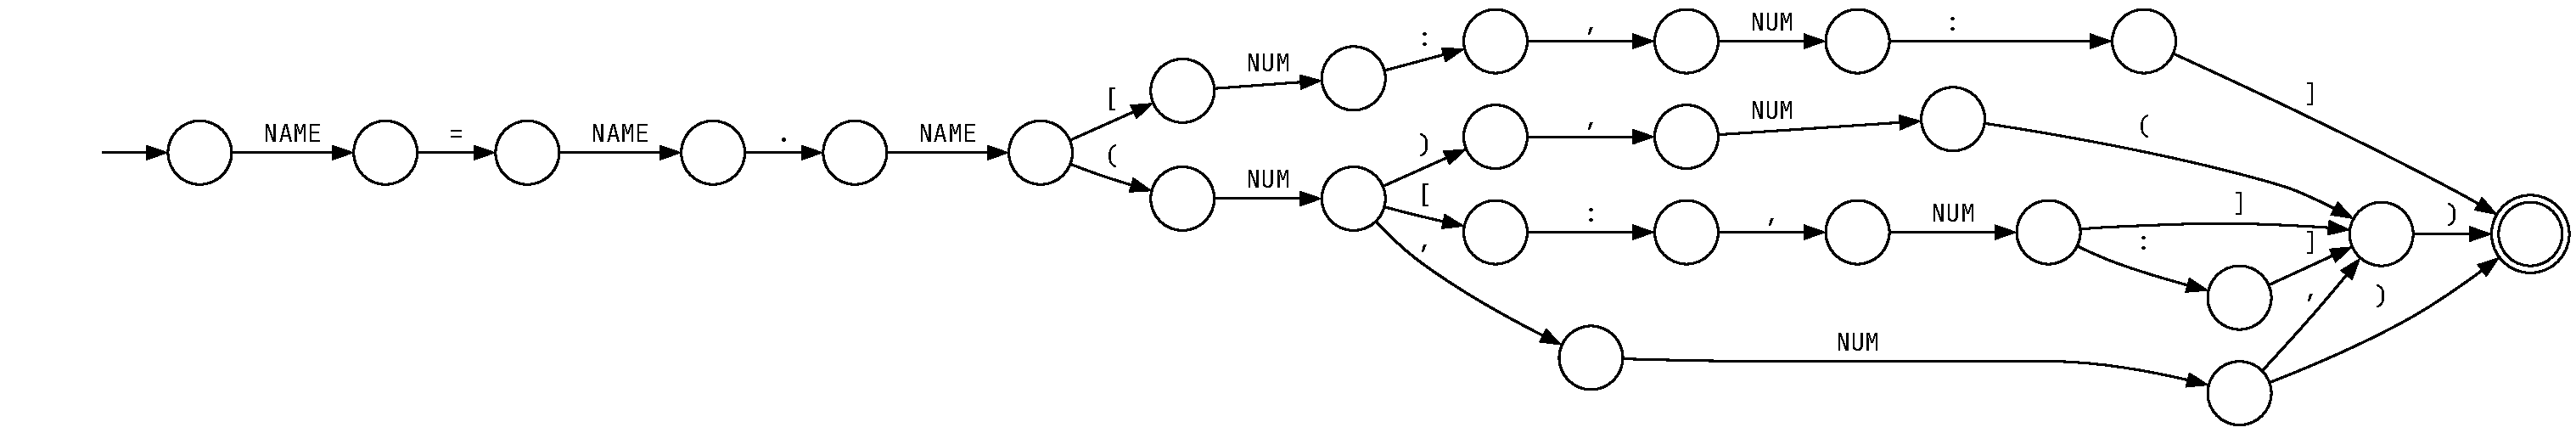
\includegraphics[width=0.9\textwidth]{../popl2025/exampleDFA.pdf}
\caption{$L(\scriptsize{\texttt{NAME = NAME . NAME ( NUM : , NUM : )}}, 2) \cap \ell_\textsc{Python}$}
\end{figure}
\end{frame}

\begin{frame}[fragile]{Decoding the DFA in order of normalized log likelihood}
\vspace{-0.3cm}
\begin{algorithm}[H]
\caption{Steerable DFA walk}
\label{alg:adaptive}
\begin{algorithmic}[1]
\Require $\mathcal{A} = \langle Q, \Sigma, \delta, I, F\rangle$ DFA, $P_\theta: \Sigma^d \rightarrow \mathbb{R}$ Markov chain

\State $\mathcal{T} \gets \varnothing \text{ total trajectories}, \mathcal{P} \gets \big[\langle \varepsilon, i, 0\rangle \mid i \in I\big] \text{ partial trajectories}$
%\State $[\mathcal{T, P}]\texttt{.comparator} = \lambda\langle\sigma, q, \gamma\rangle.(\frac{\gamma}{|\sigma|})$
\Repeat
\State \textbf{let }$\langle \sigma, q, \gamma \rangle = \texttt{head}(\mathcal{P})$ \textbf{in}
%\State $\mathcal{P} \gets \texttt{tail}(\mathcal{P})$
% For loop:
\State \phantom{\textbf{let }}$\mathbf{T} = \big\{\langle s\sigma, q', \gamma - \log P_\theta(s \mid \sigma_{1..d-1}) \rangle\mid (q\overset{s}{\rightarrow}q') \in \delta\big\}$
\For{$\langle \sigma, q, \gamma \rangle = T \in \mathbf{T}$}
\If {$\exists s: \Sigma, q': Q \mid (q\overset{s}{\rightarrow} q')\in\delta$}
\State $\mathcal{P} \gets \texttt{tail}(\mathcal{P}) \oplus T$ \Comment{Add partial trajectory to PQ.}
\EndIf
\If {$q \in F$}
\State $\mathcal{T} \gets \mathcal{T} \oplus T$ \Comment{Accepting state reached, add to queue.}
\EndIf
\EndFor
\Until{interrupted or $\mathcal{P}=\varnothing$.}
\State \Return $\big[\sigma_{|\sigma|..1} \mid \langle \sigma, q, \gamma \rangle = T \in \mathcal{T}\big]$ \Comment{Return in sorted order}
\end{algorithmic}
\end{algorithm}
\end{frame}

%\begin{frame}[fragile]{A birds eye view of the algorithm}
%  \begin{figure}[H]
%    \adjustbox{scale=0.75,center}{%
%      \[\begin{tikzcd}[row sep=large, col sep=huge]
%          \text{String} && \text{Grammar} && \err{\text{String}} \\
%          [-20pt] \highlight{\Sigma}^{n-1} \arrow[dr] & \text{\underline{Parsing}} & \mathcal{G}_\varepsilon \arrow[u, dashed, no head, color=gray] \arrow[dl]\arrow[ddl, bend left] \arrow[ddd, dashed, no head, color=gray] \arrow[dr]\arrow[ddr, bend right] & \text{\underline{Repair}} & \err{\Sigma^{n-1}} \arrow[dl] \\
%          & V^{n-1} \arrow[d] & & (V_\varepsilon \cup \{\texttt{\_}\})^{n+q} \arrow[d, shift left]\arrow[d, shift right] & \\
%          & \mathbb{Z}_2^{n\times n \times |V|} \arrow[d, shift left] \arrow[d, shift right] & & \mathbb{Z}^{(n+q)^2 \times |V_\varepsilon|}_2 \rightarrow \mathbb{Z}_2^{|V_{\varepsilon}|} \arrow[d, shift left]\arrow[d, shift right] & \\
%          & CST & \phantom{.} & \left\langle (\highlight{\Sigma} \setminus \{\varepsilon\})^*, CST \right\rangle &
%      \end{tikzcd}\]
%    }
%  \end{figure}
%  Our algorithm produces set of concrete syntax trees (CSTs) for a given valid string. Otherwise, if the string contains an error, the algorithm generates a set of admissible corrections, alongside their CSTs.
%\end{frame}

\section{Error Correction}\label{sec:error-correction}

%\begin{frame}[fragile]{Sampling without replacement}
%Let $A$ be a complicated space we do not know how to sample from.
%\begin{figure}
%\centering
%\begin{tikzpicture}[ele/.style={fill=black,circle,minimum width=.8pt,inner sep=1pt},every fit/.style={ellipse,draw,minimum width=5pt,inner sep=10pt}]
%\node[ele,label=left:$a$] (a1) at (0,3) {};
%\node[ele,label=left:$b$] (a2) at (0,2) {};
%\node[ele,label=left:$c$] (a3) at (0,1) {};
%%\node[ele,label=left:$d$] (a4) at (0,1) {};
%
%\node[ele,,label=right:$1$] (b1) at (4,4) {};
%\node[ele,,label=right:$2$] (b2) at (4,3) {};
%\node[ele,,label=right:$3$] (b3) at (4,2) {};
%\node[ele,,label=right:$4$] (b4) at (4,1) {};
%
%\node[draw,fit= (a1) (a2) (a3),minimum width=2.5cm,label=below:$A$] {} ;
%\node[draw,fit= (b1) (b2) (b3) (b4),minimum width=2.5cm,label=below:$\mathbb{N}$] {} ;
%\draw[->,shorten <=2pt,shorten >=2pt] (a1) -- (b4);
%\draw[->,shorten <=2pt,shorten >=2] (a2) -- (b2);
%\draw[->,shorten <=2pt,shorten >=2] (a3) -- (b1);
%%\draw[->,shorten <=2pt,shorten >=2] (a4) -- (b3);
%\end{tikzpicture}
%\end{figure}
%We want a permutation mapping $f: A \rightarrow \mathbb{N} \mid \forall a \in A \exists i \in \mathbb{N}.f^{-1}(i) = a$. Then we can just sample $i \sim \mathbb{N}$ without replacement and apply $f^{-1}(i)$.
%\end{frame}

%\begin{frame}[fragile]{Error Correction: Levenshtein q-Balls}
%  Now that we have a reliable method to fix \textit{localized} errors, $S: \mathcal{G} \times (\Sigma\cup\{\varepsilon, \texttt{\texttt{\_}}\})^n \rightarrow \{\Sigma^n\}\subseteq \mathcal{L}_\mathcal{G}$, given some unparseable string, i.e., $\err{\sigma_1\ldots\:\sigma_n}: \highlight{\Sigma}^n \cap\mathcal{L}_\mathcal{G}^\complement$, where should we put holes to obtain a parseable $\sigma' \in \mathcal{L}_\mathcal{G}$? One way to do so is by sampling repairs, $\bm{\sigma}\sim\Sigma^{n\pm q}\cap\Delta_{q}(\err{\sigma})$ from the Levenshtein q-ball centered on $\err{\sigma}$, i.e., the space of all admissible edits with Levenshtein distance $\leq q$ (this is loosely analogous to a finite difference approximation). To admit variable-length edits, we first add an $\varepsilon^+$-production to each unit production:\vspace{5pt}
%
%  \begin{prooftree}
%    \AxiomC{$\mathcal{G} \vdash \varepsilon \in \Sigma$}
%    \RightLabel{$\varepsilon\textsc{-dup}$}
%    \UnaryInfC{$\mathcal{G} \vdash (\varepsilon^+ \rightarrow \varepsilon \mid \varepsilon^+\:\varepsilon^+) \in P$}
%  \end{prooftree}
%
%  \begin{prooftree}
%    \AxiomC{$\mathcal{G} \vdash (A \rightarrow B) \in P$}
%    \RightLabel{$\varepsilon^+\textsc{-int}$}
%    \UnaryInfC{$\mathcal{G} \vdash (A \rightarrow B\:\varepsilon^+ \mid \varepsilon^+\:B \mid B) \in P$}
%  \end{prooftree}
%\end{frame}
%
%\begin{frame}[fragile]{Error Correction: d-Subset Sampling}
%  \noindent Next, suppose $U: \mathbb{Z}_2^{m\times m}$ is a matrix whose structure is shown in Eq.~\ref{eq:lfsr}, wherein $C$ is a primitive polynomial over $\mathbb{Z}_2^m$ with coefficients $C_{1\ldots m}$ and semiring operators $\oplus := \veebar, \otimes := \land$:\vspace{-5pt}
%
%  \begin{align}
%    U^tV = \begin{pNiceMatrix}[nullify-dots,xdots/line-style=loosely dotted]
%             C_1    & \cdd  &       &       & C_m \\
%             \top   & \circ & \cdd  &       & \circ \\
%             \circ  & \ddd  & \ddd  &       & \vdd \\
%             \vdd   & \ddd  &       &       & \\
%             \circ  & \cdd  & \circ & \top  & \circ
%    \end{pNiceMatrix}^t
%    \begin{pNiceMatrix}[nullify-dots,xdots/line-style=loosely dotted]
%      V_1 \\
%      \vdd\\
%      \\
%      \\
%      V_m
%    \end{pNiceMatrix}\label{eq:lfsr}
%  \end{align}
%
%  \noindent Since $C$ is primitive, the sequence $\mathbf{S} = (U^{0 \ldots 2^m-1}V)$ must have \textit{full periodicity}, i.e., for all $i, j \in[0, 2^m)$, ${\mathbf{S}_i = \mathbf{S}_j \Rightarrow i = j}$. To uniformly sample $\bm\sigma$ without replacement, we first form an injection $\mathbb{Z}_2^m\rightharpoonup\stirlingii{n}{d}\times\Sigma_\varepsilon^{2d}$ using a combinatorial number system, cycle over $\mathbf{S}$, then discard samples which have no witness in $\stirlingii{n}{d}\times\Sigma_\varepsilon^{2d}$. This method requires $\widetilde{\mathcal O}(1)$ per sample and $\widetilde{\mathcal O}\left({n \choose d}|\Sigma + 1|^{2d}\right)$ to exhaustively search $\stirlingii{n}{d}\times\Sigma_\varepsilon^{2d}$.
%\end{frame}
%
%\begin{frame}[fragile]{Error Correction: Sketch Templates}
%  Finally, to sample $\bm{\sigma}\sim\Delta_{q}(\err{\sigma})$, we enumerate a series of sketch templates $H(\sigma, i) = \sigma_{1\ldots i-1}\:\text{\texttt{\_} \texttt{\_}}\:\sigma_{i+1\ldots n}$ for each $i \in \cdot \in \stirlingii{n}{d}$ and $d \in 1\ldots q$, then solve for $\mathcal{M}_{\bm\sigma}^*$. If $S \in \Lambda^*_{\bm\sigma}?$ has a solution, each edit in each $\sigma' \in \bm\sigma$ will match exactly one of the following seven edit patterns:\vspace{-10pt}
%
%  \begin{align*}
%    \text{Deletion}&=\begin{cases}
%                       \,\ldots\sigma_{i-1}\:\text{\hlred{$\gamma_1$}\:\hlred{$\gamma_2$}}\:\sigma_{i+1}\ldots\hspace{0.2cm}\gamma_{1, 2} = \varepsilon\label{eq:del}
%    \end{cases}\\
%    \text{Substitution}&=\begin{cases}
%         \ldots\sigma_{i-1}\:\text{\hlorange{$\gamma_1$}\:\hlred{$\gamma_2$}}\:\sigma_{i+1}\ldots\hspace{0.2cm}\gamma_1 \neq \varepsilon \land \gamma_2 = \varepsilon\\
%         \ldots\sigma_{i-1}\:\text{\hlred{$\gamma_1$}\:\hlorange{$\gamma_2$}}\:\sigma_{i+1}\ldots\hspace{0.2cm}\gamma_1 = \varepsilon \land \gamma_2 \neq \varepsilon\\
%         \ldots\sigma_{i-1}\:\text{\hlorange{$\gamma_1$}\:\hlorange{$\gamma_2$}}\:\sigma_{i+1}\ldots\hspace{0.2cm}\{\gamma_1, \gamma_2\}\cap\{\varepsilon, \sigma_i\} = \varnothing
%    \end{cases}\\
%    \text{Insertion}&=\begin{cases}
%        \ldots\sigma_{i-1}\:\text{\hlgreen{$\gamma_1$}\:\hlorange{$\gamma_2$}}\:\sigma_{i+1}\ldots\hspace{0.2cm}\gamma_1 = \sigma_i \land \gamma_2 \notin \{\varepsilon,  \sigma_i\}\label{eq:ins2}\\
%        \ldots\sigma_{i-1}\:\text{\hlorange{$\gamma_1$}\:\hlgreen{$\gamma_2$}}\:\sigma_{i+1}\ldots\hspace{0.2cm}\gamma_1 \notin \{\varepsilon, \sigma_i\} \land \gamma_2 = \sigma_i\label{eq:ins1}\\
%        \ldots\sigma_{i-1}\:\text{\hlgreen{$\gamma_1$}\:\hlgreen{$\gamma_2$}}\:\sigma_{i+1}\ldots\hspace{0.2cm}\gamma_{1,2} = \sigma_i\label{eq:copy}
%    \end{cases}
%  \end{align*}
%\end{frame}



%\begin{frame}[fragile]{Level I: Known Error Locations}
%  \begin{figure}[H]
%    \hspace{-0.25cm}
%    \begin{tikzpicture}
%      \begin{axis}[
%        width=8.3cm,
%        height=6cm,
%        title={\hspace{-1cm}\textbf{Latency with known locations}},
%        ybar,
%        bar width=6pt,
%        xlabel={Number of holes},
%        ylabel={ms to synthesize 10 repairs},
%        xtick=data,
%        axis x line*=bottom,
%        axis y line*=left,
%        ytick pos=left,
%        xticklabels from table={\loctimings}{holes},
%        ymajorgrids,
%        legend pos=north west,
%        legend columns=2,
%        error bars/y dir=both,
%        error bars/y explicit
%      ]
%        \addplot table [x expr=\coordindex, y=d1, y error=d1err]{\loctimings};
%        \addplot table [x expr=\coordindex, y=d2, y error=d2err]{\loctimings};
%        \addplot table [x expr=\coordindex, y=d3, y error=d3err]{\loctimings};
%        \addplot table [x expr=\coordindex, y=d4, y error=d4err]{\loctimings};
%        \legend{Dyck-1, Dyck-2, Dyck-3, Dyck-4}
%      \end{axis}
%    \end{tikzpicture}
%  \end{figure}
%\end{frame}
%
%\begin{frame}[fragile]{Level II: Unknown Locations, Fixed Error Count}
%  \begin{figure}[H]
%    \hspace{-0.25cm}
%    \begin{tikzpicture}
%      \begin{axis}[
%        width=8.3cm,
%        height=6cm,
%        title={\hspace{-1cm}\textbf{Latency with unknown locations}},
%        ybar,
%        bar width=20pt,
%        xlabel={Number of errors},
%        ylabel={ms to synthesize 1 repair},
%        xtick=data,
%        axis x line*=bottom,
%        axis y line*=left,
%        enlarge x limits={abs=0.5},
%        ymode=log,
%        ytick pos=left,
%        xticklabels from table={\unloctimings}{errors},
%        ymajorgrids,
%        legend pos=north west,
%        error bars/y dir=both,
%        error bars/y explicit
%      ]
%        \addplot table [x expr=\coordindex, y=d1]{\unloctimings};
%        \addplot table [x expr=\coordindex, y=d2]{\unloctimings};
%        \addplot table [x expr=\coordindex, y=d3]{\unloctimings};
%        \legend{Dyck-1, Dyck-2, Dyck-3}
%      \end{axis}
%    \end{tikzpicture}
%  \end{figure}
%\end{frame}
%
%\begin{frame}[fragile]{Level III: MiniGithub, Unknown Count, Synthetic Errors}
%  \begin{figure}[H]
%    \centering{\textbf{Synthetic error correction accuracy}}\\
%    \vspace{0.25cm}
%%\adjustbox{scale=0.48,center}{%
%    \begin{tikzpicture}
%      \begin{axis}
%        [
%        width=8.3cm,
%        height=6.6cm,
%%    title={\hspace{-1cm}\textbf{Java Brackets}},
%        ybar,
%        bar width=10pt,
%        xlabel={$|\Sigma^*|$},
%        ylabel={Parser acceptance},
%        xtick=data,
%        axis x line*=bottom,
%        axis y line*=left,
%        enlarge x limits={abs=0.5},
%        ytick pos=left,
%        xticklabels from table={\syntheticerrors}{len},
%        ymajorgrids,
%        legend pos=north east,
%        legend columns=3,
%        error bars/y dir=both,
%        error bars/y explicit
%        ]
%        \addplot table [x expr=\coordindex, y=10s]{\syntheticerrors};
%        \addplot table [x expr=\coordindex, y=30s]{\syntheticerrors};
%        \addplot table [x expr=\coordindex, y=60s]{\syntheticerrors};
%        \legend{10s, 30s, 60s}
%      \end{axis}
%    \end{tikzpicture}
%  \end{figure}
%\end{frame}
%
%\begin{frame}[fragile]{Level IV: BIFI Dataset, Unknown Count, Real Errors}
%  \begin{figure}[H]
%    \hspace{-0.25cm}
%    \begin{tikzpicture}
%      \begin{axis}
%        [
%        width=8.3cm,
%        height=6.6cm,
%        title={\hspace{-1cm}\textbf{Organic error correction accuracy}},
%        ybar,
%        bar width=10pt,
%        xlabel={$|\Sigma^*|$},
%        ylabel={Parser acceptance},
%        xtick=data,
%        axis x line*=bottom,
%        axis y line*=left,
%        enlarge x limits={abs=0.5},
%        ytick pos=left,
%        xticklabels from table={\naturalerrors}{len},
%        ymajorgrids,
%        y tick label style={/pgf/number format/.cd,%
%        scaled y ticks = false,
%        set thousands separator={},
%        fixed},
%        legend pos=north east,
%        legend columns=3,
%        error bars/y dir=both,
%        error bars/y explicit
%        ]
%        \addplot table [x expr=\coordindex, y=10s]{\naturalerrors};
%        \addplot table [x expr=\coordindex, y=30s]{\naturalerrors};
%        \addplot table [x expr=\coordindex, y=60s]{\naturalerrors};
%        \legend{10s, 30s, 60s}
%      \end{axis}
%    \end{tikzpicture}
%  \end{figure}
%\end{frame}

\begin{frame}[fragile]{Characteristics of the repair dataset}
\begin{figure}[h!]
\begin{tikzpicture}[scale=0.52]
\begin{axis}[
ybar,
bar width=5pt,
xlabel={Length $(|\err\sigma|)$},
ylabel={Frequency},
title={Cumulative length distribution},
axis x line*=bottom,
axis y line*=left,
ymin=0,
ymax=65,
xtick=data,
xticklabels={,,<30,,,<60,,,<90,},
ymajorgrids=true,
grid style=dashed,
width=0.45\textwidth,
height=0.3\textwidth
]

\addplot[fill=black!30] table {
X Y
1 7.60
2 14.52
3 22.01
4 30.54
5 37.82
6 44.30
7 49.68
8 55.21
9 59.75
10 63.59
};
\draw[red, dashed] (axis cs:8.5,0) -- (axis cs:8.5,65);
\end{axis}
\end{tikzpicture}
\begin{tikzpicture}[scale=0.52]
\begin{axis}[
ybar,
bar width=5pt,
title={Human repair distance},
xlabel={Edits, $\Delta(\err\sigma, \sigma')$},
ylabel={Frequency},
axis x line*=bottom,
axis y line*=left,
xtick=data,
ymajorgrids=true,
grid style=dashed,
xticklabels={,\leq 2,,\leq 4,,\leq 6,,\leq 8,,\leq 10},
ytick={0, 20, 40, 60, 80, 100},
ymin=0,
width=0.45\textwidth,
height=0.3\textwidth
]
\addplot[fill=black!30] table {
X Y
1  31.48
2  47.52
3  54.89
4  60.44
5  63.88
6  66.38
7  68.02
8  70.04
9  71.49
10 72.22
};
\draw[red, dashed] (axis cs:4.5,0) -- (axis cs:4.5,80);
\end{axis}
\end{tikzpicture}
\begin{tikzpicture}[scale=0.52]
\begin{axis}[
ybar,
bar width=5pt,
xlabel={Beginning $\longleftrightarrow$ End},
ylabel={Frequency},
title={Normalized edit locations},
axis x line*=bottom,
axis y line*=left,
ymin=0,
ymax=35,
xtick=data,
xticklabels={0\%,,,,,,,,,100\%},
ymajorgrids=true,
grid style=dashed,
width=0.45\textwidth,
height=0.3\textwidth
]

\addplot[fill=black!30] table {
X Y
10 11.6539
20 5.7252
30 6.2087
40 5.9542
50 5.5980
60 7.9389
70 7.0738
80 6.9466
90 12.4173
100 30.4835
};
\end{axis}
\end{tikzpicture}
%    \begin{tikzpicture}
%      \begin{axis}[
%        ybar,
%        bar width=5pt,
%        title={Intra-patch edit distance},
%        xlabel={Caret distance},
%        ylabel={Frequency},
%        axis x line*=bottom,
%        axis y line*=left,
%        xtick=data,
%        ymajorgrids=true,
%        grid style=dashed,
%        xticklabels={1,2,3,4,5,6,7,8,9,10+},
%        width=0.45\textwidth,
%        height=0.3\textwidth
%      ]
%
%        \addplot table {
%          X Y
%          1 40.66
%          2 15.00
%          3 5.80
%          4 4.86
%          5 4.26
%          6 2.98
%          7 2.05
%          8 2.73
%          9 1.62
%          10 13.64
%        };
%      \end{axis}
%    \end{tikzpicture}
\begin{tikzpicture}[scale=0.52]
\begin{axis}[
legend cell align={left},
legend style={fill opacity=1, draw opacity=1, text opacity=1, draw=lightgray204, legend columns=-1, legend pos=north east, legend style={at={(0.5,1.8)},anchor=north}},
xlabel={$|\err\sigma|$},
ylabel={Stable region},
title={Stability profile},
ybar,
axis lines*=left,
xtick={0, 10, 20, 30, 40, 50, 60, 70},
ytick={0, 0.2, 0.4, 0.6, 0.8, 1.0},
xticklabels={, {[}10{,}20{)}, , {[}30{,}40{)}, , {[}50{,}60{)}, , {[}70{,}80{)}},
yticklabels={0, 0.2, 0.4, 0.6, 0.8, 1.0},
x tick label style={font=\scriptsize},
ymax=1.0,
ymin=0.0,
bar width=3pt,
grid style=dashed,
ymajorgrids=true,
width=0.45\textwidth,
height=0.3\textwidth
]
\addlegendimage{empty legend}
\addlegendentry{$\Delta(\err\sigma, \sigma')=$}
\addlegendimage{ybar,ybar legend,draw=none,green,fill=green!50}
\addlegendentry{1,}
\addlegendimage{ybar,ybar legend,draw=none,blue,fill=blue!50}
\addlegendentry{2,}
\addlegendimage{ybar,ybar legend,draw=none,orange,fill=orange!50}
\addlegendentry{3}
\addplot[green, fill=green!50] coordinates {(0, 0.80) (10, 0.91) (20, 0.96) (30, 0.97) (40, 0.99) (50, 0.99) (60, 0.99) (70, 0.99)};
\addplot[blue, fill=blue!50] coordinates {(0, 0.35) (10, 0.59) (20, 0.69) (30, 0.73) (40, 0.79) (50, 0.82) (60, 0.84) (70, 0.86)};
\addplot[orange, fill=orange!50] coordinates {(0, 0.23) (10, 0.45) (20, 0.58) (30, 0.66) (40, 0.70) (50, 0.77) (60, 0.78) (70, 0.86)};
\end{axis}
\end{tikzpicture}
\caption{Repair statistics across the StackOverflow dataset, of which Tidyparse can handle about half in under $\sim$30s and $\sim$150 GB. Larger repairs and edit distances are possible, albeit requiring additional time and memory. The stability profile measures the average fraction of all edit locations that were never altered by any repair in the $L\big(\err\sigma, \Delta(\err\sigma, \sigma')\big)$-ball across repairs of varying length and distance.}\label{fig:patch_stats}
\end{figure}
\end{frame}

\begin{frame}[fragile]{Ranked repair}
We train on lexical n-grams using the standard MLE for Markov chains. To score the repairs, we use the conventional length-normalized NLL:

\begin{equation}
\text{NLL}(\sigma) = -\frac{1}{|\sigma|}\sum_{i=1}^{|\sigma|}\log P_\theta(\sigma_i \mid \sigma_{i-1}\ldots\sigma_{i-n})
\end{equation}

For each retrieved set $\hat{A} \subseteq A$ drawn before a predetermined timeout and each $\sigma \in \hat{A}$, we score the repair and return $\hat{A}$ in ascending order.

To evaluate the quality of our ranking, we use the Precision@k statistic. Specifically, given a repair model, $R: \Sigma^* \rightarrow 2^{\Sigma^*}$ and a parallel corpus, $\mathcal{D}_{\text{test}}$, of errors ($\sigma^\dagger$) and repairs ($\sigma'$), we define Precision@k as:

\begin{equation}
\text{Precision@k}(R) = \frac{1}{|\mathcal{D}_{\text{test}}|}\sum_{\langle\sigma^\dagger, \sigma'\rangle \in \mathcal{D}_{\text{test}}} \mathds{1}\big[\sigma' \in \argmax_{\bm{\sigma} \subset R(\sigma^\dagger), |\bm{\sigma}| \leq k}\sum_{\sigma \in \bm{\sigma}}\text{NLL}(\sigma)\big]
\end{equation}
\end{frame}

\begin{frame}[fragile]{Precision and latency comparison}
\begin{figure}[h!]
\resizebox{.24\textwidth}{!}{\begin{tikzpicture}
  \begin{axis}[
    xlabel={Snippet length, $|\sigma|$},
    ylabel={Precision@1},
    title={\Large\textbf{Tidyparse Repair Precision@1}},
    ybar,
    axis lines*=left,
    xtick={0, 10, 20, 30, 40, 50, 60, 70},
    ytick={0, 0.1, 0.2, 0.3, 0.4, 0.5, 0.6, 0.7, 0.8, 0.9, 1.0},
    xticklabels={{(}0{,}10{)}, {[}10{,}20{)}, {[}20{,}30{)}, {[}30{,}40{)}, {[}40{,}50{)}, {[}50{,}60{)}, {[}60{,}70{)}, {[}70{,}80{)}},
    x tick label style={font=\scriptsize},
    ymax=0.7,
    ymin=0.0,
    bar width=4pt,
  ]
%  \addplot[green, fill=green!50] coordinates { (0, 0.5) (10, 0.1827956989247312) (20, 0.08366533864541832) (30, 0.06572769953051644) (40, 0.016) (50, 0.020833333333333332) (60, 0.0) (70, 0.014705882352941176) };
%  \addplot[blue, fill=blue!50] coordinates { (0, 0.39285714285714285) (10, 0.42105263157894735) (20, 0.2037037037037037) (30, 0.20588235294117646) (40, 0.14666666666666667) (50, 0.06349206349206349) (60, 0.08) (70, 0.08571428571428572) };
%  \addplot[orange, fill=orange!50] coordinates { (0, 0.0) (10, 0.0) (20, 0.03125) (30, 0.10526315789473684) (40, 0.0) (50, 0.08333333333333333) (60, 0.06666666666666667) (70, 0.0) };
%  \addplot[green, fill=green!50] coordinates { (0, 1.0) (10, 1.0) (20, 1.0) (30, 1.0) (40, 1.0) (50, 1.0) (60, 1.0) (70, 1.0) };
%  \addplot[blue, fill=blue!50] coordinates { (0, 1.0) (10, 1.0) (20, 1.0) (30, 1.0) (40, 1.0) (50, 1.0) (60, 1.0) (70, 1.0) };
%  \addplot[orange, fill=orange!50] coordinates { (0, 0.25) (10, 0.14285714285714285) (20, 0.3125) (30, 0.42105263157894735) (40, 0.375) (50, 0.25) (60, 0.6) (70, 0.3333333333333333) };
%  \addplot[green, fill=green!50] coordinates { (0, 0.53125) (10, 0.22043010752688172) (20, 0.14741035856573706) (30, 0.0892018779342723) (40, 0.048) (50, 0.03125) (60, 0.0) (70, 0.029411764705882353) };
%  \addplot[blue, fill=blue!50] coordinates { (0, 0.39285714285714285) (10, 0.3684210526315789) (20, 0.17592592592592593) (30, 0.18627450980392157) (40, 0.14666666666666667) (50, 0.09523809523809523) (60, 0.04) (70, 0.11428571428571428) };
%  \addplot[orange, fill=orange!50] coordinates { (0, 0.0) (10, 0.0) (20, 0.03125) (30, 0.10526315789473684) (40, 0.0) (50, 0.16666666666666666) (60, 0.06666666666666667) (70, 0.0) };
%  \addplot[green, fill=green!50] coordinates { (0, 0.5) (10, 0.25) (20, 0.4166666666666667) (30, 0.47368421052631576) (40, 0.5) (50, 0.29411764705882354) (60, 0.5) (70, 0.3333333333333333) };
%  \addplot[blue, fill=blue!50] coordinates { (0, 0.8571428571428571) (10, 0.6363636363636364) (20, 0.7142857142857143) (30, 0.5833333333333334) (40, 0.45454545454545453) (50, 0.5714285714285714) (60, 0.14285714285714285) (70, 0.36363636363636365) };
%  \addplot[orange, fill=orange!50] coordinates { (0, 0.6) (10, 0.23076923076923078) (20, 0.3125) (30, 0.3) (40, 0.18181818181818182) (50, 0.3125) (60, 0.7) (70, 0.16666666666666666) };
  \addplot[green, fill=green!50] coordinates { (0, 0.36363636363636365) (10, 0.5416666666666666) (20, 0.4482758620689655) (30, 0.4067796610169492) (40, 0.3956043956043956) (50, 0.3333333333333333) (60, 0.47368421052631576) (70, 0.2608695652173913) };
  \addplot[blue, fill=blue!50] coordinates { (0, 0.6363636363636364) (10, 0.6610169491525424) (20, 0.5125) (30, 0.5) (40, 0.35714285714285715) (50, 0.4375) (60, 0.2972972972972973) (70, 0.3488372093023256) };
  \addplot[orange, fill=orange!50] coordinates { (0, 0.2222222222222222) (10, 0.15384615384615385) (20, 0.12582781456953643) (30, 0.13380281690140844) (40, 0.12037037037037036) (50, 0.1792452830188679) (60, 0.17391304347826086) (70, 0.11594202898550725) };
  \end{axis}
\end{tikzpicture}

%                                    TIDY-GWA                     TIDY-CFG                  TIDY-ENUM
%(|σ|∈[0, 10), Δ=1): Top-1/total:    56 / 100 = 0.56               54 / 99 = 0.55            57 / 100 = 0.57
%(|σ|∈[0, 10), Δ=2): Top-1/total:    37 / 100 = 0.37              19 / 100 = 0.19            22 / 100 = 0.22
%(|σ|∈[0, 10), Δ=3): Top-1/total:      9 / 50 = 0.18                6 / 50 = 0.12              6 / 50 = 0.12

%(|σ|∈[10, 20), Δ=1): Top-1/total:   44 / 100 = 0.44              42 / 100 = 0.42            45 / 100 = 0.45
%(|σ|∈[10, 20), Δ=2): Top-1/total:   28 / 100 = 0.28              13 / 100 = 0.13            14 / 100 = 0.14
%(|σ|∈[10, 20), Δ=3): Top-1/total:   20 / 100 = 0.20               9 / 100 = 0.09             8 / 100 = 0.08

%(|σ|∈[20, 30), Δ=1): Top-1/total:   43 / 100 = 0.43              49 / 100 = 0.49            49 / 100 = 0.49
%(|σ|∈[20, 30), Δ=2): Top-1/total:   26 / 100 = 0.26              13 / 100 = 0.13            18 / 100 = 0.18
%(|σ|∈[20, 30), Δ=3): Top-1/total:    19 / 99 = 0.19                8 / 99 = 0.08              8 / 99 = 0.08

%(|σ|∈[30, 40), Δ=1): Top-1/total:   49 / 100 = 0.49              43 / 100 = 0.43            48 / 100 = 0.48
%(|σ|∈[30, 40), Δ=2): Top-1/total:   24 / 100 = 0.24              15 / 100 = 0.15            18 / 100 = 0.18
%(|σ|∈[30, 40), Δ=3): Top-1/total:   15 / 100 = 0.15              10 / 100 = 0.10             6 / 100 = 0.06

%(|σ|∈[40, 50), Δ=1): Top-1/total:   55 / 100 = 0.55              56 / 100 = 0.56            57 / 100 = 0.57
%(|σ|∈[40, 50), Δ=2): Top-1/total:   19 / 100 = 0.19              21 / 100 = 0.21            18 / 100 = 0.18
%(|σ|∈[40, 50), Δ=3): Top-1/total:   10 / 100 = 0.10               8 / 100 = 0.08             5 / 100 = 0.05

%(|σ|∈[50, 60), Δ=1): Top-1/total:   55 / 100 = 0.55              67 / 100 = 0.67            53 / 100 = 0.53
%(|σ|∈[50, 60), Δ=2): Top-1/total:   25 / 100 = 0.25              16 / 100 = 0.16            21 / 100 = 0.21
%(|σ|∈[50, 60), Δ=3): Top-1/total:    9 / 100 = 0.09               9 / 100 = 0.09             7 / 100 = 0.07

%(|σ|∈[60, 70), Δ=1): Top-1/total:   53 / 100 = 0.53              56 / 100 = 0.56            60 / 100 = 0.60
%(|σ|∈[60, 70), Δ=2): Top-1/total:   23 / 100 = 0.23              15 / 100 = 0.15            10 / 100 = 0.10
%(|σ|∈[60, 70), Δ=3): Top-1/total:   11 / 100 = 0.11               5 / 100 = 0.05             2 / 100 = 0.02

%(|σ|∈[70, 80), Δ=1): Top-1/total:   57 / 100 = 0.57              62 / 100 = 0.62            63 / 100 = 0.63
%(|σ|∈[70, 80), Δ=2): Top-1/total:   18 / 100 = 0.18              12 / 100 = 0.12            15 / 100 = 0.15
%(|σ|∈[70, 80), Δ=3): Top-1/total:     9 / 81 = 0.11                4 / 81 = 0.05              3 / 81 = 0.04}
\resizebox{.24\textwidth}{!}{\begin{tikzpicture}
  \begin{axis}[
  xlabel={Snippet length, $|\sigma|$},
  ylabel={Precision@20k},
  title={\Large\textbf{BIFI Repair Precision@20,000}},
  legend cell align={left},
  legend style={fill opacity=0.8, draw opacity=1, text opacity=1, draw=lightgray204, legend columns=-1, legend pos=north east},
  ybar,
  axis lines*=left,
  xtick={0, 10, 20, 30, 40, 50, 60, 70},
  ytick={0, 0.1, 0.2, 0.3, 0.4, 0.5, 0.6, 0.7, 0.8, 0.9, 1.0},
  xticklabels={{(}0{,}10{)}, {[}10{,}20{)}, {[}20{,}30{)}, {[}30{,}40{)}, {[}40{,}50{)}, {[}50{,}60{)}, {[}60{,}70{)}, {[}70{,}80{)}},
  x tick label style={font=\scriptsize},
  ymax=1.0,
  ymin=0.0,
  bar width=4pt,
  ]

  \addlegendimage{empty legend}
  \addlegendentry{$\Delta(\err\sigma, \sigma')=$}
  \addlegendimage{ybar,ybar legend,draw=none,green,fill=green!50}
  \addlegendentry{1,}
  \addlegendimage{ybar,ybar legend,draw=none,blue,fill=blue!50}
  \addlegendentry{2,}
  \addlegendimage{ybar,ybar legend,draw=none,orange,fill=orange!50}
  \addlegendentry{3}

  \addplot[green, fill=green!50] coordinates   {(0, 0.65) (10, 0.67) (20, 0.71) (30, 0.63) (40, 0.60) (50, 0.62) (60, 0.59) (70, 0.64)};
  \addplot[blue, fill=blue!50] coordinates     {(0, 0.52) (10, 0.41) (20, 0.35) (30, 0.31) (40, 0.27) (50, 0.27) (60, 0.21) (70, 0.22)};
  \addplot[orange, fill=orange!50] coordinates {(0, 0.25) (10, 0.08) (20, 0.08) (30, 0.17) (40, 0.11) (50, 0.17) (60, 0.08) (70, 0.08)};

  \end{axis}
\end{tikzpicture}
}
\resizebox{.24\textwidth}{!}{\begin{tikzpicture}
  \begin{axis}[
    xlabel={Snippet length, $|\sigma|$},
    ylabel={Precision@1},
    title={\Large\textbf{Seq2Parse Repair Precision@1}},
    ybar,
    axis lines*=left,
    xtick={0, 10, 20, 30, 40, 50, 60, 70},
    ytick={0, 0.1, 0.2, 0.3, 0.4, 0.5, 0.6, 0.7, 0.8, 0.9, 1.0},
    xticklabels={{(}0{,}10{)}, {[}10{,}20{)}, {[}20{,}30{)}, {[}30{,}40{)}, {[}40{,}50{)}, {[}50{,}60{)}, {[}60{,}70{)}, {[}70{,}80{)}},
    x tick label style={font=\scriptsize},
    ymax=0.6,
    ymin=0.0,
    bar width=4pt,
  ]

  \addplot[green, fill=green!50] coordinates {(0, 0.352631) (10, 0.413115) (20, 0.400502) (30, 0.378440) (40, 0.308869) (50, 0.287755) (60, 0.268817) (70, 0.210526)};
  \addplot[blue, fill=blue!50] coordinates {(0, 0.122529) (10, 0.126453) (20, 0.144192) (30, 0.118483) (40, 0.108007) (50, 0.106849) (60, 0.097403) (70, 0.122047)};
  \addplot[orange, fill=orange!50] coordinates {(0, 0.03125) (10, 0.070922) (20, 0.077348) (30, 0.087629) (40, 0.094675) (50, 0.02) (60, 0.066038) (70, 0.063291)};

  \end{axis}
\end{tikzpicture}}
\resizebox{.24\textwidth}{!}{\begin{tikzpicture}
  \begin{axis}[
    legend cell align={left},
    legend style={fill opacity=0.8, draw opacity=1, text opacity=1, draw=lightgray204, legend columns=-1, legend pos=north east},
    xlabel={Snippet length, $|\sigma|$},
    ylabel={Precision@1},
    title={\Large\textbf{BIFI Repair Precision@1}},
    ybar,
    axis lines*=left,
    xtick={0, 10, 20, 30, 40, 50, 60, 70},
    ytick={0, 0.1, 0.2, 0.3, 0.4, 0.5, 0.6, 0.7, 0.8, 0.9, 1.0},
    xticklabels={{(}0{,}10{)}, {[}10{,}20{)}, {[}20{,}30{)}, {[}30{,}40{)}, {[}40{,}50{)}, {[}50{,}60{)}, {[}60{,}70{)}, {[}70{,}80{)}},
    x tick label style={font=\scriptsize},
    ymax=1.0,
    ymin=0.0,
    bar width=4pt,
    ymajorgrids=true,
    grid style=dashed,
    tick align=outside,
    tick pos=left,
  ]
%    \addlegendimage{empty legend}
%    \addlegendentry{$\Delta(\err\sigma, \sigma')=$}
%    \addlegendimage{ybar,ybar legend,draw=none,green,fill=green!50}
%    \addlegendentry{1,}
%    \addlegendimage{ybar,ybar legend,draw=none,blue,fill=blue!50}
%    \addlegendentry{2,}
%    \addlegendimage{ybar,ybar legend,draw=none,orange,fill=orange!50}
%    \addlegendentry{3}

    \addplot[green, fill=green!50] coordinates {(0, 0.196013) (10, 0.326401) (20, 0.318538) (30, 0.272843) (40, 0.213894) (50, 0.206651) (60, 0.247525) (70, 0.179245)};
    \addplot[blue, fill=blue!50] coordinates {(0, 0.174603) (10, 0.176651) (20, 0.209573) (30, 0.19195) (40, 0.18851) (50, 0.176166) (60, 0.110787) (70, 0.106383)};
    \addplot[orange, fill=orange!50] coordinates {(0, 0.015873) (10, 0.021858) (20, 0.030435) (30, 0.02439) (40, 0.032922) (50, 0.045) (60, 0.027397) (70, 0.017094)};
  \end{axis}
\end{tikzpicture}}
\caption{Tidyparse, Seq2Parse and BIFI repair precision across length and edits.}
\end{figure}
\begin{figure}[h!]
%    \resizebox{.19\textwidth}{!}{% This file was created with tikzplotlib v0.10.1.
\begin{tikzpicture}

\definecolor{darkgray176}{RGB}{176,176,176}
\definecolor{darkviolet1270255}{RGB}{127,0,255}
\definecolor{deepskyblue3176236}{RGB}{3,176,236}
\definecolor{dodgerblue45123246}{RGB}{45,123,246}
\definecolor{royalblue8762253}{RGB}{87,62,253}

\begin{axis}[
tick align=outside,
tick pos=left,
axis lines=left,
title={\textbf{\Large\(\displaystyle \Delta\in[1,3]\) Repair Precision}},
legend style={fill opacity=0.8, draw opacity=1, text opacity=1, legend columns=1, legend pos=north west},
x grid style={darkgray176},
xlabel={Seconds},
xmin=-0.5925, xmax=8.5925,
xtick style={color=black},
xtick={0,1,2,3,4,5,6,7,8},
xticklabels={1,2,3,4,5,6,7,8,9},
y grid style={darkgray176},
ylabel={Precision@k},
ymin=0, ymax=0.6993,
ytick style={color=black}
]
\draw[draw=none,fill=darkviolet1270255] (axis cs:-0.175,0) rectangle (axis cs:0.175,0.149);
\addlegendimage{ybar,ybar legend,draw=none,fill=darkviolet1270255}
\addlegendentry{P@All}

\draw[draw=none,fill=darkviolet1270255] (axis cs:0.825,0) rectangle (axis cs:1.175,0.303);
\draw[draw=none,fill=darkviolet1270255] (axis cs:1.825,0) rectangle (axis cs:2.175,0.412);
\draw[draw=none,fill=darkviolet1270255] (axis cs:2.825,0) rectangle (axis cs:3.175,0.501);
\draw[draw=none,fill=darkviolet1270255] (axis cs:3.825,0) rectangle (axis cs:4.175,0.569);
\draw[draw=none,fill=darkviolet1270255] (axis cs:4.825,0) rectangle (axis cs:5.175,0.605);
\draw[draw=none,fill=darkviolet1270255] (axis cs:5.825,0) rectangle (axis cs:6.175,0.63);
\draw[draw=none,fill=darkviolet1270255] (axis cs:6.825,0) rectangle (axis cs:7.175,0.645);
\draw[draw=none,fill=darkviolet1270255] (axis cs:7.825,0) rectangle (axis cs:8.175,0.666);
\draw[draw=none,fill=royalblue8762253] (axis cs:-0.175,0) rectangle (axis cs:0.175,0.128);
\addlegendimage{ybar,ybar legend,draw=none,fill=royalblue8762253}
\addlegendentry{P@10}

\draw[draw=none,fill=royalblue8762253] (axis cs:0.825,0) rectangle (axis cs:1.175,0.239);
\draw[draw=none,fill=royalblue8762253] (axis cs:1.825,0) rectangle (axis cs:2.175,0.323);
\draw[draw=none,fill=royalblue8762253] (axis cs:2.825,0) rectangle (axis cs:3.175,0.374);
\draw[draw=none,fill=royalblue8762253] (axis cs:3.825,0) rectangle (axis cs:4.175,0.421);
\draw[draw=none,fill=royalblue8762253] (axis cs:4.825,0) rectangle (axis cs:5.175,0.446);
\draw[draw=none,fill=royalblue8762253] (axis cs:5.825,0) rectangle (axis cs:6.175,0.459);
\draw[draw=none,fill=royalblue8762253] (axis cs:6.825,0) rectangle (axis cs:7.175,0.469);
\draw[draw=none,fill=royalblue8762253] (axis cs:7.825,0) rectangle (axis cs:8.175,0.477);
\draw[draw=none,fill=dodgerblue45123246] (axis cs:-0.175,0) rectangle (axis cs:0.175,0.11);
\addlegendimage{ybar,ybar legend,draw=none,fill=dodgerblue45123246}
\addlegendentry{P@5}

\draw[draw=none,fill=dodgerblue45123246] (axis cs:0.825,0) rectangle (axis cs:1.175,0.206);
\draw[draw=none,fill=dodgerblue45123246] (axis cs:1.825,0) rectangle (axis cs:2.175,0.282);
\draw[draw=none,fill=dodgerblue45123246] (axis cs:2.825,0) rectangle (axis cs:3.175,0.325);
\draw[draw=none,fill=dodgerblue45123246] (axis cs:3.825,0) rectangle (axis cs:4.175,0.369);
\draw[draw=none,fill=dodgerblue45123246] (axis cs:4.825,0) rectangle (axis cs:5.175,0.392);
\draw[draw=none,fill=dodgerblue45123246] (axis cs:5.825,0) rectangle (axis cs:6.175,0.405);
\draw[draw=none,fill=dodgerblue45123246] (axis cs:6.825,0) rectangle (axis cs:7.175,0.414);
\draw[draw=none,fill=dodgerblue45123246] (axis cs:7.825,0) rectangle (axis cs:8.175,0.422);
\draw[draw=none,fill=deepskyblue3176236] (axis cs:-0.175,0) rectangle (axis cs:0.175,0.092);
\addlegendimage{ybar,ybar legend,draw=none,fill=deepskyblue3176236}
\addlegendentry{P@1}

\draw[draw=none,fill=deepskyblue3176236] (axis cs:0.825,0) rectangle (axis cs:1.175,0.18);
\draw[draw=none,fill=deepskyblue3176236] (axis cs:1.825,0) rectangle (axis cs:2.175,0.244);
\draw[draw=none,fill=deepskyblue3176236] (axis cs:2.825,0) rectangle (axis cs:3.175,0.285);
\draw[draw=none,fill=deepskyblue3176236] (axis cs:3.825,0) rectangle (axis cs:4.175,0.324);
\draw[draw=none,fill=deepskyblue3176236] (axis cs:4.825,0) rectangle (axis cs:5.175,0.343);
\draw[draw=none,fill=deepskyblue3176236] (axis cs:5.825,0) rectangle (axis cs:6.175,0.356);
\draw[draw=none,fill=deepskyblue3176236] (axis cs:6.825,0) rectangle (axis cs:7.175,0.365);
\draw[draw=none,fill=deepskyblue3176236] (axis cs:7.825,0) rectangle (axis cs:8.175,0.37);
\addplot [red, thick] coordinates {(-0.8925,0.29) (14.8925,0.29)};
\end{axis}

\end{tikzpicture}
}
\resizebox{.24\textwidth}{!}{% This file was created with tikzplotlib v0.10.1.
\begin{tikzpicture}
\begin{axis}[
legend cell align={left},
legend style={fill opacity=0.8, draw opacity=1, text opacity=1, draw=lightgray204, legend columns=-1, legend pos=north west},
tick align=outside,
tick pos=left,
axis lines*=left,
title={\(\displaystyle \Delta=1\) Repair Precision},
x grid style={darkgray176},
xlabel={Seconds},
xmin=-0.5925, xmax=8.5925,
xtick style={color=black},
xtick={0,1,2,3,4,5,6,7,8},
xticklabels={1,2,3,4,5,6,7,8,9},
y grid style={darkgray176},
ylabel={Precision@k},
ymin=0, ymax=1.03845,
ytick style={color=black}
]
\draw[draw=none,fill=darkviolet1270255] (axis cs:-0.175,0) rectangle (axis cs:0.175,0.619);
\addlegendimage{empty legend}
\addlegendentry{P@}
\addlegendimage{ybar,ybar legend,draw=none,fill=darkviolet1270255}
\addlegendentry{All}

\draw[draw=none,fill=darkviolet1270255] (axis cs:0.825,0) rectangle (axis cs:1.175,0.781);
\draw[draw=none,fill=darkviolet1270255] (axis cs:1.825,0) rectangle (axis cs:2.175,0.891);
\draw[draw=none,fill=darkviolet1270255] (axis cs:2.825,0) rectangle (axis cs:3.175,0.956);
\draw[draw=none,fill=darkviolet1270255] (axis cs:3.825,0) rectangle (axis cs:4.175,0.976);
\draw[draw=none,fill=darkviolet1270255] (axis cs:4.825,0) rectangle (axis cs:5.175,0.982);
\draw[draw=none,fill=darkviolet1270255] (axis cs:5.825,0) rectangle (axis cs:6.175,0.985);
\draw[draw=none,fill=darkviolet1270255] (axis cs:6.825,0) rectangle (axis cs:7.175,0.988);
\draw[draw=none,fill=darkviolet1270255] (axis cs:7.825,0) rectangle (axis cs:8.175,0.989);
\draw[draw=none,fill=royalblue8762253] (axis cs:-0.175,0) rectangle (axis cs:0.175,0.434);
\addlegendimage{ybar,ybar legend,draw=none,fill=royalblue8762253}
\addlegendentry{10}

\draw[draw=none,fill=royalblue8762253] (axis cs:0.825,0) rectangle (axis cs:1.175,0.556);
\draw[draw=none,fill=royalblue8762253] (axis cs:1.825,0) rectangle (axis cs:2.175,0.64);
\draw[draw=none,fill=royalblue8762253] (axis cs:2.825,0) rectangle (axis cs:3.175,0.69);
\draw[draw=none,fill=royalblue8762253] (axis cs:3.825,0) rectangle (axis cs:4.175,0.707);
\draw[draw=none,fill=royalblue8762253] (axis cs:4.825,0) rectangle (axis cs:5.175,0.71);
\draw[draw=none,fill=royalblue8762253] (axis cs:5.825,0) rectangle (axis cs:6.175,0.712);
\draw[draw=none,fill=royalblue8762253] (axis cs:6.825,0) rectangle (axis cs:7.175,0.714);
\draw[draw=none,fill=royalblue8762253] (axis cs:7.825,0) rectangle (axis cs:8.175,0.715);
\draw[draw=none,fill=dodgerblue45123246] (axis cs:-0.175,0) rectangle (axis cs:0.175,0.406);
\addlegendimage{ybar,ybar legend,draw=none,fill=dodgerblue45123246}
\addlegendentry{5}

\draw[draw=none,fill=dodgerblue45123246] (axis cs:0.825,0) rectangle (axis cs:1.175,0.517);
\draw[draw=none,fill=dodgerblue45123246] (axis cs:1.825,0) rectangle (axis cs:2.175,0.6);
\draw[draw=none,fill=dodgerblue45123246] (axis cs:2.825,0) rectangle (axis cs:3.175,0.648);
\draw[draw=none,fill=dodgerblue45123246] (axis cs:3.825,0) rectangle (axis cs:4.175,0.663);
\draw[draw=none,fill=dodgerblue45123246] (axis cs:4.825,0) rectangle (axis cs:5.175,0.667);
\draw[draw=none,fill=dodgerblue45123246] (axis cs:5.825,0) rectangle (axis cs:6.175,0.668);
\draw[draw=none,fill=dodgerblue45123246] (axis cs:6.825,0) rectangle (axis cs:7.175,0.67);
\draw[draw=none,fill=dodgerblue45123246] (axis cs:7.825,0) rectangle (axis cs:8.175,0.671);
\draw[draw=none,fill=deepskyblue3176236] (axis cs:-0.175,0) rectangle (axis cs:0.175,0.316);
\addlegendimage{ybar,ybar legend,draw=none,fill=deepskyblue3176236}
\addlegendentry{1}

\draw[draw=none,fill=deepskyblue3176236] (axis cs:0.825,0) rectangle (axis cs:1.175,0.4);
\draw[draw=none,fill=deepskyblue3176236] (axis cs:1.825,0) rectangle (axis cs:2.175,0.467);
\draw[draw=none,fill=deepskyblue3176236] (axis cs:2.825,0) rectangle (axis cs:3.175,0.504);
\draw[draw=none,fill=deepskyblue3176236] (axis cs:3.825,0) rectangle (axis cs:4.175,0.515);
\draw[draw=none,fill=deepskyblue3176236] (axis cs:4.825,0) rectangle (axis cs:5.175,0.518);
\draw[draw=none,fill=deepskyblue3176236] (axis cs:5.825,0) rectangle (axis cs:6.175,0.519);
\draw[draw=none,fill=deepskyblue3176236] (axis cs:6.825,0) rectangle (axis cs:7.175,0.52);
\draw[draw=none,fill=deepskyblue3176236] (axis cs:7.825,0) rectangle (axis cs:8.175,0.52);
\addplot [red, thick] coordinates {(-0.8925,0.39) (14.8925,0.39)};
\addplot [orange, thick] coordinates {(-0.8925,0.24) (14.8925,0.24)};
\end{axis}

\end{tikzpicture}
}
\resizebox{.24\textwidth}{!}{% This file was created with tikzplotlib v0.10.1.
\begin{tikzpicture}
\begin{axis}[
tick align=outside,
tick pos=left,
axis lines=left,
title={\(\displaystyle \Delta=2\) Repair Precision},
x grid style={darkgray176},
xlabel={Seconds},
xmin=-0.5925, xmax=8.5925,
xtick style={color=black},
xtick={0,1,2,3,4,5,6,7,8},
xticklabels={1,2,3,4,5,6,7,8,9},
y grid style={darkgray176},
ylabel={Precision@k},
ymin=0, ymax=0.9471,
ytick style={color=black}
]
\draw[draw=none,fill=darkviolet1270255] (axis cs:0.825,0) rectangle (axis cs:1.175,0.48);
\draw[draw=none,fill=darkviolet1270255] (axis cs:1.825,0) rectangle (axis cs:2.175,0.597);
\draw[draw=none,fill=darkviolet1270255] (axis cs:2.825,0) rectangle (axis cs:3.175,0.68);
\draw[draw=none,fill=darkviolet1270255] (axis cs:3.825,0) rectangle (axis cs:4.175,0.748);
\draw[draw=none,fill=darkviolet1270255] (axis cs:4.825,0) rectangle (axis cs:5.175,0.802);
\draw[draw=none,fill=darkviolet1270255] (axis cs:5.825,0) rectangle (axis cs:6.175,0.842);
\draw[draw=none,fill=darkviolet1270255] (axis cs:6.825,0) rectangle (axis cs:7.175,0.874);
\draw[draw=none,fill=darkviolet1270255] (axis cs:7.825,0) rectangle (axis cs:8.175,0.902);
\draw[draw=none,fill=royalblue8762253] (axis cs:-0.175,0) rectangle (axis cs:0.175,0.147);

\draw[draw=none,fill=royalblue8762253] (axis cs:0.825,0) rectangle (axis cs:1.175,0.197);
\draw[draw=none,fill=royalblue8762253] (axis cs:1.825,0) rectangle (axis cs:2.175,0.221);
\draw[draw=none,fill=royalblue8762253] (axis cs:2.825,0) rectangle (axis cs:3.175,0.243);
\draw[draw=none,fill=royalblue8762253] (axis cs:3.825,0) rectangle (axis cs:4.175,0.261);
\draw[draw=none,fill=royalblue8762253] (axis cs:4.825,0) rectangle (axis cs:5.175,0.274);
\draw[draw=none,fill=royalblue8762253] (axis cs:5.825,0) rectangle (axis cs:6.175,0.281);
\draw[draw=none,fill=royalblue8762253] (axis cs:6.825,0) rectangle (axis cs:7.175,0.29);
\draw[draw=none,fill=royalblue8762253] (axis cs:7.825,0) rectangle (axis cs:8.175,0.295);
\draw[draw=none,fill=dodgerblue45123246] (axis cs:-0.175,0) rectangle (axis cs:0.175,0.142);

\draw[draw=none,fill=dodgerblue45123246] (axis cs:0.825,0) rectangle (axis cs:1.175,0.19);
\draw[draw=none,fill=dodgerblue45123246] (axis cs:1.825,0) rectangle (axis cs:2.175,0.214);
\draw[draw=none,fill=dodgerblue45123246] (axis cs:2.825,0) rectangle (axis cs:3.175,0.234);
\draw[draw=none,fill=dodgerblue45123246] (axis cs:3.825,0) rectangle (axis cs:4.175,0.251);
\draw[draw=none,fill=dodgerblue45123246] (axis cs:4.825,0) rectangle (axis cs:5.175,0.263);
\draw[draw=none,fill=dodgerblue45123246] (axis cs:5.825,0) rectangle (axis cs:6.175,0.27);
\draw[draw=none,fill=dodgerblue45123246] (axis cs:6.825,0) rectangle (axis cs:7.175,0.278);
\draw[draw=none,fill=dodgerblue45123246] (axis cs:7.825,0) rectangle (axis cs:8.175,0.283);
\draw[draw=none,fill=deepskyblue3176236] (axis cs:-0.175,0) rectangle (axis cs:0.175,0.123);

\draw[draw=none,fill=deepskyblue3176236] (axis cs:0.825,0) rectangle (axis cs:1.175,0.16);
\draw[draw=none,fill=deepskyblue3176236] (axis cs:1.825,0) rectangle (axis cs:2.175,0.18);
\draw[draw=none,fill=deepskyblue3176236] (axis cs:2.825,0) rectangle (axis cs:3.175,0.196);
\draw[draw=none,fill=deepskyblue3176236] (axis cs:3.825,0) rectangle (axis cs:4.175,0.209);
\draw[draw=none,fill=deepskyblue3176236] (axis cs:4.825,0) rectangle (axis cs:5.175,0.219);
\draw[draw=none,fill=deepskyblue3176236] (axis cs:5.825,0) rectangle (axis cs:6.175,0.222);
\draw[draw=none,fill=deepskyblue3176236] (axis cs:6.825,0) rectangle (axis cs:7.175,0.227);
\draw[draw=none,fill=deepskyblue3176236] (axis cs:7.825,0) rectangle (axis cs:8.175,0.232);
\addplot [red, thick] coordinates {(-0.8925,0.15) (14.8925,0.15)};
\addplot [orange, thick] coordinates {(-0.8925,0.10) (14.8925,0.10)};
\end{axis}

\end{tikzpicture}
}
\resizebox{.24\textwidth}{!}{% This file was created with tikzplotlib v0.10.1.
\begin{tikzpicture}
\begin{axis}[
tick align=outside,
tick pos=left,
axis lines=left,
title={\textbf{\Large Repair Precision \(\mathbf{(\bm\Delta=3)}\)}},
legend style={fill opacity=0.8, draw opacity=1, text opacity=1, legend columns=1, legend pos=north west},
x grid style={darkgray176},
xlabel={Seconds},
xmin=-0.5925, xmax=8.5925,
xtick style={color=black},
xtick={0,1,2,3,4,5,6,7,8},
xticklabels={10,20,30,40,50,60,70,80,90},
y grid style={darkgray176},
ylabel={Precision@k},
ymin=0, ymax=0.74655,
ytick style={color=black}
legend style={draw=none}
]
\draw[draw=none,fill=darkviolet1270255] (axis cs:0.825,0) rectangle (axis cs:1.175,0.372);
\draw[draw=none,fill=darkviolet1270255] (axis cs:1.825,0) rectangle (axis cs:2.175,0.472);
\draw[draw=none,fill=darkviolet1270255] (axis cs:2.825,0) rectangle (axis cs:3.175,0.543);
\draw[draw=none,fill=darkviolet1270255] (axis cs:3.825,0) rectangle (axis cs:4.175,0.59);
\draw[draw=none,fill=darkviolet1270255] (axis cs:4.825,0) rectangle (axis cs:5.175,0.625);
\draw[draw=none,fill=darkviolet1270255] (axis cs:5.825,0) rectangle (axis cs:6.175,0.655);
\draw[draw=none,fill=darkviolet1270255] (axis cs:6.825,0) rectangle (axis cs:7.175,0.69);
\draw[draw=none,fill=darkviolet1270255] (axis cs:7.825,0) rectangle (axis cs:8.175,0.711);
\draw[draw=none,fill=royalblue8762253] (axis cs:-0.175,0) rectangle (axis cs:0.175,0.117);

\draw[draw=none,fill=royalblue8762253] (axis cs:0.825,0) rectangle (axis cs:1.175,0.158);
\draw[draw=none,fill=royalblue8762253] (axis cs:1.825,0) rectangle (axis cs:2.175,0.204);
\draw[draw=none,fill=royalblue8762253] (axis cs:2.825,0) rectangle (axis cs:3.175,0.234);
\draw[draw=none,fill=royalblue8762253] (axis cs:3.825,0) rectangle (axis cs:4.175,0.254);
\draw[draw=none,fill=royalblue8762253] (axis cs:4.825,0) rectangle (axis cs:5.175,0.266);
\draw[draw=none,fill=royalblue8762253] (axis cs:5.825,0) rectangle (axis cs:6.175,0.273);
\draw[draw=none,fill=royalblue8762253] (axis cs:6.825,0) rectangle (axis cs:7.175,0.286);
\draw[draw=none,fill=royalblue8762253] (axis cs:7.825,0) rectangle (axis cs:8.175,0.291);
\draw[draw=none,fill=dodgerblue45123246] (axis cs:-0.175,0) rectangle (axis cs:0.175,0.111);

\draw[draw=none,fill=dodgerblue45123246] (axis cs:0.825,0) rectangle (axis cs:1.175,0.141);
\draw[draw=none,fill=dodgerblue45123246] (axis cs:1.825,0) rectangle (axis cs:2.175,0.183);
\draw[draw=none,fill=dodgerblue45123246] (axis cs:2.825,0) rectangle (axis cs:3.175,0.205);
\draw[draw=none,fill=dodgerblue45123246] (axis cs:3.825,0) rectangle (axis cs:4.175,0.223);
\draw[draw=none,fill=dodgerblue45123246] (axis cs:4.825,0) rectangle (axis cs:5.175,0.233);
\draw[draw=none,fill=dodgerblue45123246] (axis cs:5.825,0) rectangle (axis cs:6.175,0.241);
\draw[draw=none,fill=dodgerblue45123246] (axis cs:6.825,0) rectangle (axis cs:7.175,0.251);
\draw[draw=none,fill=dodgerblue45123246] (axis cs:7.825,0) rectangle (axis cs:8.175,0.256);
\draw[draw=none,fill=deepskyblue3176236] (axis cs:-0.175,0) rectangle (axis cs:0.175,0.076);

\draw[draw=none,fill=deepskyblue3176236] (axis cs:0.825,0) rectangle (axis cs:1.175,0.094);
\draw[draw=none,fill=deepskyblue3176236] (axis cs:1.825,0) rectangle (axis cs:2.175,0.113);
\draw[draw=none,fill=deepskyblue3176236] (axis cs:2.825,0) rectangle (axis cs:3.175,0.119);
\draw[draw=none,fill=deepskyblue3176236] (axis cs:3.825,0) rectangle (axis cs:4.175,0.129);
\draw[draw=none,fill=deepskyblue3176236] (axis cs:4.825,0) rectangle (axis cs:5.175,0.134);
\draw[draw=none,fill=deepskyblue3176236] (axis cs:5.825,0) rectangle (axis cs:6.175,0.138);
\draw[draw=none,fill=deepskyblue3176236] (axis cs:6.825,0) rectangle (axis cs:7.175,0.143);
\draw[draw=none,fill=deepskyblue3176236] (axis cs:7.825,0) rectangle (axis cs:8.175,0.146);
\addplot [red, thick] coordinates {(-0.8925,0.07) (14.8925,0.07)};
\addplot [orange, thick] coordinates {(-0.8925,0.04) (14.8925,0.04)};
\end{axis}

\end{tikzpicture}
}
\resizebox{.24\textwidth}{!}{% This file was created with tikzplotlib v0.10.1.
\begin{tikzpicture}
\begin{axis}[
tick align=outside,
tick pos=left,
axis lines=left,
title={\textbf{\Large Repair Precision \(\mathbf{(\bm\Delta=4)}\)}},
legend style={fill opacity=0.8, draw opacity=1, text opacity=1, legend columns=1, legend pos=north west},
x grid style={darkgray176},
xlabel={Seconds},
xmin=-0.5925, xmax=8.5925,
xtick style={color=black},
xtick={0,1,2,3,4,5,6,7,8},
xticklabels={10,20,30,40,50,60,70,80,90},
y grid style={darkgray176},
ylabel={Precision@k},
ymin=0, ymax=0.54915,
ytick style={color=black}
]
\draw[draw=none,fill=darkviolet1270255] (axis cs:-0.175,0) rectangle (axis cs:0.175,0.123);

\draw[draw=none,fill=darkviolet1270255] (axis cs:0.825,0) rectangle (axis cs:1.175,0.323);
\draw[draw=none,fill=darkviolet1270255] (axis cs:1.825,0) rectangle (axis cs:2.175,0.415);
\draw[draw=none,fill=darkviolet1270255] (axis cs:2.825,0) rectangle (axis cs:3.175,0.431);
\draw[draw=none,fill=darkviolet1270255] (axis cs:3.825,0) rectangle (axis cs:4.175,0.477);
\draw[draw=none,fill=darkviolet1270255] (axis cs:4.825,0) rectangle (axis cs:5.175,0.508);
\draw[draw=none,fill=darkviolet1270255] (axis cs:5.825,0) rectangle (axis cs:6.175,0.523);
\draw[draw=none,fill=darkviolet1270255] (axis cs:6.825,0) rectangle (axis cs:7.175,0.523);
\draw[draw=none,fill=darkviolet1270255] (axis cs:7.825,0) rectangle (axis cs:8.175,0.523);
\draw[draw=none,fill=royalblue8762253] (axis cs:-0.175,0) rectangle (axis cs:0.175,0.092);

\draw[draw=none,fill=royalblue8762253] (axis cs:0.825,0) rectangle (axis cs:1.175,0.169);
\draw[draw=none,fill=royalblue8762253] (axis cs:1.825,0) rectangle (axis cs:2.175,0.215);
\draw[draw=none,fill=royalblue8762253] (axis cs:2.825,0) rectangle (axis cs:3.175,0.231);
\draw[draw=none,fill=royalblue8762253] (axis cs:3.825,0) rectangle (axis cs:4.175,0.277);
\draw[draw=none,fill=royalblue8762253] (axis cs:4.825,0) rectangle (axis cs:5.175,0.308);
\draw[draw=none,fill=royalblue8762253] (axis cs:5.825,0) rectangle (axis cs:6.175,0.323);
\draw[draw=none,fill=royalblue8762253] (axis cs:6.825,0) rectangle (axis cs:7.175,0.323);
\draw[draw=none,fill=royalblue8762253] (axis cs:7.825,0) rectangle (axis cs:8.175,0.323);
\draw[draw=none,fill=dodgerblue45123246] (axis cs:-0.175,0) rectangle (axis cs:0.175,0.092);

\draw[draw=none,fill=dodgerblue45123246] (axis cs:0.825,0) rectangle (axis cs:1.175,0.169);
\draw[draw=none,fill=dodgerblue45123246] (axis cs:1.825,0) rectangle (axis cs:2.175,0.215);
\draw[draw=none,fill=dodgerblue45123246] (axis cs:2.825,0) rectangle (axis cs:3.175,0.231);
\draw[draw=none,fill=dodgerblue45123246] (axis cs:3.825,0) rectangle (axis cs:4.175,0.277);
\draw[draw=none,fill=dodgerblue45123246] (axis cs:4.825,0) rectangle (axis cs:5.175,0.308);
\draw[draw=none,fill=dodgerblue45123246] (axis cs:5.825,0) rectangle (axis cs:6.175,0.323);
\draw[draw=none,fill=dodgerblue45123246] (axis cs:6.825,0) rectangle (axis cs:7.175,0.323);
\draw[draw=none,fill=dodgerblue45123246] (axis cs:7.825,0) rectangle (axis cs:8.175,0.323);
\draw[draw=none,fill=deepskyblue3176236] (axis cs:-0.175,0) rectangle (axis cs:0.175,0.077);

\draw[draw=none,fill=deepskyblue3176236] (axis cs:0.825,0) rectangle (axis cs:1.175,0.138);
\draw[draw=none,fill=deepskyblue3176236] (axis cs:1.825,0) rectangle (axis cs:2.175,0.185);
\draw[draw=none,fill=deepskyblue3176236] (axis cs:2.825,0) rectangle (axis cs:3.175,0.2);
\draw[draw=none,fill=deepskyblue3176236] (axis cs:3.825,0) rectangle (axis cs:4.175,0.246);
\draw[draw=none,fill=deepskyblue3176236] (axis cs:4.825,0) rectangle (axis cs:5.175,0.277);
\draw[draw=none,fill=deepskyblue3176236] (axis cs:5.825,0) rectangle (axis cs:6.175,0.292);
\draw[draw=none,fill=deepskyblue3176236] (axis cs:6.825,0) rectangle (axis cs:7.175,0.292);
\draw[draw=none,fill=deepskyblue3176236] (axis cs:7.825,0) rectangle (axis cs:8.175,0.292);
\addplot [red, thick] coordinates {(-0.8925,0.10) (14.8925,0.10)};
\addplot [orange, thick] coordinates {(-0.8925,0.01) (14.8925,0.01)};
\end{axis}

\end{tikzpicture}
}
%    \resizebox{.24\textwidth}{!}{% This file was created with tikzplotlib v0.10.1.
\begin{tikzpicture}
\begin{axis}[
tick align=outside,
tick pos=left,
axis lines=left,
title={\(\displaystyle \Delta=4\) Repair Precision},
legend style={fill opacity=0.8, draw opacity=1, text opacity=1, legend columns=1, legend pos=north west},
x grid style={darkgray176},
xlabel={Seconds},
xmin=-0.5925, xmax=8.5925,
xtick={0,1,2,3,4,5,6,7,8},
xticklabels={10,20,30,40,50,60,70,80,90},
y grid style={darkgray176},
ylabel={Precision@k},
ymin=0, ymax=0.54915,
]
\draw[draw=none,fill=darkviolet1270255] (axis cs:-0.175,0) rectangle (axis cs:0.175,0.123);
\addlegendimage{ybar,ybar legend,draw=none,fill=darkviolet1270255}
\addlegendentry{P@All}

\draw[draw=none,fill=darkviolet1270255] (axis cs:0.825,0) rectangle (axis cs:1.175,0.323);
\draw[draw=none,fill=darkviolet1270255] (axis cs:1.825,0) rectangle (axis cs:2.175,0.415);
\draw[draw=none,fill=darkviolet1270255] (axis cs:2.825,0) rectangle (axis cs:3.175,0.431);
\draw[draw=none,fill=darkviolet1270255] (axis cs:3.825,0) rectangle (axis cs:4.175,0.477);
\draw[draw=none,fill=darkviolet1270255] (axis cs:4.825,0) rectangle (axis cs:5.175,0.508);
\draw[draw=none,fill=darkviolet1270255] (axis cs:5.825,0) rectangle (axis cs:6.175,0.523);
\draw[draw=none,fill=darkviolet1270255] (axis cs:6.825,0) rectangle (axis cs:7.175,0.523);
\draw[draw=none,fill=darkviolet1270255] (axis cs:7.825,0) rectangle (axis cs:8.175,0.523);
\draw[draw=none,fill=royalblue8762253] (axis cs:-0.175,0) rectangle (axis cs:0.175,0.092);
\addlegendimage{ybar,ybar legend,draw=none,fill=royalblue8762253}
\addlegendentry{P@10}

\draw[draw=none,fill=royalblue8762253] (axis cs:0.825,0) rectangle (axis cs:1.175,0.169);
\draw[draw=none,fill=royalblue8762253] (axis cs:1.825,0) rectangle (axis cs:2.175,0.215);
\draw[draw=none,fill=royalblue8762253] (axis cs:2.825,0) rectangle (axis cs:3.175,0.231);
\draw[draw=none,fill=royalblue8762253] (axis cs:3.825,0) rectangle (axis cs:4.175,0.277);
\draw[draw=none,fill=royalblue8762253] (axis cs:4.825,0) rectangle (axis cs:5.175,0.308);
\draw[draw=none,fill=royalblue8762253] (axis cs:5.825,0) rectangle (axis cs:6.175,0.323);
\draw[draw=none,fill=royalblue8762253] (axis cs:6.825,0) rectangle (axis cs:7.175,0.323);
\draw[draw=none,fill=royalblue8762253] (axis cs:7.825,0) rectangle (axis cs:8.175,0.323);
\draw[draw=none,fill=dodgerblue45123246] (axis cs:-0.175,0) rectangle (axis cs:0.175,0.092);
\addlegendimage{ybar,ybar legend,draw=none,fill=dodgerblue45123246}
\addlegendentry{P@5}

\draw[draw=none,fill=dodgerblue45123246] (axis cs:0.825,0) rectangle (axis cs:1.175,0.169);
\draw[draw=none,fill=dodgerblue45123246] (axis cs:1.825,0) rectangle (axis cs:2.175,0.215);
\draw[draw=none,fill=dodgerblue45123246] (axis cs:2.825,0) rectangle (axis cs:3.175,0.231);
\draw[draw=none,fill=dodgerblue45123246] (axis cs:3.825,0) rectangle (axis cs:4.175,0.277);
\draw[draw=none,fill=dodgerblue45123246] (axis cs:4.825,0) rectangle (axis cs:5.175,0.308);
\draw[draw=none,fill=dodgerblue45123246] (axis cs:5.825,0) rectangle (axis cs:6.175,0.323);
\draw[draw=none,fill=dodgerblue45123246] (axis cs:6.825,0) rectangle (axis cs:7.175,0.323);
\draw[draw=none,fill=dodgerblue45123246] (axis cs:7.825,0) rectangle (axis cs:8.175,0.323);
\draw[draw=none,fill=deepskyblue3176236] (axis cs:-0.175,0) rectangle (axis cs:0.175,0.077);
\addlegendimage{ybar,ybar legend,draw=none,fill=deepskyblue3176236}
\addlegendentry{P@1}

\draw[draw=none,fill=deepskyblue3176236] (axis cs:0.825,0) rectangle (axis cs:1.175,0.138);
\draw[draw=none,fill=deepskyblue3176236] (axis cs:1.825,0) rectangle (axis cs:2.175,0.185);
\draw[draw=none,fill=deepskyblue3176236] (axis cs:2.825,0) rectangle (axis cs:3.175,0.2);
\draw[draw=none,fill=deepskyblue3176236] (axis cs:3.825,0) rectangle (axis cs:4.175,0.246);
\draw[draw=none,fill=deepskyblue3176236] (axis cs:4.825,0) rectangle (axis cs:5.175,0.277);
\draw[draw=none,fill=deepskyblue3176236] (axis cs:5.825,0) rectangle (axis cs:6.175,0.292);
\draw[draw=none,fill=deepskyblue3176236] (axis cs:6.825,0) rectangle (axis cs:7.175,0.292);
\draw[draw=none,fill=deepskyblue3176236] (axis cs:7.825,0) rectangle (axis cs:8.175,0.292);
\addplot [red, thick] coordinates {(-0.8925,0.10) (14.8925,0.10)};
\end{axis}

\end{tikzpicture}
}
%\resizebox{.3\textwidth}{!}{\input{repair1_plot.tex}}
%\resizebox{.307\textwidth}{!}{\input{repair2_plot.tex}}
\caption{Latency benchmarks. Note the varying y-axis ranges. The red line marks Seq2Parse and the orange line marks BIFI's Precision@1 on the same repairs.}\label{fig:human}
\end{figure}
\end{frame}

\begin{frame}[fragile]{Results from sample efficiency experiments}
\begin{figure}[h!]
% This file was created with tikzplotlib v0.10.1.
\begin{tikzpicture}[scale=0.75]
\begin{axis}[
legend cell align={left},
legend style={fill opacity=0.8, draw opacity=1, text opacity=1, draw=lightgray204, legend columns=-1, legend pos=north west},
width=\textwidth,
height=.4\textwidth,
log basis x={10},
tick align=outside,
tick pos=left,
axis lines*=left,
title={\textbf{Uniform Sampling Efficiency}},
x grid style={darkgray176},
xlabel={Samples drawn (log scale)},
xmin=0.34892211545542, xmax=1001,
xmode=log,
%xtick style={color=black},
xtick={0.01,0.1,1,10,100,1000,10000},
xticklabels={
  \(\displaystyle 10^-2\),
  \(\displaystyle 10^-1\),
  \(\displaystyle 10^2\),
  \(\displaystyle 10^3\),
  \(\displaystyle 10^4\),
  \(\displaystyle 10^5\),
  \(\displaystyle 10^6\)
},
y grid style={darkgray176},
ylabel={Precision@All},
ymin=0, ymax=101,
%ytick style={color=black}
ytick={0,20,40,60,80,100}
]
\draw[draw=none,fill=green!80] (axis cs:-0.5,0) rectangle (axis cs:0.9,100);
\addlegendimage{empty legend}
\addlegendentry{$\Delta(\err\sigma, \sigma')=$}
\addlegendimage{ybar,ybar legend,draw=none,fill=green!80}
\addlegendentry{\footnotesize{$1,$}}
\addlegendimage{ybar,ybar legend,draw=none,fill=blue!80}
\addlegendentry{\footnotesize{$2,$}}
\addlegendimage{ybar,ybar legend,draw=none,fill=orange!80}
\addlegendentry{\footnotesize{$3$}}

\draw[draw=none,fill=green!80] (axis cs:0.1,0) rectangle (axis cs:1.9,100);
\draw[draw=none,fill=green!80] (axis cs:1.1,0) rectangle (axis cs:2.9,100);
\draw[draw=none,fill=green!80] (axis cs:2.1,0) rectangle (axis cs:3.9,100);
\draw[draw=none,fill=green!80] (axis cs:3.1,0) rectangle (axis cs:4.9,100);
\draw[draw=none,fill=green!80] (axis cs:4.1,0) rectangle (axis cs:5.9,100);
\draw[draw=none,fill=green!80] (axis cs:5.1,0) rectangle (axis cs:6.9,100);
\draw[draw=none,fill=green!80] (axis cs:6.1,0) rectangle (axis cs:7.9,100);
\draw[draw=none,fill=green!80] (axis cs:7.1,0) rectangle (axis cs:8.9,100);
\draw[draw=none,fill=green!80] (axis cs:8.1,0) rectangle (axis cs:9.9,100);
\draw[draw=none,fill=green!80] (axis cs:9.1,0) rectangle (axis cs:10.9,100);
\draw[draw=none,fill=green!80] (axis cs:10.1,0) rectangle (axis cs:11.9,100);
\draw[draw=none,fill=green!80] (axis cs:11.1,0) rectangle (axis cs:12.9,100);
\draw[draw=none,fill=green!80] (axis cs:12.1,0) rectangle (axis cs:13.9,100);
\draw[draw=none,fill=green!80] (axis cs:13.1,0) rectangle (axis cs:14.9,100);
\draw[draw=none,fill=green!80] (axis cs:14.1,0) rectangle (axis cs:15.9,100);
\draw[draw=none,fill=green!80] (axis cs:15.1,0) rectangle (axis cs:16.9,100);
\draw[draw=none,fill=green!80] (axis cs:16.1,0) rectangle (axis cs:17.9,100);
\draw[draw=none,fill=green!80] (axis cs:17.1,0) rectangle (axis cs:18.9,100);
\draw[draw=none,fill=green!80] (axis cs:18.1,0) rectangle (axis cs:19.9,100);
\draw[draw=none,fill=green!80] (axis cs:19.1,0) rectangle (axis cs:20.9,100);
\draw[draw=none,fill=green!80] (axis cs:20.1,0) rectangle (axis cs:21.9,100);
\draw[draw=none,fill=green!80] (axis cs:21.1,0) rectangle (axis cs:22.9,100);
\draw[draw=none,fill=green!80] (axis cs:22.1,0) rectangle (axis cs:23.9,100);
\draw[draw=none,fill=green!80] (axis cs:23.1,0) rectangle (axis cs:24.9,100);
\draw[draw=none,fill=green!80] (axis cs:24.1,0) rectangle (axis cs:25.9,100);
\draw[draw=none,fill=green!80] (axis cs:25.1,0) rectangle (axis cs:26.9,100);
\draw[draw=none,fill=green!80] (axis cs:26.1,0) rectangle (axis cs:27.9,100);
\draw[draw=none,fill=green!80] (axis cs:27.1,0) rectangle (axis cs:28.9,100);
\draw[draw=none,fill=green!80] (axis cs:28.1,0) rectangle (axis cs:29.9,100);
\draw[draw=none,fill=green!80] (axis cs:29.1,0) rectangle (axis cs:30.9,100);
\draw[draw=none,fill=green!80] (axis cs:30.1,0) rectangle (axis cs:31.9,100);
\draw[draw=none,fill=green!80] (axis cs:31.1,0) rectangle (axis cs:32.9,100);
\draw[draw=none,fill=green!80] (axis cs:32.1,0) rectangle (axis cs:33.9,100);
\draw[draw=none,fill=green!80] (axis cs:33.1,0) rectangle (axis cs:34.9,100);
\draw[draw=none,fill=green!80] (axis cs:34.1,0) rectangle (axis cs:35.9,100);
\draw[draw=none,fill=green!80] (axis cs:35.1,0) rectangle (axis cs:36.9,100);
\draw[draw=none,fill=green!80] (axis cs:36.1,0) rectangle (axis cs:37.9,100);
\draw[draw=none,fill=green!80] (axis cs:37.1,0) rectangle (axis cs:38.9,100);
\draw[draw=none,fill=green!80] (axis cs:38.1,0) rectangle (axis cs:39.9,100);
\draw[draw=none,fill=green!80] (axis cs:39.1,0) rectangle (axis cs:40.9,100);
\draw[draw=none,fill=green!80] (axis cs:40.1,0) rectangle (axis cs:41.9,100);
\draw[draw=none,fill=green!80] (axis cs:41.1,0) rectangle (axis cs:42.9,100);
\draw[draw=none,fill=green!80] (axis cs:42.1,0) rectangle (axis cs:43.9,100);
\draw[draw=none,fill=green!80] (axis cs:43.1,0) rectangle (axis cs:44.9,100);
\draw[draw=none,fill=green!80] (axis cs:44.1,0) rectangle (axis cs:45.9,100);
\draw[draw=none,fill=green!80] (axis cs:45.1,0) rectangle (axis cs:46.9,100);
\draw[draw=none,fill=green!80] (axis cs:46.1,0) rectangle (axis cs:47.9,100);
\draw[draw=none,fill=green!80] (axis cs:47.1,0) rectangle (axis cs:48.9,100);
\draw[draw=none,fill=green!80] (axis cs:48.1,0) rectangle (axis cs:49.9,100);
\draw[draw=none,fill=green!80] (axis cs:49.1,0) rectangle (axis cs:50.9,100);
\draw[draw=none,fill=green!80] (axis cs:50.1,0) rectangle (axis cs:51.9,100);
\draw[draw=none,fill=green!80] (axis cs:51.1,0) rectangle (axis cs:52.9,100);
\draw[draw=none,fill=green!80] (axis cs:52.1,0) rectangle (axis cs:53.9,100);
\draw[draw=none,fill=green!80] (axis cs:53.1,0) rectangle (axis cs:54.9,100);
\draw[draw=none,fill=green!80] (axis cs:54.1,0) rectangle (axis cs:55.9,100);
\draw[draw=none,fill=green!80] (axis cs:55.1,0) rectangle (axis cs:56.9,100);
\draw[draw=none,fill=green!80] (axis cs:56.1,0) rectangle (axis cs:57.9,100);
\draw[draw=none,fill=green!80] (axis cs:57.1,0) rectangle (axis cs:58.9,100);
\draw[draw=none,fill=green!80] (axis cs:58.1,0) rectangle (axis cs:59.9,100);
\draw[draw=none,fill=green!80] (axis cs:59.1,0) rectangle (axis cs:60.9,100);
\draw[draw=none,fill=green!80] (axis cs:60.1,0) rectangle (axis cs:61.9,100);
\draw[draw=none,fill=green!80] (axis cs:61.1,0) rectangle (axis cs:62.9,100);
\draw[draw=none,fill=green!80] (axis cs:62.1,0) rectangle (axis cs:63.9,100);
\draw[draw=none,fill=green!80] (axis cs:63.1,0) rectangle (axis cs:64.9,100);
\draw[draw=none,fill=green!80] (axis cs:64.1,0) rectangle (axis cs:65.9,100);
\draw[draw=none,fill=green!80] (axis cs:65.1,0) rectangle (axis cs:66.9,100);
\draw[draw=none,fill=green!80] (axis cs:66.1,0) rectangle (axis cs:67.9,100);
\draw[draw=none,fill=green!80] (axis cs:67.1,0) rectangle (axis cs:68.9,100);
\draw[draw=none,fill=green!80] (axis cs:68.1,0) rectangle (axis cs:69.9,100);
\draw[draw=none,fill=green!80] (axis cs:69.1,0) rectangle (axis cs:70.9,100);
\draw[draw=none,fill=green!80] (axis cs:70.1,0) rectangle (axis cs:71.9,100);
\draw[draw=none,fill=green!80] (axis cs:71.1,0) rectangle (axis cs:72.9,100);
\draw[draw=none,fill=green!80] (axis cs:72.1,0) rectangle (axis cs:73.9,100);
\draw[draw=none,fill=green!80] (axis cs:73.1,0) rectangle (axis cs:74.9,100);
\draw[draw=none,fill=green!80] (axis cs:74.1,0) rectangle (axis cs:75.9,100);
\draw[draw=none,fill=green!80] (axis cs:75.1,0) rectangle (axis cs:76.9,100);
\draw[draw=none,fill=green!80] (axis cs:76.1,0) rectangle (axis cs:77.9,100);
\draw[draw=none,fill=green!80] (axis cs:77.1,0) rectangle (axis cs:78.9,100);
\draw[draw=none,fill=green!80] (axis cs:78.1,0) rectangle (axis cs:79.9,100);
\draw[draw=none,fill=green!80] (axis cs:79.1,0) rectangle (axis cs:80.9,100);
\draw[draw=none,fill=green!80] (axis cs:80.1,0) rectangle (axis cs:81.9,100);
\draw[draw=none,fill=green!80] (axis cs:81.1,0) rectangle (axis cs:82.9,100);
\draw[draw=none,fill=green!80] (axis cs:82.1,0) rectangle (axis cs:83.9,100);

\draw[draw=none,fill=blue!80] (axis cs:0.1,0) rectangle (axis cs:1.9,19.7452229299363);
\draw[draw=none,fill=blue!80] (axis cs:1.1,0) rectangle (axis cs:2.9,26.7515923566879);
\draw[draw=none,fill=blue!80] (axis cs:2.1,0) rectangle (axis cs:3.9,31.5286624203822);
\draw[draw=none,fill=blue!80] (axis cs:3.1,0) rectangle (axis cs:4.9,35.3503184713376);
\draw[draw=none,fill=blue!80] (axis cs:4.1,0) rectangle (axis cs:5.9,38.2165605095541);
\draw[draw=none,fill=blue!80] (axis cs:5.1,0) rectangle (axis cs:6.9,40.4458598726115);
\draw[draw=none,fill=blue!80] (axis cs:6.1,0) rectangle (axis cs:7.9,44.9044585987261);
\draw[draw=none,fill=blue!80] (axis cs:7.1,0) rectangle (axis cs:8.9,48.0891719745223);
\draw[draw=none,fill=blue!80] (axis cs:8.1,0) rectangle (axis cs:9.9,51.5923566878981);
\draw[draw=none,fill=blue!80] (axis cs:9.1,0) rectangle (axis cs:10.9,54.7770700636943);
\draw[draw=none,fill=blue!80] (axis cs:10.1,0) rectangle (axis cs:11.9,57.6433121019108);
\draw[draw=none,fill=blue!80] (axis cs:11.1,0) rectangle (axis cs:12.9,58.5987261146497);
\draw[draw=none,fill=blue!80] (axis cs:12.1,2) rectangle (axis cs:13.9,61.1464968152866);
\draw[draw=none,fill=blue!80] (axis cs:13.1,2) rectangle (axis cs:14.9,63.3757961783439);
\draw[draw=none,fill=blue!80] (axis cs:14.1,4) rectangle (axis cs:15.9,66.8789808917197);
\draw[draw=none,fill=blue!80] (axis cs:15.1,4) rectangle (axis cs:16.9,69.7452229299363);
\draw[draw=none,fill=blue!80] (axis cs:16.1,6) rectangle (axis cs:17.9,70.3821656050955);
\draw[draw=none,fill=blue!80] (axis cs:17.1,6) rectangle (axis cs:18.9,72.9299363057325);
\draw[draw=none,fill=blue!80] (axis cs:18.1,6) rectangle (axis cs:19.9,75.1592356687898);
\draw[draw=none,fill=blue!80] (axis cs:19.1,6) rectangle (axis cs:20.9,76.1146496815287);
\draw[draw=none,fill=blue!80] (axis cs:20.1,8) rectangle (axis cs:21.9,78.343949044586);
\draw[draw=none,fill=blue!80] (axis cs:21.1,10) rectangle (axis cs:22.9,79.2993630573248);
\draw[draw=none,fill=blue!80] (axis cs:22.1,10) rectangle (axis cs:23.9,80.2547770700637);
\draw[draw=none,fill=blue!80] (axis cs:23.1,12) rectangle (axis cs:24.9,80.5732484076433);
\draw[draw=none,fill=blue!80] (axis cs:24.1,12) rectangle (axis cs:25.9,82.1656050955414);
\draw[draw=none,fill=blue!80] (axis cs:25.1,12) rectangle (axis cs:26.9,82.484076433121);
\draw[draw=none,fill=blue!80] (axis cs:26.1,12) rectangle (axis cs:27.9,82.8025477707006);
\draw[draw=none,fill=blue!80] (axis cs:27.1,14) rectangle (axis cs:28.9,84.0764331210191);
\draw[draw=none,fill=blue!80] (axis cs:28.1,14) rectangle (axis cs:29.9,85.6687898089172);
\draw[draw=none,fill=blue!80] (axis cs:29.1,14) rectangle (axis cs:30.9,86.3057324840764);
\draw[draw=none,fill=blue!80] (axis cs:30.1,16) rectangle (axis cs:31.9,86.3057324840764);
\draw[draw=none,fill=blue!80] (axis cs:31.1,16) rectangle (axis cs:32.9,87.5796178343949);
\draw[draw=none,fill=blue!80] (axis cs:32.1,16) rectangle (axis cs:33.9,89.171974522293);
\draw[draw=none,fill=blue!80] (axis cs:33.1,16) rectangle (axis cs:34.9,90.1273885350319);
\draw[draw=none,fill=blue!80] (axis cs:34.1,18) rectangle (axis cs:35.9,90.4458598726115);
\draw[draw=none,fill=blue!80] (axis cs:35.1,18) rectangle (axis cs:36.9,90.7643312101911);
\draw[draw=none,fill=blue!80] (axis cs:36.1,18) rectangle (axis cs:37.9,91.7197452229299);
\draw[draw=none,fill=blue!80] (axis cs:37.1,18) rectangle (axis cs:38.9,91.7197452229299);
\draw[draw=none,fill=blue!80] (axis cs:38.1,18) rectangle (axis cs:39.9,92.0382165605096);
\draw[draw=none,fill=blue!80] (axis cs:39.1,18) rectangle (axis cs:40.9,92.9936305732484);
\draw[draw=none,fill=blue!80] (axis cs:40.1,18) rectangle (axis cs:41.9,93.312101910828);
\draw[draw=none,fill=blue!80] (axis cs:41.1,18) rectangle (axis cs:42.9,93.312101910828);
\draw[draw=none,fill=blue!80] (axis cs:42.1,18) rectangle (axis cs:43.9,93.312101910828);
\draw[draw=none,fill=blue!80] (axis cs:43.1,20) rectangle (axis cs:44.9,93.6305732484076);
\draw[draw=none,fill=blue!80] (axis cs:44.1,20) rectangle (axis cs:45.9,95.2229299363057);
\draw[draw=none,fill=blue!80] (axis cs:45.1,20) rectangle (axis cs:46.9,95.2229299363057);
\draw[draw=none,fill=blue!80] (axis cs:46.1,22) rectangle (axis cs:47.9,95.2229299363057);
\draw[draw=none,fill=blue!80] (axis cs:47.1,22) rectangle (axis cs:48.9,95.2229299363057);
\draw[draw=none,fill=blue!80] (axis cs:48.1,22) rectangle (axis cs:49.9,95.2229299363057);
\draw[draw=none,fill=blue!80] (axis cs:49.1,22) rectangle (axis cs:50.9,95.5414012738854);
\draw[draw=none,fill=blue!80] (axis cs:50.1,22) rectangle (axis cs:51.9,95.5414012738854);
\draw[draw=none,fill=blue!80] (axis cs:51.1,24) rectangle (axis cs:52.9,96.1783439490446);
\draw[draw=none,fill=blue!80] (axis cs:52.1,26) rectangle (axis cs:53.9,96.1783439490446);
\draw[draw=none,fill=blue!80] (axis cs:53.1,26) rectangle (axis cs:54.9,96.1783439490446);
\draw[draw=none,fill=blue!80] (axis cs:54.1,26) rectangle (axis cs:55.9,96.1783439490446);
\draw[draw=none,fill=blue!80] (axis cs:55.1,26) rectangle (axis cs:56.9,96.1783439490446);
\draw[draw=none,fill=blue!80] (axis cs:56.1,26) rectangle (axis cs:57.9,96.8152866242038);
\draw[draw=none,fill=blue!80] (axis cs:57.1,26) rectangle (axis cs:58.9,97.1337579617834);
\draw[draw=none,fill=blue!80] (axis cs:58.1,26) rectangle (axis cs:59.9,97.1337579617834);
\draw[draw=none,fill=blue!80] (axis cs:59.1,26) rectangle (axis cs:60.9,97.1337579617834);
\draw[draw=none,fill=blue!80] (axis cs:60.1,26) rectangle (axis cs:61.9,97.1337579617834);
\draw[draw=none,fill=blue!80] (axis cs:61.1,26) rectangle (axis cs:62.9,97.4522292993631);
\draw[draw=none,fill=blue!80] (axis cs:62.1,26) rectangle (axis cs:63.9,98.0891719745223);
\draw[draw=none,fill=blue!80] (axis cs:63.1,26) rectangle (axis cs:64.9,98.0891719745223);
\draw[draw=none,fill=blue!80] (axis cs:64.1,26) rectangle (axis cs:65.9,98.4076433121019);
\draw[draw=none,fill=blue!80] (axis cs:65.1,26) rectangle (axis cs:66.9,98.7261146496815);
\draw[draw=none,fill=blue!80] (axis cs:66.1,26) rectangle (axis cs:67.9,98.7261146496815);
\draw[draw=none,fill=blue!80] (axis cs:67.1,26) rectangle (axis cs:68.9,98.7261146496815);
\draw[draw=none,fill=blue!80] (axis cs:68.1,26) rectangle (axis cs:69.9,99.0445859872611);
\draw[draw=none,fill=blue!80] (axis cs:69.1,26) rectangle (axis cs:70.9,99.0445859872611);
\draw[draw=none,fill=blue!80] (axis cs:70.1,26) rectangle (axis cs:71.9,99.0445859872611);
\draw[draw=none,fill=blue!80] (axis cs:71.1,26) rectangle (axis cs:72.9,99.0445859872611);
\draw[draw=none,fill=blue!80] (axis cs:72.1,26) rectangle (axis cs:73.9,99.3630573248408);
\draw[draw=none,fill=blue!80] (axis cs:73.1,26) rectangle (axis cs:74.9,99.3630573248408);
\draw[draw=none,fill=blue!80] (axis cs:74.1,26) rectangle (axis cs:75.9,99.3630573248408);
\draw[draw=none,fill=blue!80] (axis cs:75.1,28) rectangle (axis cs:76.9,99.3630573248408);
\draw[draw=none,fill=blue!80] (axis cs:76.1,28) rectangle (axis cs:77.9,99.3630573248408);
\draw[draw=none,fill=blue!80] (axis cs:77.1,28) rectangle (axis cs:78.9,99.6815286624204);
\draw[draw=none,fill=blue!80] (axis cs:78.1,30) rectangle (axis cs:786.9,100);

\draw[draw=none,fill=orange!80] (axis cs:12.0,0) rectangle (axis cs:14.99,2);
\draw[draw=none,fill=orange!80] (axis cs:14.0,0) rectangle (axis cs:15.99,4);
\draw[draw=none,fill=orange!80] (axis cs:15.0,0) rectangle (axis cs:16.99,4);
\draw[draw=none,fill=orange!80] (axis cs:16.0,0) rectangle (axis cs:17.99,6);
\draw[draw=none,fill=orange!80] (axis cs:17.0,0) rectangle (axis cs:18.99,6);
\draw[draw=none,fill=orange!80] (axis cs:18.0,0) rectangle (axis cs:19.99,6);
\draw[draw=none,fill=orange!80] (axis cs:19.0,0) rectangle (axis cs:20.99,6);
\draw[draw=none,fill=orange!80] (axis cs:20.0,0) rectangle (axis cs:21.99,8);
\draw[draw=none,fill=orange!80] (axis cs:21.0,0) rectangle (axis cs:22.99,10);
\draw[draw=none,fill=orange!80] (axis cs:22.0,0) rectangle (axis cs:23.99,10);
\draw[draw=none,fill=orange!80] (axis cs:23.0,0) rectangle (axis cs:24.99,12);
\draw[draw=none,fill=orange!80] (axis cs:24.0,0) rectangle (axis cs:25.99,12);
\draw[draw=none,fill=orange!80] (axis cs:25.0,0) rectangle (axis cs:26.99,12);
\draw[draw=none,fill=orange!80] (axis cs:26.0,0) rectangle (axis cs:27.99,12);
\draw[draw=none,fill=orange!80] (axis cs:27.0,0) rectangle (axis cs:28.99,14);
\draw[draw=none,fill=orange!80] (axis cs:28.0,0) rectangle (axis cs:29.99,14);
\draw[draw=none,fill=orange!80] (axis cs:29.0,0) rectangle (axis cs:30.99,14);
\draw[draw=none,fill=orange!80] (axis cs:30.0,0) rectangle (axis cs:31.99,16);
\draw[draw=none,fill=orange!80] (axis cs:31.0,0) rectangle (axis cs:32.99,16);
\draw[draw=none,fill=orange!80] (axis cs:32.0,0) rectangle (axis cs:33.99,16);
\draw[draw=none,fill=orange!80] (axis cs:33.0,0) rectangle (axis cs:34.99,16);
\draw[draw=none,fill=orange!80] (axis cs:34.0,0) rectangle (axis cs:43.99,18);
\draw[draw=none,fill=orange!80] (axis cs:43.0,0) rectangle (axis cs:44.99,20);
\draw[draw=none,fill=orange!80] (axis cs:44.0,0) rectangle (axis cs:45.99,20);
\draw[draw=none,fill=orange!80] (axis cs:45.0,0) rectangle (axis cs:46.99,20);
\draw[draw=none,fill=orange!80] (axis cs:46.0,0) rectangle (axis cs:47.99,22);
\draw[draw=none,fill=orange!80] (axis cs:47.0,0) rectangle (axis cs:48.99,22);
\draw[draw=none,fill=orange!80] (axis cs:48.0,0) rectangle (axis cs:49.99,22);
\draw[draw=none,fill=orange!80] (axis cs:49.0,0) rectangle (axis cs:50.99,22);
\draw[draw=none,fill=orange!80] (axis cs:50.0,0) rectangle (axis cs:51.99,22);
\draw[draw=none,fill=orange!80] (axis cs:51.0,0) rectangle (axis cs:52.99,24);
\draw[draw=none,fill=orange!80] (axis cs:52.0,0) rectangle (axis cs:75.99,26);
\draw[draw=none,fill=orange!80] (axis cs:75.0,0) rectangle (axis cs:76.99,28);
\draw[draw=none,fill=orange!80] (axis cs:76.0,0) rectangle (axis cs:77.99,28);
\draw[draw=none,fill=orange!80] (axis cs:77.0,0) rectangle (axis cs:78.99,28);
\draw[draw=none,fill=orange!80] (axis cs:78.0,0) rectangle (axis cs:79.99,30);
\draw[draw=none,fill=orange!80] (axis cs:79.0,0) rectangle (axis cs:80.99,30);
\draw[draw=none,fill=orange!80] (axis cs:80.0,0) rectangle (axis cs:81.99,30);
\draw[draw=none,fill=orange!80] (axis cs:81.0,0) rectangle (axis cs:82.99,30);
\draw[draw=none,fill=orange!80] (axis cs:82.0,0) rectangle (axis cs:83.99,30);
\draw[draw=none,fill=orange!80] (axis cs:83.0,0) rectangle (axis cs:84.99,30);
\draw[draw=none,fill=orange!80] (axis cs:84.0,0) rectangle (axis cs:85.99,30);
\draw[draw=none,fill=orange!80] (axis cs:85.0,0) rectangle (axis cs:86.99,32);
\draw[draw=none,fill=orange!80] (axis cs:86.0,0) rectangle (axis cs:87.99,32);
\draw[draw=none,fill=orange!80] (axis cs:87.0,0) rectangle (axis cs:88.99,32);
\draw[draw=none,fill=orange!80] (axis cs:88.0,0) rectangle (axis cs:89.99,32);
\draw[draw=none,fill=orange!80] (axis cs:89.0,0) rectangle (axis cs:90.99,32);
\draw[draw=none,fill=orange!80] (axis cs:90.0,0) rectangle (axis cs:91.99,32);
\draw[draw=none,fill=orange!80] (axis cs:91.0,0) rectangle (axis cs:116.99,36);
\draw[draw=none,fill=orange!80] (axis cs:116.0,0) rectangle (axis cs:130.99,38);
\draw[draw=none,fill=orange!80] (axis cs:130.0,0) rectangle (axis cs:138.99,40);
\draw[draw=none,fill=orange!80] (axis cs:138.0,0) rectangle (axis cs:139.99,42);
\draw[draw=none,fill=orange!80] (axis cs:139.0,0) rectangle (axis cs:140.99,42);
\draw[draw=none,fill=orange!80] (axis cs:140.0,0) rectangle (axis cs:141.99,42);
\draw[draw=none,fill=orange!80] (axis cs:141.0,0) rectangle (axis cs:142.99,42);
\draw[draw=none,fill=orange!80] (axis cs:142.0,0) rectangle (axis cs:143.99,42);
\draw[draw=none,fill=orange!80] (axis cs:143.0,0) rectangle (axis cs:144.99,42);
\draw[draw=none,fill=orange!80] (axis cs:144.0,0) rectangle (axis cs:145.99,42);
\draw[draw=none,fill=orange!80] (axis cs:145.0,0) rectangle (axis cs:170.99,44);
\draw[draw=none,fill=orange!80] (axis cs:170.0,0) rectangle (axis cs:191.99,46);
\draw[draw=none,fill=orange!80] (axis cs:191.0,0) rectangle (axis cs:192.99,48);
\draw[draw=none,fill=orange!80] (axis cs:192.0,0) rectangle (axis cs:193.99,48);
\draw[draw=none,fill=orange!80] (axis cs:193.0,0) rectangle (axis cs:194.99,48);
\draw[draw=none,fill=orange!80] (axis cs:194.0,0) rectangle (axis cs:195.99,48);
\draw[draw=none,fill=orange!80] (axis cs:195.0,0) rectangle (axis cs:196.99,48);
\draw[draw=none,fill=orange!80] (axis cs:196.0,0) rectangle (axis cs:197.99,48);
\draw[draw=none,fill=orange!80] (axis cs:197.0,0) rectangle (axis cs:211.99,50);
\draw[draw=none,fill=orange!80] (axis cs:211.0,0) rectangle (axis cs:212.99,52);
\draw[draw=none,fill=orange!80] (axis cs:212.0,0) rectangle (axis cs:213.99,52);
\draw[draw=none,fill=orange!80] (axis cs:213.0,0) rectangle (axis cs:214.99,52);
\draw[draw=none,fill=orange!80] (axis cs:214.0,0) rectangle (axis cs:215.99,56);
\draw[draw=none,fill=orange!80] (axis cs:215.0,0) rectangle (axis cs:216.99,56);
\draw[draw=none,fill=orange!80] (axis cs:216.0,0) rectangle (axis cs:217.99,56);
\draw[draw=none,fill=orange!80] (axis cs:217.0,0) rectangle (axis cs:218.99,56);
\draw[draw=none,fill=orange!80] (axis cs:218.0,0) rectangle (axis cs:219.99,56);
\draw[draw=none,fill=orange!80] (axis cs:219.0,0) rectangle (axis cs:220.99,56);
\draw[draw=none,fill=orange!80] (axis cs:220.0,0) rectangle (axis cs:221.99,56);
\draw[draw=none,fill=orange!80] (axis cs:221.0,0) rectangle (axis cs:222.99,56);
\draw[draw=none,fill=orange!80] (axis cs:222.0,0) rectangle (axis cs:223.99,56);
\draw[draw=none,fill=orange!80] (axis cs:223.0,0) rectangle (axis cs:224.99,56);
\draw[draw=none,fill=orange!80] (axis cs:224.0,0) rectangle (axis cs:236.99,58);
\draw[draw=none,fill=orange!80] (axis cs:236.0,0) rectangle (axis cs:247.99,60);
\draw[draw=none,fill=orange!80] (axis cs:247.0,0) rectangle (axis cs:288.99,64);
\draw[draw=none,fill=orange!80] (axis cs:288.0,0) rectangle (axis cs:289.99,68);
\draw[draw=none,fill=orange!80] (axis cs:289.0,0) rectangle (axis cs:290.99,68);
\draw[draw=none,fill=orange!80] (axis cs:290.0,0) rectangle (axis cs:304.99,70);
\draw[draw=none,fill=orange!80] (axis cs:304.0,0) rectangle (axis cs:305.99,72);
\draw[draw=none,fill=orange!80] (axis cs:305.0,0) rectangle (axis cs:306.99,72);
\draw[draw=none,fill=orange!80] (axis cs:306.0,0) rectangle (axis cs:307.99,72);
\draw[draw=none,fill=orange!80] (axis cs:307.0,0) rectangle (axis cs:308.99,72);
\draw[draw=none,fill=orange!80] (axis cs:308.0,0) rectangle (axis cs:309.99,74);
\draw[draw=none,fill=orange!80] (axis cs:309.0,0) rectangle (axis cs:310.99,74);
\draw[draw=none,fill=orange!80] (axis cs:310.0,0) rectangle (axis cs:311.99,74);
\draw[draw=none,fill=orange!80] (axis cs:311.0,0) rectangle (axis cs:366.99,76);
\draw[draw=none,fill=orange!80] (axis cs:366.0,0) rectangle (axis cs:394.99,78);
\draw[draw=none,fill=orange!80] (axis cs:394.0,0) rectangle (axis cs:415.99,80);
\draw[draw=none,fill=orange!80] (axis cs:415.0,0) rectangle (axis cs:416.99,82);
\draw[draw=none,fill=orange!80] (axis cs:416.0,0) rectangle (axis cs:440.99,84);
\draw[draw=none,fill=orange!80] (axis cs:440.0,0) rectangle (axis cs:490.99,86);
\draw[draw=none,fill=orange!80] (axis cs:490.0,0) rectangle (axis cs:513.99,88);
\draw[draw=none,fill=orange!80] (axis cs:513.0,0) rectangle (axis cs:522.99,90);
\draw[draw=none,fill=orange!80] (axis cs:522.0,0) rectangle (axis cs:554.99,92);
\draw[draw=none,fill=orange!80] (axis cs:554.0,0) rectangle (axis cs:583.99,94);
\draw[draw=none,fill=orange!80] (axis cs:583.0,0) rectangle (axis cs:597.99,96);
\draw[draw=none,fill=orange!80] (axis cs:597.0,0) rectangle (axis cs:786.99,98);
\end{axis}

\end{tikzpicture}\\
%    \caption{Sample efficiency of Tidyparse at varying Levenshtein radii. After drawing up to $\sim10^5$ samples without replacement we can usually retrieve the human repair for almost all repairs fewer than four edits.}\label{fig:sample_efficiency}
\resizebox{.35\textwidth}{!}{% This file was created with tikzplotlib v0.10.1.
\begin{tikzpicture}
\begin{axis}[
  legend cell align={left},
  legend style={fill opacity=0.8, draw opacity=1, text opacity=1, legend columns=-1, legend pos=north east},
  tick align=outside,
  tick pos=left,
  axis lines*=left,
  title={\textbf{Average throughput}},
  x grid style={darkgray176},
  xlabel={Lexical tokens},
  xmin=-0.95, xmax=19.95,
  xtick style={color=black},
  xtick={0,1,2,3,4,5,6,7,8,9,10,11,12,13,14,15,16,17,18,19},
  xticklabels={4, , 8, , 12, , 16, , 20, , 24, , 28, , 32, , 36, , 40,},
  y grid style={darkgray176},
  ylabel={Total repairs discovered},
  ymin=0, ymax=200000,
  ymode=log,
  legend pos=north east,
  ytick style={color=black}
]
\addlegendimage{empty legend}
\addlegendentry{$\Delta(\err\sigma, \sigma')=$}
\addlegendentry{\footnotesize{$1,$}}
\addlegendentry{\footnotesize{$2,$}}
\addlegendentry{\footnotesize{$3,$}}
\addlegendentry{\footnotesize{$4$}}
\addplot [semithick, green, mark=*, mark size=3, mark options={solid}]
table {%
  0 7.14285714285714
  1 12.1666666666667
  2 9.27272727272727
  3 10.6041666666667
  4 7.22857142857143
  5 6.4
  6 10.3956043956044
  7 7.86075949367089
  8 9.81818181818182
  9 8.28089887640449
  10 8.08695652173913
  11 10.0430107526882
  12 6.90476190476191
  13 6.94029850746269
  14 8.74698795180723
  15 7.70422535211268
  16 12.1414141414141
  17 4.1
};
\addplot [semithick, blue, mark=*, mark size=3, mark options={solid}]
table {%
0 46.625
1 135.653846153846
2 175.676923076923
3 79.0090909090909
4 87.6589147286822
5 69.9683544303797
6 83.9896373056995
7 85.9777777777778
8 73.3684210526316
9 67.7715517241379
10 92.1878172588832
11 186.568527918782
12 116.195945945946
13 87.8901734104046
14 99.6514285714286
15 154.44
16 123.658064516129
17 36.6111111111111
};
\addplot [semithick, orange, mark=*, mark size=3, mark options={solid}]
table {%
0 1506.8
1 2076.57142857143
2 5194.91304347826
3 413.939393939394
4 3749.34693877551
5 1130.83076923077
6 431.141025641026
7 601.172839506173
8 2135.26666666667
9 1233.85106382979
10 960.263888888889
11 932.225352112676
12 612.833333333333
13 880.2625
14 965.863636363636
15 725.139784946237
16 1199.05882352941
17 114.5
};
\addplot [semithick, red, mark=*, mark size=3, mark options={solid}]
table {%
0 nan
1 73461
2 24965
3 4220.4
4 35145.8181818182
5 2613.28571428571
6 68402.25
7 3300.5
8 10010
9 24536.5217391304
10 17497.6315789474
11 8883.58333333333
12 1948.23076923077
13 4175.27272727273
14 5145.45454545455
15 27785.8095238095
16 2468
17 4027.25
};
\end{axis}

\end{tikzpicture}}\hspace{1cm}
\resizebox{.35\textwidth}{!}{\begin{tikzpicture}
\definecolor{darkgray176}{RGB}{176,176,176}
\definecolor{darkorange25512714}{RGB}{255,127,14}
\definecolor{forestgreen4416044}{RGB}{44,160,44}
\definecolor{lightgray204}{RGB}{204,204,204}
\definecolor{steelblue31119180}{RGB}{31,119,180}
\begin{axis}[
  legend cell align={left},
  legend style={at={(0.85,0.88)}, fill opacity=0.8, draw opacity=1, text opacity=1, draw=lightgray204, legend columns=1, legend pos=south east},
  legend image post style={scale=3.5},
  tick align=outside,
  tick pos=left,
  x grid style={darkdarkgray176},
  xlabel={Snippet length, $\err\sigma$},
  xmin=0, xmax=80,
  title={{\Large\textbf{End-to-end repair latency}}},
  xtick style={color=black},
  y grid style={darkdarkgray176},
  axis lines*=left,
  ylabel={Repair latency (s)},
  ymin=0, ymax=10000,
  mark size=0.5pt,
  ytick style={color=black},
  xtick={0, 10, 20, 30, 40, 50, 60, 70, 80},
  ytick={1000,2000,3000,4000,5000,6000,7000,8000,9000,10000},
  scaled y ticks=false,
  yticklabels={
    \(\displaystyle {1}\),
    \(\displaystyle {2}\),
    \(\displaystyle {3}\),
    \(\displaystyle {4}\),
    \(\displaystyle {5}\),
    \(\displaystyle {6}\),
    \(\displaystyle {7}\),
    \(\displaystyle {8}\),
    \(\displaystyle {9}\),
    \(\displaystyle {10}\),
  },
]
\addlegendentry{\phantom{.}CPU}
\addlegendentry{\phantom{.}GPU}
\addplot [draw=darkgray176, fill=darkgray176, mark=*, only marks]
table{
  15	7623
  16	572
  20	771
  75	5199
  51	4777
  71	3507
  34	1032
  31	892
  50	1972
  29	920
  15	509
  29	892
  43	1981
  50	2058
  11	481
  9	442
  24	749
  30	949
  23	893
  25	820
  37	1255
  54	2482
  26	794
  42	1474
  31	948
  44	1814
  70	9085
  20	685
  45	1650
  40	766
  56	2475
  8	419
  38	1402
  33	1004
  75	4768
  41	3918
  11	515
  25	791
  8	423
  29	899
  19	640
  30	995
  77	6826
  27	1034
  26	869
  23	1105
  21	662
  52	2011
  14	502
  36	1153
  30	935
  21	680
  35	1150
  19	602
  59	2729
  31	1076
  73	4208
  27	818
  70	3633
  37	1164
  14	512
  28	825
  78	5831
  29	862
  20	700
  43	1422
  57	2701
  37	1313
  24	1075
  69	4974
  67	3805
  9	433
  30	941
  56	2720
  5	365
  10	463
  17	573
  43	1728
  73	3991
  20	664
  61	2619
  40	738
  19	653
  62	3232
  52	7269
  56	8404
  68	10243
  22	3028
  54	7651
  39	3051
  79	8457
  70	7872
  12	3499
  76	9084
  39	6193
  56	9395
  21	3458
  33	4855
  11	1296
  17	3267
  60	9603
  17	3404
  8	2193
  34	5161
  22	2039
  26	2905
  52	8449
  13	2914
  39	8232
  28	4503
  55	8740
  22	3683
  16	2911
  73	27637
  69	10478
  26	3818
  44	6210
  38	2958
  59	9151
  57	8227
  8	2211
  34	4573
  20	3470
  72	8296
  26	4007
  16	1549
  47	3703
  57	8998
  29	4810
  33	4668
  15	1924
  21	3788
  20	8919
  28	4359
  78	8329
  69	10045
  30	4500
  21	1899
  34	5026
  69	9153
  38	3858
  7	2136
  73	10678
  62	13803
  11	2338
  27	3748
  38	4738
  78	15107
  24	3829
  50	7038
  25	3896
  9	2380
  78	12391
  24	3625
  22	3453
  73	8407
  58	9444
  67	9474
  13	2891
  23	3619
  56	7399
  44	6318
  54	7620
  11	3590
  57	8181
  35	5178
  44	5952
  63	4234
  45	6152
  66	10137
  11	2565
  69	6134
  13	2544
  31	4203
  22	3353
  48	4991
  33	2007
  25	3722
  19	3105
  32	4575
  45	6145
  25	4097
  21	3295
  15	2790
  49	6735
  50	3722
  41	5919
  58	7373
  44	5571
  21	3181
  23	3839
  12	2508
  37	7081
  19	1780
  12	2094
  24	1959
  35	4323
  44	6222
  13	2608
  44	5865
  25	3606
  17	5164
  55	8264
  24	3992
  23	3497
  22	3317
  38	5135
  32	4290
  43	6332
  33	4947
  20	1821
  60	7456
  26	2333
  39	5161
  25	3463
  31	4771
  17	2997
  76	18972
  20	3175
  19	1785
  26	3629
  18	3263
  14	2648
  25	3996
  65	12289
  32	4417
  41	5850
  38	5273
  8	2236
  10	2036
  23	3390
  21	3130
  52	6725
  10	2245
  67	10402
  21	2393
  41	5514
  71	5177
  54	6817
  67	9174
  7	2119
  63	9109
  17	2899
  65	12273
  53	9177
  35	4701
  31	5221
  35	4501
  53	7070
  62	8905
  63	9880
  58	7883
  44	5499
  57	8209
  31	4665
  74	24003
  47	6521
  9	2097
  17	2998
  53	7317
  67	9518
  46	5999
  42	5215
  18	2883
  17	2937
  63	4345
  74	16245
  15	2882
  16	2767
  34	4913
  9	2245
  40	897
  25	3450
  19	1534
  69	25710
  15	7434
  58	8252
  36	4257
  41	2478
  39	3036
  77	12206
  13	2471
  41	6458
  61	11447
  16	3267
  22	3580
  54	7821
  17	3019
  13	2578
  24	3490
  52	15182
  67	6176
  75	14767
  17	3337
  47	7347
  17	3313
  38	5359
  43	6115
  38	5937
  47	5818
  71	10803
  70	10186
  41	4873
  13	2635
  51	6765
  75	8247
  32	5503
  41	5866
  42	5417
  73	11209
  19	3289
  57	5054
  60	8056
  16	2571
  22	3416
  38	4797
  69	9858
  30	3915
  41	5720
  34	4680
  60	7508
  34	4296
  12	2355
  39	5346
  28	3846
  6	1830
  19	2965
  59	8433
  28	3704
  23	10399
  65	4295
  30	4265
  40	924
  47	6287
  52	6321
  71	11541
  29	4085
  38	4657
  9	2165
  73	11646
  26	1396
  11	2361
  15	2595
  20	3043
  14	1579
  56	7684
  13	2344
  18	2925
  41	5391
  16	2416
  29	4167
  65	18701
  40	783
  60	8323
  73	10793
  34	3377
  28	3823
  11	2283
  49	17006
  76	11631
  12	2597
  9	2165
  16	2881
  7	1939
  36	7459
  34	4474
  41	4811
  9	2205
  24	3358
  36	2871
  24	3463
  12	2231
  69	9758
  23	3561
  71	10127
  25	3111
  50	13297
  31	4355
  8	2161
  14	2785
  50	6544
  33	4782
  8	2155
  35	4487
  45	6115
  24	2261
  46	3845
  34	1491
  56	10605
  52	4072
  74	10118
  41	2230
  71	10194
  20	3026
  29	1701
  78	13063
  56	7417
  7	1758
  57	7600
  69	10055
  65	10013
  57	8157
  17	2938
  73	11719
  42	5771
  18	2953
  21	3034
  49	6187
  70	9781
  36	4868
  71	11710
  18	2709
  47	5666
  43	4252
  23	3132
  22	3282
  54	6738
  45	6278
  46	5557
  20	2073
  63	8482
  24	3186
  9	2088
  52	6118
  15	2518
  31	3940
  25	3282
  12	2473
  32	4214
  60	7480
  35	2874
  65	8357
  41	5553
  37	4781
  18	2754
  63	8348
  15	2521
  42	4468
  77	12061
  70	13497
  24	3632
  75	23255
  17	2577
  35	4309
  73	11275
  33	2573
  51	6823
  48	6456
  68	9626
  51	8508
  69	10474
  38	5384
  24	3680
  23	3915
  17	3196
  11	2444
  21	3271
  26	2008
  58	8384
  27	3955
  70	12661
  18	3412
  50	6348
  23	10599
  77	12601
  72	6862
  30	4067
  43	6253
  19	3281
  23	5057
  29	4577
  10	3430
  47	3927
  51	6747
  17	2826
  33	4817
  50	6903
  44	6649
  8	2812
  70	12547
  22	4056
  23	1239
  76	14233
  20	3956
  6	1358
  59	8868
  49	7089
  13	1358
  53	9340
  26	2100
  40	873
  56	7082
  19	3449
  44	6277
  77	22576
  75	11000
  25	3760
  31	3080
  8	2244
  58	7939
  13	2787
  12	2518
  44	15758
  73	7720
  32	4312
  13	1451
  48	4474
  38	5372
  14	2703
  58	8240
  23	3504
  24	2849
  13	2541
  76	12423
  19	3523
  56	7288
  67	10314
  50	6916
  73	6101
  7	2155
  70	10932
  8	2144
  53	3692
  79	9131
  25	3783
  22	3448
  15	2713
  42	5747
  25	3402
  22	3902
  41	3470
  56	7699
  25	3615
  55	4703
  67	9626
  28	3961
  37	5338
  16	2761
  72	6315
  34	4384
  69	7917
  31	4427
  6	1975
  30	4571
  29	4299
  33	4406
  17	2917
  35	4245
  24	3421
  48	6336
  59	8277
  18	3089
  23	2044
  12	2377
  39	5028
  71	10186
  53	7825
  26	2714
  62	9312
  10	2407
  30	4257
  8	2080
  25	3752
  28	4096
  73	9374
  8	1049
  45	6022
  18	3197
  34	5204
  63	8406
  67	9895
  36	5519
  14	2746
  55	7543
  15	2755
  21	3197
  37	4764
  73	7554
  23	3409
  46	6533
  56	8371
  26	2557
  13	2476
  17	2882
  40	863
  34	4902
  58	9325
  63	8527
  53	6434
  70	7830
  51	6982
  53	12170
  19	3091
  9	1992
  31	4325
  77	11415
  46	15793
  56	8288
  61	9233
  57	7422
  38	5353
  35	4580
  37	4906
  45	2836
  56	7757
  58	9219
  28	6127
  68	11036
  31	4559
  68	10328
  27	3872
  26	3543
  42	4144
  37	4692
  48	6088
  13	2036
  68	8308
  20	1726
  57	4702
  17	1361
  31	1923
  38	2379
  62	7881
  27	3839
  27	3773
  47	6612
  11	2568
  26	3793
  67	7697
  71	11398
  17	2809
  50	7458
  50	12949
  6	1920
  34	4439
  57	8024
  42	7463
  17	2265
  30	1940
  28	3174
  27	3625
  7	2135
  13	2599
  25	3080
  23	3846
  20	3183
  55	7342
  38	5138
  9	2535
  15	2770
  22	3464
  24	3392
  32	4119
  30	3280
  70	10234
  31	3030
  37	3095
  73	10917
  78	11050
  30	4415
  19	3599
  57	7541
  13	2810
  25	3130
  76	12916
  8	2184
  55	6518
  50	7161
  52	7616
  46	5537
  50	4248
  43	6949
  19	3262
  69	12840
  18	3181
  22	3515
  54	5622
  46	6345
  61	11393
  71	9899
  69	11332
  34	4972
  6	2013
  24	3626
  26	2011
  19	2524
  68	7536
  14	2663
  32	4930
  36	11706
  68	10675
  45	7178
  38	4488
  77	24386
  20	2599
  27	1899
  6	1123
  39	5061
  46	6173
  49	5849
  6	1958
  39	2256
  38	5574
  58	9656
  59	6356
  13	1228
  51	5311
  14	1944
  12	2466
  16	2512
  31	4044
  44	4647
  31	4383
  7	1002
  23	3570
  16	2577
  46	5600
  23	3589
  28	4398
  33	4584
  40	982
  24	3923
  14	2602
  60	7181
  37	5156
  30	4517
  58	7442
  74	11281
  5	1820
  57	7817
  43	4841
  36	2984
  45	6058
  13	2593
  56	4976
  15	7011
  70	10607
  39	2768
  43	5606
  59	7654
  34	4959
  15	2270
  7	1134
  18	3009
  24	3266
  56	5834
  31	7552
  25	2254
  29	3965
  52	6055
  47	6253
  23	3544
  44	5553
  33	4126
  66	10318
  49	7835
  36	14151
  42	6147
  73	9335
  40	858
  17	2941
  29	3873
  25	3518
  29	3203
  39	5079
  15	3149
  31	4671
  37	5954
  39	6172
  17	2852
  49	7586
  34	4530
  21	3213
  15	2221
  25	3739
  34	4588
  8	1626
  30	4409
  22	1710
  31	3996
  32	3467
  16	3032
  63	8272
  14	2708
  23	1198
  52	3343
  31	3343
  28	3891
  45	2590
  16	2084
  78	14078
  32	6306
  42	5602
  7	1494
  75	10616
  71	10117
  23	3361
  71	9200
  43	6120
  21	2973
  11	1261
  43	5592
  64	9374
  30	3947
  20	3114
  12	2249
  29	4662
  38	3934
  34	5390
  44	6545
  8	2075
  15	2964
  34	4690
  16	3794
  20	3147
  6	1905
  73	22300
  34	4848
  65	8929
  15	2717
  51	6293
  43	6150
  15	2836
  10	2201
  53	11291
  19	3168
  30	4401
  54	7201
  40	945
  19	3361
  39	4949
  73	12011
  44	6333
  53	18102
  8	2029
  55	7625
  12	2340
  36	5254
  40	958
  74	11104
  33	2084
  9	2009
  63	10582
  15	2642
  41	5917
  63	9078
  16	2803
  61	7278
  10	2041
  50	7247
  46	5969
  63	9246
  79	13025
  36	4855
  16	2664
  21	3079
  32	3334
  79	13036
  19	3117
  53	6382
  19	2931
  28	10701
  75	16643
  31	5708
  31	4307
  34	9419
  10	1148
  43	4015
  39	4178
  5	1713
  30	4752
  58	7771
  48	5203
  32	4430
  46	4909
  6	2069
  64	4253
  26	3768
  15	2409
  11	1900
  59	5285
  40	1080
  53	7464
  20	3334
  14	2632
  48	7090
  35	5387
  31	4361
  21	3097
  59	4801
  23	3703
  33	4884
  50	7470
  22	3687
  25	2892
  45	9363
  49	7248
  11	2730
  40	712
  16	2858
  55	7069
  44	2199
  32	4597
  12	2813
  45	7577
  43	5137
  10	2538
  38	5826
  29	4854
  21	3619
  50	7443
  71	11143
  54	6526
  19	3547
  20	3340
  43	6174
  17	3019
  33	4327
  72	5693
  32	6604
  10	2490
  19	974
  49	6649
  16	1160
  18	3443
  28	3993
  45	4548
  44	4621
  54	7512
  14	2560
  56	10480
  5	1041
  19	3132
  33	2247
  11	1941
  51	9465
  47	6243
  47	6604
  41	4988
  42	5076
  23	3250
  18	2879
  28	3977
  43	4443
  23	2925
  21	3612
  23	3816
  32	4254
  44	5534
  60	6937
  35	4833
  35	5195
  29	4048
  36	3706
  39	3046
  13	2364
  47	5046
  46	6056
  52	6943
  63	8404
  77	9330
  23	3332
  45	5578
  24	2817
  30	4244
  17	2814
  56	7348
  19	3197
  27	3654
  23	2715
  42	5947
  34	4901
  18	3219
  16	2799
  36	4555
  11	2581
  9	2061
  58	12404
  41	2803
  36	5087
  31	4220
  62	8059
  18	3031
  57	4984
  22	2845
  20	3580
  9	2253
  12	2481
  8	2051
  13	2516
  31	4636
  8	2557
  28	4216
  50	6755
  61	8980
  33	4961
  5	758
  57	7457
  50	2727
  25	3600
  44	9038
  43	2295
  13	2377
  67	10520
  5	1700
  35	4645
  10	2279
  62	10287
  16	2772
  36	4980
  36	4586
  52	8302
  31	4481
  28	4250
  20	3146
  9	2418
  66	9196
  10	2438
  12	2881
  22	3403
  20	3056
  35	3909
  9	2142
  27	3805
  49	4825
  7	1892
  23	3287
  22	2596
  66	9295
  28	3597
  7	1114
  19	3252
  13	2416
  20	2984
  26	5121
  46	6214
  33	4465
  9	2029
  43	5245
  37	4965
  17	1598
  20	2957
  71	18660
  56	7752
  59	7878
  27	3679
  9	2188
  16	2622
  42	4268
  46	4602
  31	4362
  11	2180
  27	4246
  57	3300
  31	4324
  66	10075
  49	15029
  61	8920
  43	5685
  71	10485
  73	13881
  47	6200
  12	1521
  36	4678
  57	12043
  33	4239
  12	2157
  64	8352
  27	3478
  42	3347
  32	3337
  34	2962
  19	3257
  28	3986
  38	3339
  16	2798
  37	4998
  60	8185
  58	7518
  45	2148
  57	4954
  15	2726
  45	4774
  46	6532
  30	4272
  27	2810
  37	5041
  15	2928
  20	3316
  49	14947
  20	3300
  40	878
  11	2357
  13	2489
  29	4222
  9	1158
  23	3458
  56	3425
  78	14920
  33	4666
  33	4431
  68	11478
  72	6272
  60	7437
  31	4589
  55	8436
  22	5327
  41	5623
  5	1336
  30	4480
  70	13515
  10	2359
  31	3458
  73	10974
  77	12705
  48	12174
  18	1687
  35	10663
  53	7299
  17	3064
  25	3156
  28	1528
  43	6705
  36	5176
  30	7603
  75	6972
  12	2442
  51	7091
  35	4733
  17	1537
  31	3293
  10	2447
  49	3781
  19	3204
  19	2986
  72	6179
  11	1778
  53	7365
  35	5088
  78	12299
  7	1114
  64	9423
  15	3046
  7	2239
  28	4840
  75	11949
  13	2984
  12	2666
  26	4101
  15	3036
  42	6119
  49	5450
  6	2191
  76	14357
  10	2325
  26	3391
  40	848
  29	10455
  36	4967
  29	3803
  23	3656
  13	2574
  47	4903
  17	3538
  29	4269
  77	9505
  22	3371
  9	2281
  18	2918
  10	1952
  24	3516
  16	2862
  13	816
  35	4653
  59	7986
  59	6553
  27	4081
  15	2721
  69	26225
  23	3498
  44	6664
  44	5675
  57	8133
  23	3668
  29	4258
  72	6813
  62	7492
  63	8993
  42	5331
  5	1409
  31	5216
  52	7176
  27	4272
  40	670
  69	9864
  75	8656
  31	2457
  18	2794
  38	2281
  21	3158
  69	7936
  18	3003
  37	4685
  11	1894
  44	2274
  43	5482
  26	3519
  66	8090
  7	2172
  67	10815
  17	3098
  11	2228
  12	2447
  48	5947
  53	6801
  28	4279
  59	7827
  42	3598
  32	4243
  27	2858
  75	11058
  40	966
  45	4626
  15	1614
  26	2024
  4	986
  20	1731
  21	1828
  67	6110
  69	10208
  64	18970
  70	10427
  26	2123
  14	2071
  33	6027
  18	2900
  25	4603
  54	7269
  26	3507
  12	1466
  56	6747
  20	1853
  60	8279
  21	3247
  35	4496
  30	5094
  37	5230
  31	4124
  12	2268
  36	5249
  16	1436
  22	3426
  21	2693
  5	1813
  18	2845
  12	1895
  46	6267
  41	5259
  47	6506
  44	5326
  76	12256
  8	1392
  19	2787
  5	1000
  18	2915
  29	3774
  30	3303
  37	5445
  8	1962
  10	2296
  23	3586
  29	4170
  40	999
  75	11093
  38	4765
  71	11300
  20	3142
  77	8923
  43	6047
  40	1001
  69	6936
  64	19154
  38	5093
  64	8447
  26	3706
  18	2391
  29	4285
  13	1809
  51	6999
  65	9743
  52	10235
  6	1756
  12	2334
  11	2030
  64	5543
  44	5380
  22	1802
  51	5881
  17	899
  14	2049
  56	5169
  29	2742
  9	1904
  66	9283
  73	11649
  30	4203
  61	8604
  66	7736
  75	12122
  45	2108
  41	5886
  62	9108
  28	3846
  33	2348
  43	5669
  39	5777
  53	7363
  70	11034
  43	5255
  59	8548
  23	3445
  38	5616
  18	3050
  48	6420
  18	2873
  7	2041
  21	5011
  44	6289
  62	8948
  78	11729
  8	2140
  40	1085
  25	3518
  54	7127
  57	7843
  55	8340
  43	6154
  32	4361
  33	4445
  9	1767
  15	2719
  40	1014
  46	7021
  44	5900
  15	2777
  17	4098
  49	4109
  55	7131
  7	2111
  37	4942
  53	6757
  40	1005
  13	2646
  19	2442
  25	3671
  16	2758
  69	8068
  24	3540
  63	8028
  20	2750
  25	3700
  38	5218
  39	5256
  19	2162
  47	9751
  44	6226
  8	1946
  25	3928
  37	5072
  66	10345
  69	9969
  30	4749
  66	18306
  41	5801
  5	2130
  25	3867
  28	2256
  13	2889
  11	2778
  28	4359
  29	3853
  28	3003
  55	8651
  7	2160
  14	2500
  40	940
  21	3211
  46	6248
  11	2293
  63	7917
  25	4075
  43	4859
  71	13717
  27	3808
  25	3829
  32	4255
  25	3484
  79	12508
  33	4642
  28	3255
  19	3089
  58	13244
  47	6405
  51	7192
  23	3504
  35	2998
  30	4263
  76	12074
  13	2473
  39	4100
  40	813
  75	10775
  44	6007
  63	8932
  17	2938
  76	10695
  21	3159
  37	5080
  35	4543
  14	2291
  15	2674
  7	2098
  15	2669
  33	4542
  17	2874
  16	2752
  66	8115
  24	3590
  70	9684
  62	9214
  19	4530
  50	6685
  75	13186
  8	1999
  72	5780
  66	5352
  12	2752
  28	3915
  57	5354
  65	9414
  29	3897
  5	1389
  25	3602
  79	12920
  65	6672
  31	9883
  69	7018
  57	8501
  36	4973
  71	10639
  67	11742
  19	2969
  45	6327
  16	2934
  33	4385
  63	6223
  45	7086
  7	2030
  65	11880
  67	9030
  23	3358
  5	1843
  27	3567
  32	3316
  75	12886
  41	3648
  26	3686
  21	2581
  43	5884
  57	7655
  9	2547
  34	4720
  49	6073
  28	3948
  38	4737
  64	8230
  53	7159
  41	5066
  35	1881
  60	7832
  10	2306
  19	2885
  36	4278
  27	2185
  58	7579
  57	7388
  55	7310
  77	9168
  42	4006
  26	3113
  6	1976
  31	2834
  10	1878
  58	10595
  19	3608
  72	5093
  29	4073
  65	9622
  40	785
  27	4075
  27	3847
  7	1217
  58	7928
  44	6500
  24	3589
  12	1892
  21	3563
  44	5637
  12	2115
  9	1971
  63	8580
  49	6156
  72	7963
  10	1863
  53	6892
  30	4326
  39	5385
  28	2707
  47	6780
  9	2344
  50	7095
  31	4220
  22	2558
  7	1998
  65	9118
  19	1736
  32	12824
  39	3091
  64	5584
  65	9769
  60	8289
  27	3447
  28	4323
  18	3063
  18	7531
  65	6589
  66	9789
  62	9356
  47	6803
  39	5378
  55	8541
  41	5496
  25	3668
  10	2215
  49	6153
  52	6607
  51	6527
  79	10361
  73	9125
  31	4238
  28	2153
  22	3466
  36	6464
  69	13647
  15	2793
  13	2675
  66	7333
  33	4706
  42	5582
  12	1902
  63	8767
  20	3196
  38	4734
  21	1482
  58	8490
  31	4068
  39	5708
  70	9967
  28	3845
  34	4384
  16	2821
  32	4502
  28	3643
  13	2476
  10	6458
  28	3403
  28	3879
  40	900
  26	3478
  32	4024
  73	8820
  44	4691
  14	2626
  52	5044
  22	3240
  40	752
  28	5716
  46	6633
  10	2187
  20	3446
  55	7870
  16	2776
  53	5489
  53	6995
  64	9194
  66	9184
  7	1793
  7	1905
  15	1989
  62	9648
  7	2073
  70	9013
  32	4168
  50	6900
  16	2688
  30	2030
  9	2143
  64	9295
  52	3652
  53	7032
  43	6184
  64	11656
  28	4170
  29	4419
  22	3479
  50	7506
  44	5705
  76	11606
  9	2312
  42	5233
  25	2734
  59	8368
  32	4763
  44	6054
  15	7300
  22	3194
  11	2285
  71	10210
  30	4687
  69	10721
  37	5838
  21	3121
  52	5122
  41	4401
  54	7262
  59	8064
  40	934
  29	3751
  58	10897
  8	1718
  32	4033
  39	3882
  69	9495
  9	2255
  44	5236
  22	6038
  12	2242
  56	6411
  20	3355
  22	9220
  26	3615
  50	16048
  15	3383
  47	7328
  67	9179
  11	2409
  40	1050
  72	6121
  32	3832
  25	2220
  13	2631
  52	3484
  19	2950
  23	3275
  60	10350
  38	3586
  5	998
  59	5281
  42	4580
  53	5593
  14	4396
  20	3318
  16	2975
  70	9636
  50	6500
  32	5889
  14	1508
  68	11629
  34	5098
  28	4206
  67	23713
  46	6135
  22	3457
  52	5972
  54	7383
  28	3987
  65	8640
  63	3613
  60	8897
  28	4416
  72	5923
  27	4162
  40	1094
  10	2336
  32	5347
  67	5580
  40	788
  67	9102
  34	4039
  19	3097
  17	2931
  75	10405
  25	3448
  13	2594
  64	7311
  48	5649
  16	603
  50	2158
  38	1309
  41	1491
  27	797
  20	630
  69	3914
  30	997
  31	1032
  56	2315
  59	2759
  7	376
  14	501
  12	477
  46	1770
  35	1836
  52	2255
  59	2542
  27	848
  44	1486
  9	461
  47	1742
  56	3025
  31	1025
  70	3777
  17	625
  32	1046
  29	950
  19	1207
  12	478
  78	5033
  68	5161
  16	597
  55	2160
  33	1132
  9	416
  39	1522
  19	666
  20	665
  18	724
  64	3145
  73	4877
  40	757
  9	517
  55	2556
  36	1460
  25	813
  69	3821
  14	566
  40	904
  39	1340
  45	1698
  74	10836
  25	810
  71	4871
  31	1181
  45	1717
  69	4703
  41	1625
  45	1671
  11	485
  37	1235
  47	1747
  16	563
  60	2757
  41	1351
  33	1047
  14	567
  40	768
  45	1605
  24	813
  22	741
  57	5677
  17	615
  20	698
  36	1466
  52	2512
  42	1579
  21	755
  25	758
  49	2015
  55	2185
  22	741
  22	669
  76	10826
  20	744
  36	1237
  15	601
  76	7050
  25	785
  77	8717
  26	833
  41	4334
  11	474
  21	641
  61	3211
  39	2470
  62	3262
  57	2573
  20	618
  36	1233
  43	2624
  59	2942
  10	456
  9	458
  17	619
  37	1300
  49	1920
  8	426
  12	492
  60	2909
  10	495
  57	2399
  54	3137
  18	649
  10	444
  12	440
  15	525
  59	2769
  5	361
  22	724
  24	731
  23	710
  26	856
  8	416
  52	1965
  24	1116
  73	5137
  9	417
  30	891
  35	1224
  35	1137
  67	3958
  16	584
  17	590
  11	470
  6	366
  49	2027
  36	1145
  23	707
  27	830
  20	643
  37	1171
  5	357
  38	1296
  74	5204
  40	793
  28	969
  57	2625
  29	1127
  28	846
  37	1231
  12	472
  30	952
  15	612
  38	1466
  26	813
  45	1492
  13	546
  15	540
  14	575
  12	502
  14	508
  20	675
  54	2453
  42	1444
  22	696
  24	762
  48	1908
  25	1240
  36	1328
  16	523
  32	1065
  65	3356
  20	631
  62	3112
  76	11289
  17	658
  29	905
  8	435
  55	2268
  71	4892
  11	463
  55	2355
  65	3384
  22	720
  15	610
  43	1723
  9	456
  28	845
  28	879
  61	2569
  12	692
  59	2976
  26	1106
  38	1298
  17	611
  72	4250
  41	1969
  45	1846
  12	483
  23	759
  68	3271
  65	3749
  29	930
  44	1592
  9	433
  31	969
  53	2533
  59	2649
  38	1327
  57	2619
  24	709
  15	527
  31	959
  29	898
  34	1313
  19	669
  8	383
  10	446
  70	4456
  67	4226
  54	2420
  47	1948
  48	1939
  26	810
  32	993
  9	468
  41	1502
  10	465
  14	564
  43	1571
  31	1047
  68	7833
  24	825
  15	512
  29	883
  17	842
  16	593
  5	355
  34	1152
  51	1791
  72	5584
  69	3889
  29	881
  18	612
  47	1997
  74	5299
  9	416
  41	1451
  39	2920
  65	3854
  21	660
  71	4186
  14	503
  43	1540
  37	1395
  66	3474
  17	614
  64	7969
  37	1405
  23	703
  64	3467
  17	565
  18	627
  15	529
  79	6286
  54	2274
  47	1677
  42	1496
  46	4615
  76	9607
  32	985
  63	3251
  37	1425
  29	879
  43	1559
  45	1694
  52	2277
  43	1778
  6	361
  30	2934
  58	2924
  28	966
  38	1275
  51	1837
  40	830
  35	1077
  61	2840
  13	502
  17	618
  62	4451
  44	1746
  6	354
  47	1743
  34	1260
  54	5747
  20	659
  13	479
  39	1362
  75	4337
  47	1876
  76	10210
  35	1097
  51	1727
  19	641
  38	1315
  38	1407
  10	475
  44	2251
  29	878
  32	943
  29	873
  20	692
  22	681
  43	1625
  74	4397
  16	547
  52	2040
  73	4992
  52	2005
  13	528
  9	452
  22	684
  77	5446
  73	4434
  41	1331
  28	868
  46	3218
  17	638
  39	1289
  28	875
  70	4345
  23	2560
  20	655
  37	1210
  18	587
  73	4543
  47	1823
  22	641
  42	1733
  75	4629
  26	827
  19	609
  19	623
  17	635
  76	30011
  16	648
  27	880
  50	2039
  15	535
  75	5903
  52	2091
  50	2145
  21	672
  18	598
  6	354
  74	4486
  23	699
  20	659
  76	4930
  42	1596
  60	3070
  51	2152
  21	695
  37	1189
  44	1612
  64	3515
  39	1215
  38	1443
  13	494
  22	723
  28	817
  32	1132
  73	5200
  78	8088
  26	807
  37	1140
  14	554
  10	441
  19	625
  27	849
  25	756
  10	458
  47	1667
  26	845
  74	5123
  20	662
  23	732
  59	2748
  28	848
  75	10517
  20	638
  65	4009
  69	5204
  31	1038
  78	7103
  27	831
  67	4162
  60	3206
  32	951
  29	1009
  33	1020
  69	4310
  41	1593
  63	3372
  10	449
  16	529
  51	2043
  49	1828
  33	984
  20	688
  24	737
  35	1413
  11	493
  67	3394
  61	3190
  72	3854
  71	3968
  18	609
  18	739
  29	812
  33	3483
  42	4678
  46	1777
  72	6452
  24	754
  30	949
  33	978
  16	631
  21	831
  9	418
  10	427
  42	1540
  11	496
  10	1508
  36	3055
  61	5240
  17	2213
  46	5830
  63	7657
  69	10223
  24	3490
  18	3149
  60	14823
  50	5759
  12	2698
  30	4604
  33	4656
  67	8227
  67	9799
  75	9474
  49	10039
  17	3297
  43	5999
  67	8292
  58	8980
  21	3619
  25	3972
  61	3703
  25	2930
  67	8722
  41	3935
  25	3284
  46	6027
  65	6544
  31	4806
  44	6048
  24	3176
  67	10496
  24	3400
  69	10883
  22	2700
  25	3317
  37	5650
  17	3251
  36	4262
  11	1827
  55	5180
  28	2478
  61	6137
  19	2004
  33	3062
  21	2147
  72	6527
  51	4258
  29	2477
  8	1195
  42	4729
  57	4675
  33	2834
  37	2900
  16	1304
  29	2478
  29	2135
  31	2650
  78	30005
  59	5424
  69	6335
  39	3909
  12	1482
  52	4629
  67	6131
  33	3030
  26	2256
  32	4283
  55	5506
  60	5542
  28	2440
  29	2029
  67	7412
  34	2846
  22	1996
  21	1922
  61	13593
  54	4804
  44	5606
  11	1512
  28	2621
  66	7007
  26	2556
  30	2161
  12	1574
  19	2048
  17	1846
  46	3979
};

\addplot [draw=steelblue31119180, fill=steelblue31119180, mark=*, only marks]
table{
  15	939
  16	350
  20	297
  75	9989
  51	25249
  71	7523
  34	914
  31	754
  50	3782
  29	716
  15	184
  29	1314
  43	5931
  50	3657
  11	148
  9	184
  24	1512
  30	1318
  23	1690
  25	499
  37	1641
  54	3522
  26	466
  42	2745
  31	903
  44	2550
  70	84553
  20	423
  45	2466
  40	1506
  56	3743
  8	101
  38	2004
  33	938
  75	8233
  41	2448
  11	171
  25	576
  8	131
  29	672
  19	408
  30	1408
  77	19021
  27	804
  26	664
  23	3747
  21	356
  52	3115
  14	140
  36	1155
  30	1064
  21	457
  35	1162
  19	286
  59	4159
  31	854
  73	14016
  27	722
  70	7617
  37	1293
  14	149
  28	649
  78	10091
  29	623
  20	994
  43	1854
  57	4258
  37	1514
  24	1692
  69	24117
  67	6546
  9	102
  30	1331
  56	5105
  5	84
  10	182
  17	247
  43	2905
  73	7860
  20	515
  61	4692
  40	1755
  19	344
  62	5112
  52	3898
  56	4030
  68	6876
  22	343
  54	4922
  39	1575
  79	9786
  70	7004
  12	3531
  76	9282
  39	1701
  56	7274
  21	434
  33	964
  11	145
  17	236
  60	5183
  17	290
  8	96
  34	1438
  22	374
  26	1323
  52	3598
  13	186
  39	8410
  28	1367
  55	3958
  22	316
  16	275
  73	12272
  69	6694
  26	595
  44	2788
  38	1478
  59	8644
  57	3928
  8	74
  34	1049
  20	419
  72	8589
  26	909
  16	179
  47	2499
  57	5053
  29	1498
  33	928
  15	232
  21	600
  20	440
  28	943
  78	10526
  69	7009
  30	770
  21	6646
  34	1396
  69	11308
  38	2132
  7	94
  73	11848
  62	110171
  11	102
  27	633
  38	2572
  78	10319
  24	516
  50	3051
  25	1311
  9	1432
  78	14757
  24	426
  22	363
  73	7773
  58	4134
  67	9203
  13	192
  23	375
  56	3712
  44	2005
  54	4066
  11	117
  57	4530
  35	1952
  44	1929
  63	5939
  45	2145
  66	6060
  11	93
  69	9763
  13	302
  31	752
  22	429
  48	3962
  33	975
  25	472
  19	646
  32	2100
  45	2215
  25	582
  21	296
  15	861
  49	3877
  50	2796
  41	2165
  58	4080
  44	1930
  21	380
  23	463
  12	241
  37	9846
  19	245
  12	105
  24	422
  35	1246
  44	2034
  13	171
  44	2160
  25	987
  17	14567
  55	4270
  24	778
  23	442
  22	461
  38	2110
  32	932
  43	2123
  33	1055
  20	304
  60	4633
  26	800
  39	1527
  25	574
  31	3721
  17	209
  76	36492
  20	299
  19	330
  26	521
  18	602
  14	380
  25	750
  65	19780
  32	846
  41	1861
  38	1679
  8	66
  10	76
  23	358
  21	438
  52	3089
  10	296
  67	7140
  21	355
  41	1940
  71	7193
  54	3403
  67	9742
  7	140
  63	5243
  17	233
  65	8313
  53	3696
  35	1054
  31	1076
  35	968
  53	3183
  62	5454
  63	5745
  58	4096
  44	2879
  57	3915
  31	2912
  74	61170
  47	2365
  9	110
  17	192
  53	7406
  67	6166
  46	2258
  42	3006
  18	240
  17	271
  63	5931
  74	26070
  15	357
  16	166
  34	1386
  9	185
  40	2411
  25	597
  19	510
  69	10498
  15	449
  58	6108
  36	1447
  41	1651
  39	1515
  77	9027
  13	284
  41	2282
  61	13705
  16	678
  22	412
  54	3774
  17	250
  13	118
  24	421
  52	4822
  67	6135
  75	18607
  17	216
  47	4106
  17	242
  38	1307
  43	2417
  38	2050
  47	2290
  71	7374
  70	11161
  41	2317
  13	125
  51	2988
  75	8389
  32	8036
  41	2259
  42	1732
  73	8505
  19	462
  57	7145
  60	7545
  16	266
  22	543
  38	1300
  69	6632
  30	815
  41	1733
  34	2170
  60	4452
  34	1031
  12	208
  39	1882
  28	1479
  6	69
  19	349
  59	4491
  28	659
  23	846
  65	5701
  30	901
  40	2404
  47	2410
  52	3060
  71	7862
  29	1081
  38	10280
  9	481
  73	8602
  26	540
  11	128
  15	168
  20	364
  14	132
  56	4258
  13	212
  18	238
  41	1591
  16	250
  29	950
  65	81036
  40	1670
  60	5923
  73	12833
  34	6738
  28	940
  11	107
  49	25094
  76	9093
  12	158
  9	123
  16	266
  7	2191
  36	27755
  34	1466
  41	1576
  9	149
  24	418
  36	1423
  24	442
  12	758
  69	6832
  23	804
  71	7196
  25	446
  50	24151
  31	1299
  8	238
  14	2510
  50	2886
  33	2122
  8	131
  35	1308
  45	2404
  24	530
  46	2212
  34	1007
  56	5469
  52	3018
  74	8095
  41	1819
  71	12294
  20	274
  29	830
  78	24128
  56	7299
  7	47
  57	6619
  69	6645
  65	9861
  57	4539
  17	205
  73	8048
  42	2093
  18	248
  21	292
  49	2704
  70	7030
  36	2188
  71	7664
  18	300
  47	2380
  43	1779
  23	799
  22	315
  54	7225
  45	2334
  46	2503
  20	541
  63	6669
  24	561
  9	69
  52	3186
  15	213
  31	1277
  25	475
  12	327
  32	899
  60	6986
  35	1018
  65	6700
  41	2660
  37	1177
  18	707
  63	5554
  15	151
  42	1806
  77	8992
  70	21444
  24	1510
  75	12558
  17	258
  35	1065
  73	7750
  33	1086
  51	4270
  48	2431
  68	10336
  51	3249
  69	7179
  38	1474
  24	686
  23	556
  17	291
  11	255
  21	295
  26	522
  58	4152
  27	592
  70	6551
  18	210
  50	4158
  23	889
  77	9379
  72	8009
  30	1161
  43	1876
  19	316
  23	4927
  29	1512
  10	2424
  47	2391
  51	2954
  17	202
  33	1420
  50	2754
  44	1989
  8	814
  70	7202
  22	490
  23	400
  76	17376
  20	354
  6	83
  59	7080
  49	2489
  13	142
  53	5943
  26	697
  40	1706
  56	5450
  19	723
  44	3420
  77	45658
  75	8623
  25	796
  31	5468
  8	64
  58	4292
  13	204
  12	258
  44	2972
  73	8101
  32	799
  13	262
  48	2535
  38	1398
  14	138
  58	4604
  23	385
  24	771
  13	296
  76	9076
  19	596
  56	3679
  67	6215
  50	3414
  73	7935
  7	119
  70	6863
  8	60
  53	3158
  79	17110
  25	568
  22	602
  15	496
  42	1739
  25	612
  22	2075
  41	2291
  56	4197
  25	495
  55	6801
  67	6099
  28	680
  37	1496
  16	290
  72	8331
  34	1051
  69	6439
  31	854
  6	63
  30	1614
  29	723
  33	920
  17	301
  35	1540
  24	501
  48	2667
  59	4673
  18	288
  23	716
  12	157
  39	1575
  71	7442
  53	7995
  26	615
  62	5415
  10	153
  30	1512
  8	72
  25	522
  28	842
  73	13383
  8	88
  45	2179
  18	507
  34	2927
  63	5162
  67	6058
  36	3074
  14	270
  55	5160
  15	245
  21	417
  37	1475
  73	7785
  23	560
  46	2640
  56	3951
  26	494
  13	156
  17	630
  40	1436
  34	1282
  58	4495
  63	5065
  53	3109
  70	8016
  51	3105
  53	4713
  19	355
  9	178
  31	1059
  77	9002
  46	3218
  56	5503
  61	6255
  57	4012
  38	1414
  35	1093
  37	1251
  45	2042
  56	5756
  58	7906
  28	4793
  68	7567
  31	946
  68	6194
  27	542
  26	1963
  42	1696
  37	1159
  48	3776
  13	168
  68	6617
  20	315
  57	6328
  17	223
  31	916
  38	1268
  62	7361
  27	542
  27	523
  47	3889
  11	116
  26	1079
  67	6300
  71	7938
  17	254
  50	6834
  50	11597
  6	82
  34	1162
  57	5105
  42	2449
  17	278
  30	676
  28	864
  27	540
  7	957
  13	107
  25	603
  23	1137
  20	584
  55	3850
  38	1467
  9	105
  15	409
  22	1139
  24	412
  32	830
  30	1042
  70	6978
  31	888
  37	1198
  73	7948
  78	9988
  30	792
  19	574
  57	3699
  13	139
  25	613
  76	8782
  8	69
  55	3572
  50	3347
  52	3064
  46	3056
  50	2854
  43	9168
  19	243
  69	9941
  18	409
  22	415
  54	3733
  46	2518
  61	18128
  71	7953
  69	8419
  34	1689
  6	53
  24	429
  26	510
  19	299
  68	7460
  14	278
  32	948
  36	12719
  68	11175
  45	5034
  38	1335
  77	52876
  20	381
  27	862
  6	97
  39	1371
  46	2214
  49	3938
  6	38
  39	1618
  38	2341
  58	5988
  59	4319
  13	1041
  51	4803
  14	311
  12	120
  16	269
  31	2030
  44	1915
  31	890
  7	65
  23	415
  16	267
  46	2628
  23	570
  28	881
  33	987
  40	7111
  24	550
  14	368
  60	12966
  37	1376
  30	678
  58	4318
  74	9109
  5	43
  57	4551
  43	1904
  36	1112
  45	2223
  13	2834
  56	5938
  15	349
  70	6905
  39	1389
  43	1868
  59	7620
  34	1194
  15	193
  7	96
  18	214
  24	515
  56	3821
  31	4500
  25	785
  29	1434
  52	3486
  47	3627
  23	1154
  44	1918
  33	1010
  66	6462
  49	16848
  36	2146
  42	3380
  73	8008
  40	1521
  17	300
  29	695
  25	757
  29	1064
  39	1462
  15	180
  31	1493
  37	3940
  39	4135
  17	352
  49	9819
  34	1024
  21	1142
  15	241
  25	468
  34	998
  8	234
  30	940
  22	377
  31	759
  32	1027
  16	494
  63	5132
  14	131
  23	500
  52	3108
  31	916
  28	588
  45	2025
  16	498
  78	9394
  32	11799
  42	1819
  7	46
  75	8581
  71	7225
  23	374
  71	7287
  43	1888
  21	443
  11	102
  43	1802
  64	5497
  30	784
  20	369
  12	99
  29	1521
  38	1398
  34	1197
  44	2843
  8	108
  15	597
  34	1251
  16	4402
  20	267
  6	64
  73	72659
  34	1208
  65	5591
  15	184
  51	2933
  43	2076
  15	586
  10	83
  53	16785
  19	271
  30	1153
  54	3774
  40	1521
  19	356
  39	2075
  73	12312
  44	2761
  53	48203
  8	83
  55	4100
  12	328
  36	2876
  40	2433
  74	8399
  33	1312
  9	87
  63	7594
  15	168
  41	1785
  63	5429
  16	212
  61	5142
  10	239
  50	3242
  46	2602
  63	5743
  79	14740
  36	1235
  16	172
  21	309
  32	845
  79	10400
  19	317
  53	3169
  19	255
  28	1621
  75	9332
  31	1115
  31	1056
  34	31236
  10	131
  43	1819
  39	1387
  5	41
  30	2189
  58	4173
  48	39456
  32	888
  46	2526
  6	46
  64	5225
  26	15364
  15	251
  11	272
  59	4500
  40	2702
  53	3828
  20	375
  14	233
  48	2998
  35	1858
  31	761
  21	873
  59	4752
  23	891
  33	1594
  50	6725
  22	319
  25	543
  45	6178
  49	3043
  11	185
  40	1592
  16	178
  55	3388
  44	1926
  32	1070
  12	114
  45	2967
  43	1972
  10	136
  38	1348
  29	936
  21	364
  50	3440
  71	7163
  54	4913
  19	240
  20	470
  43	2188
  17	186
  33	833
  72	7651
  32	1273
  10	146
  19	236
  49	2558
  16	180
  18	1409
  28	712
  45	2343
  44	1988
  54	7073
  14	140
  56	5695
  5	625
  19	314
  33	1414
  11	93
  51	9472
  47	2495
  47	2868
  41	1593
  42	1814
  23	410
  18	255
  28	2265
  43	1982
  23	893
  21	465
  23	514
  32	5865
  44	2142
  60	7084
  35	2455
  35	2199
  29	649
  36	1367
  39	1738
  13	224
  47	2379
  46	2147
  52	3298
  63	4838
  77	9823
  23	362
  45	2014
  24	479
  30	1106
  17	262
  56	5912
  19	361
  27	524
  23	423
  42	3023
  34	1461
  18	348
  16	180
  36	2328
  11	151
  9	82
  58	19871
  41	2723
  36	1548
  31	826
  62	8870
  18	336
  57	3910
  22	453
  20	413
  9	88
  12	195
  8	611
  13	171
  31	2477
  8	2537
  28	787
  50	2962
  61	4888
  33	1330
  5	83
  57	4078
  50	7255
  25	435
  44	2804
  43	3471
  13	161
  67	7757
  5	47
  35	1131
  10	110
  62	20741
  16	269
  36	1638
  36	1188
  52	13978
  31	842
  28	1016
  20	461
  9	1401
  66	5987
  10	148
  12	3071
  22	359
  20	363
  35	3176
  9	118
  27	550
  49	4114
  7	118
  23	385
  22	1107
  66	5871
  28	687
  7	119
  19	446
  13	132
  20	264
  26	9490
  46	2670
  33	947
  9	192
  43	1938
  37	2885
  17	245
  20	294
  71	64370
  56	3702
  59	4272
  27	552
  9	161
  16	259
  42	2440
  46	2504
  31	942
  11	100
  27	709
  57	5731
  31	2688
  66	10107
  49	3841
  61	5001
  43	1833
  71	7737
  73	8326
  47	2423
  12	104
  36	1126
  57	8966
  33	914
  12	6233
  64	5357
  27	624
  42	1778
  32	1042
  34	1013
  19	348
  28	611
  38	1358
  16	171
  37	1544
  60	6598
  58	4043
  45	2212
  57	3930
  15	156
  45	1911
  46	2512
  30	731
  27	581
  37	1487
  15	250
  20	266
  49	23965
  20	375
  40	1850
  11	88
  13	190
  29	644
  9	153
  23	441
  56	4252
  78	11594
  33	988
  33	973
  68	15060
  72	11136
  60	5040
  31	928
  55	3777
  22	5883
  41	1695
  5	106
  30	1201
  70	13269
  10	157
  31	894
  73	8132
  77	9310
  48	18751
  18	300
  35	1633
  53	3423
  17	247
  25	4542
  28	763
  43	3860
  36	1257
  30	1005
  75	12830
  12	117
  51	3418
  35	1026
  17	223
  31	742
  10	83
  49	2917
  19	294
  19	336
  72	11106
  11	120
  53	5677
  35	1310
  78	9986
  7	69
  64	5500
  15	452
  7	63
  28	985
  75	8575
  13	151
  12	178
  26	600
  15	150
  42	2407
  49	2749
  6	123
  76	9983
  10	83
  26	759
  40	4107
  29	1198
  36	1948
  29	658
  23	525
  13	336
  47	2431
  17	237
  29	683
  77	8989
  22	516
  9	146
  18	322
  10	162
  24	1124
  16	181
  13	282
  35	1036
  59	4247
  59	4197
  27	895
  15	194
  69	10568
  23	1270
  44	3201
  44	1919
  57	5671
  23	933
  29	1079
  72	26709
  62	4878
  63	12547
  42	1674
  5	31
  31	1056
  52	3066
  27	976
  40	1828
  69	6937
  75	9034
  31	744
  18	232
  38	1336
  21	287
  69	6939
  18	241
  37	1252
  11	149
  44	1901
  43	3204
  26	682
  66	6807
  7	194
  67	6754
  17	265
  11	108
  12	157
  48	2773
  53	3269
  28	934
  59	4325
  42	2119
  32	814
  27	558
  75	8776
  40	1547
  45	2022
  15	560
  26	3921
  4	65
  20	265
  21	739
  67	6825
  69	6745
  64	33567
  70	10575
  26	534
  14	131
  33	5110
  18	376
  25	632
  54	3403
  26	550
  12	290
  56	3807
  20	285
  60	8355
  21	465
  35	1068
  30	1129
  37	1630
  31	754
  12	724
  36	1415
  16	321
  22	1627
  21	386
  5	39
  18	372
  12	113
  46	4349
  41	1683
  47	4175
  44	2786
  76	9554
  8	114
  19	819
  5	69
  18	215
  29	760
  30	1018
  37	1930
  8	65
  10	152
  23	1017
  29	656
  40	1472
  75	31729
  38	1337
  71	7741
  20	289
  77	9316
  43	1909
  40	1692
  69	10518
  64	8048
  38	1704
  64	10447
  26	830
  18	273
  29	2249
  13	149
  51	5601
  65	5802
  52	4430
  6	41
  12	110
  11	163
  64	5421
  44	1947
  22	422
  51	5566
  17	411
  14	132
  56	3675
  29	649
  9	1481
  66	6476
  73	7578
  30	856
  61	5201
  66	5832
  75	8700
  45	2088
  41	7779
  62	5106
  28	687
  33	867
  43	2075
  39	1610
  53	3340
  70	7920
  43	1788
  59	6064
  23	543
  38	1536
  18	288
  48	2494
  18	216
  7	89
  21	3301
  44	2123
  62	6262
  78	9375
  8	73
  40	2421
  25	749
  54	5668
  57	5804
  55	5195
  43	2648
  32	767
  33	1026
  9	89
  15	212
  40	1479
  46	4432
  44	1935
  15	461
  17	3172
  49	8589
  55	3512
  7	450
  37	1250
  53	3169
  40	2277
  13	197
  19	466
  25	520
  16	5274
  69	6650
  24	404
  63	8857
  20	1448
  25	530
  38	1613
  39	1774
  19	653
  47	27701
  44	2980
  8	63
  25	1178
  37	1521
  66	6632
  69	6662
  30	787
  66	39198
  41	1628
  5	83
  25	788
  28	776
  13	254
  11	206
  28	1032
  29	717
  28	654
  55	3891
  7	105
  14	191
  40	1551
  21	422
  46	2367
  11	150
  63	10443
  25	559
  43	1756
  71	10697
  27	588
  25	829
  32	1206
  25	3858
  79	9837
  33	1301
  28	621
  19	253
  58	25503
  47	2793
  51	3245
  23	422
  35	1116
  30	774
  76	9536
  13	233
  39	1491
  40	2335
  75	9586
  44	2073
  63	6002
  17	222
  76	8675
  21	368
  37	3950
  35	1038
  14	168
  15	733
  7	146
  15	159
  33	2018
  17	198
  16	497
  66	10066
  24	696
  70	7603
  62	5402
  19	12962
  50	3262
  75	15378
  8	75
  72	8634
  66	6900
  12	107
  28	919
  57	4504
  65	5601
  29	642
  5	42
  25	444
  79	11039
  65	5430
  31	1172
  69	10108
  57	7185
  36	1800
  71	7945
  67	11230
  19	449
  45	3594
  16	500
  33	996
  63	5154
  45	2394
  7	60
  65	6309
  67	6300
  23	449
  5	36
  27	625
  32	1157
  75	19025
  41	1587
  26	610
  21	381
  43	1924
  57	4070
  9	657
  34	1421
  49	2576
  28	1033
  38	1305
  64	5556
  53	3332
  41	1664
  35	1274
  60	4507
  10	265
  19	336
  36	1112
  27	763
  58	4209
  57	6212
  55	3537
  77	11101
  42	2053
  26	494
  6	83
  31	864
  10	157
  58	4714
  19	1086
  72	13107
  29	749
  65	8307
  40	1624
  27	689
  27	575
  7	967
  58	4590
  44	4524
  24	691
  12	241
  21	320
  44	2056
  12	134
  9	96
  63	5130
  49	2591
  72	8116
  10	96
  53	4649
  30	1501
  39	24346
  28	955
  47	3012
  9	85
  50	2880
  31	810
  22	1349
  7	55
  65	5643
  19	400
  32	36337
  39	1463
  64	5778
  65	5745
  60	5537
  27	993
  28	2134
  18	281
  18	472
  65	5642
  66	6002
  62	5654
  47	53382
  39	1525
  55	7284
  41	1975
  25	529
  10	99
  49	2698
  52	4407
  51	3044
  79	9690
  73	7982
  31	962
  28	599
  22	2045
  36	5744
  69	7349
  15	217
  13	333
  66	6003
  33	1228
  42	1829
  12	373
  63	5170
  20	884
  38	1347
  21	522
  58	4698
  31	824
  39	1622
  70	6552
  28	569
  34	2112
  16	168
  32	850
  28	712
  13	339
  10	161
  28	598
  28	958
  40	1559
  26	514
  32	959
  73	15392
  44	3996
  14	188
  52	3346
  22	372
  40	1570
  28	848
  46	3164
  10	122
  20	460
  55	4268
  16	284
  53	3156
  53	4873
  64	5427
  66	5946
  7	161
  7	148
  15	178
  62	5769
  7	59
  70	23331
  32	859
  50	4910
  16	162
  30	649
  9	1460
  64	6709
  52	3645
  53	4490
  43	3410
  64	7958
  28	1336
  29	1521
  22	619
  50	5076
  44	2001
  76	9537
  9	105
  42	1776
  25	697
  59	4737
  32	1778
  44	2675
  15	421
  22	597
  11	288
  71	7611
  30	2880
  69	7179
  37	1425
  21	358
  52	3155
  41	1808
  54	3758
  59	4375
  40	3424
  29	683
  58	4679
  8	433
  32	878
  39	2444
  69	6582
  9	100
  44	3616
  22	804
  12	114
  56	3918
  20	575
  22	777
  26	512
  50	4584
  15	1117
  47	2629
  67	6218
  11	312
  40	1884
  72	8154
  32	1352
  25	833
  13	215
  52	3027
  19	234
  23	628
  60	5223
  38	1331
  5	48
  59	4281
  42	2610
  53	5310
  14	227
  20	392
  16	178
  70	6881
  50	2748
  32	8069
  14	182
  68	6929
  34	1439
  28	588
  67	20303
  46	2188
  22	580
  52	3369
  54	4908
  28	695
  65	5563
  63	7607
  60	5088
  28	931
  72	7822
  27	630
  40	1515
  10	141
  32	1066
  67	9278
  40	2235
  67	6153
  34	1067
  19	268
  17	534
  75	8343
  25	655
  13	116
  64	5442
  48	5355
  16	542
  50	9559
  38	1394
  41	1760
  27	579
  20	332
  69	8638
  30	1085
  31	846
  56	4157
  59	5103
  7	77
  14	146
  12	172
  46	3426
  35	6244
  52	3324
  59	4804
  27	931
  44	1847
  9	138
  47	2591
  56	15810
  31	846
  70	7448
  17	578
  32	1207
  29	774
  19	325
  12	121
  78	14825
  68	10938
  16	248
  55	3630
  33	2159
  9	88
  39	1653
  19	417
  20	302
  18	2218
  64	5613
  73	8756
  40	1657
  9	1427
  55	3755
  36	1402
  25	555
  69	6921
  14	206
  40	2811
  39	1459
  45	2133
  74	117464
  25	716
  71	7194
  31	1457
  45	2051
  69	7331
  41	2117
  45	2067
  11	115
  37	1257
  47	2256
  16	190
  60	6619
  41	1666
  33	1002
  14	178
  40	1842
  45	2140
  24	708
  22	658
  57	5770
  17	258
  20	574
  36	1166
  52	3261
  42	1895
  21	417
  25	488
  49	3339
  55	3687
  22	671
  22	328
  76	154110
  20	1115
  36	1305
  15	583
  76	14430
  25	529
  77	41569
  26	836
  41	44941
  11	97
  21	339
  61	5009
  39	30858
  62	4935
  57	4114
  20	271
  36	1269
  43	6115
  59	4480
  10	124
  9	116
  17	414
  37	1361
  49	5764
  8	200
  12	168
  60	5237
  10	121
  57	3898
  54	9688
  18	603
  10	92
  12	311
  15	194
  59	4712
  5	79
  22	534
  24	470
  23	426
  26	2442
  8	153
  52	3296
  24	4253
  73	8289
  9	79
  30	1050
  35	1413
  35	1076
  67	7037
  16	213
  17	295
  11	169
  6	92
  49	2654
  36	1220
  23	437
  27	585
  20	491
  37	1220
  5	67
  38	1418
  74	9517
  40	1567
  28	3837
  57	4016
  29	3642
  28	646
  37	1680
  12	111
  30	2041
  15	436
  38	2900
  26	655
  45	2091
  13	337
  15	282
  14	235
  12	175
  14	184
  20	485
  54	4353
  42	1883
  22	342
  24	713
  48	2463
  25	5070
  36	1336
  16	189
  32	990
  65	8473
  20	319
  62	8217
  76	14654
  17	370
  29	915
  8	103
  55	4394
  71	11769
  11	121
  55	4565
  65	5650
  22	611
  15	271
  43	2499
  9	112
  28	1361
  28	1387
  61	7215
  12	3596
  59	6814
  26	4784
  38	1226
  17	213
  72	23150
  41	4931
  45	3078
  12	161
  23	453
  68	6352
  65	5533
  29	959
  44	3836
  9	82
  31	1107
  53	3947
  59	4432
  38	1551
  57	6129
  24	3082
  15	175
  31	901
  29	746
  34	1205
  19	323
  8	134
  10	154
  70	7358
  67	9462
  54	12353
  47	2974
  48	3375
  26	576
  32	821
  9	355
  41	2656
  10	155
  14	203
  43	2014
  31	788
  68	37467
  24	978
  15	162
  29	666
  17	4703
  16	281
  5	84
  34	1165
  51	2926
  72	7817
  69	6579
  29	688
  18	279
  47	3099
  74	8851
  9	94
  41	1722
  39	19597
  65	5900
  21	433
  71	7656
  14	152
  43	3892
  37	3010
  66	6774
  17	585
  64	10774
  37	1632
  23	391
  64	5570
  17	252
  18	504
  15	240
  79	10453
  54	3975
  47	2986
  42	2528
  46	4185
  76	27481
  32	841
  63	5238
  37	1778
  29	662
  43	1873
  45	3001
  52	3126
  43	2080
  6	55
  30	1066
  58	4212
  28	2447
  38	1279
  51	2920
  40	1625
  35	1105
  61	7185
  13	189
  17	491
  62	26479
  44	2191
  6	53
  47	3471
  34	1042
  54	5426
  20	309
  13	138
  39	1466
  75	10210
  47	2498
  76	14006
  35	1836
  51	2953
  19	395
  38	2821
  38	1353
  10	170
  44	11078
  29	675
  32	1039
  29	773
  20	674
  22	428
  43	4154
  74	12202
  16	287
  52	3124
  73	7918
  52	3537
  13	216
  9	109
  22	553
  77	9893
  73	7421
  41	1689
  28	621
  46	10850
  17	450
  39	1392
  28	1902
  70	7635
  23	562
  20	443
  37	1238
  18	222
  73	8827
  47	2584
  22	325
  42	4063
  75	16379
  26	997
  19	2300
  19	245
  17	445
  76	34972
  16	413
  27	690
  50	2800
  15	180
  75	9537
  52	3872
  50	2825
  21	333
  18	246
  6	1271
  74	8555
  23	563
  20	486
  76	8998
  42	2186
  60	4657
  51	4504
  21	514
  37	1193
  44	2185
  64	5679
  39	1404
  38	2562
  13	186
  22	467
  28	602
  32	2469
  73	7882
  78	10598
  26	523
  37	1827
  14	235
  10	102
  19	282
  27	606
  25	550
  10	110
  47	2959
  26	931
  74	8206
  20	379
  23	501
  59	4673
  28	697
  75	12406
  20	291
  65	6434
  69	10859
  31	1025
  78	13932
  27	668
  67	6301
  60	4745
  32	921
  29	1050
  33	1629
  69	12334
  41	2918
  63	5365
  10	95
  16	201
  51	2880
  49	2498
  33	884
  20	956
  24	517
  35	957
  11	183
  67	10259
  61	7222
  72	8886
  71	8067
  18	281
  18	282
  29	1373
  33	50229
  42	12779
  46	2180
  72	7966
  24	643
  30	693
  33	937
  16	364
  21	1350
  9	115
  10	96
  42	2395
  11	237
  10	71
  36	1140
  61	4779
  17	236
  46	2208
  63	5341
  69	6887
  24	505
  18	227
  60	16283
  50	3400
  12	119
  30	726
  33	1417
  67	10014
  67	6424
  75	9130
  49	16927
  17	248
  43	1810
  67	11967
  58	4208
  21	308
  25	537
  61	4579
  25	714
  67	6140
  41	1639
  25	753
  46	2340
  65	6752
  31	1152
  44	2101
  24	590
  67	10424
  24	706
  69	10250
  22	534
  25	614
  37	1720
  17	259
  36	1379
  11	244
  55	3488
  28	819
  61	10030
  19	1136
  33	1506
  21	736
  72	7885
  51	3918
  29	678
  8	1238
  42	2262
  57	4081
  33	973
  37	1249
  16	195
  29	739
  29	847
  31	1516
  78	9809
  59	4533
  69	10144
  39	2007
  12	112
  52	3163
  67	6371
  33	1034
  26	619
  32	1247
  55	4450
  60	7395
  28	722
  29	931
  67	11360
  34	1122
  22	336
  21	837
  61	7409
  54	3486
  44	5662
  11	113
  28	572
  66	6133
  26	1456
  30	975
  12	318
  19	853
  17	275
  46	3623
};
\end{axis}
\end{tikzpicture}}
\end{figure}
\end{frame}

\begin{frame}[fragile]{Outcomes in the syntax repair pipeline}
\vspace{-1cm}
\begin{figure}
\resizebox{.83\textwidth}{!}{% This file was created with matplot2tikz v0.3.3.
\begin{tikzpicture}

\definecolor{darkgray176}{RGB}{176,176,176}
\definecolor{teal9147104}{RGB}{9,147,104}

\begin{axis}[
hide x axis,
hide y axis,
tick align=outside,
tick pos=left,
x grid style={darkgray176},
xmin=-0.65, xmax=2.10714285714286,
xtick style={color=black},
y grid style={darkgray176},
ymin=-1.22685803692431, ymax=1.22218305326489,
ytick style={color=black}
]
\path [draw=teal9147104, fill=teal9147104]
(axis cs:-0.25,0.315857142857143)
--(axis cs:-0.125,0.315857142857143)
.. controls (axis cs:-0.03125,0.315857142857143) and (axis cs:0.03125,0.315857142857143) .. (axis cs:0.125,0.315857142857143)
--(axis cs:0.25,0.315857142857143)
--(axis cs:0.4,0.315857142857143)
.. controls (axis cs:0.4265114773,0.315857142857143) and (axis cs:0.4519642327,0.326400019357143) .. (axis cs:0.4707106781,0.345146464757143)
.. controls (axis cs:0.4894571235,0.363892910157143) and (axis cs:0.5,0.389345665557143) .. (axis cs:0.5,0.415857142857143)
--(axis cs:0.5,0.565857142857143)
--(axis cs:0.47,0.565857142857143)
--(axis cs:0.596714285714286,0.672183053264892)
--(axis cs:0.723428571428572,0.565857142857143)
--(axis cs:0.693428571428572,0.565857142857143)
--(axis cs:0.693428571428572,0.415857142857143)
.. controls (axis cs:0.693428571428572,0.338064893751143) and (axis cs:0.662492759527143,0.263379237191714) .. (axis cs:0.607485332596286,0.208371810260857)
.. controls (axis cs:0.552477905665429,0.15336438333) and (axis cs:0.477792249106,0.122428571428571) .. (axis cs:0.4,0.122428571428571)
--(axis cs:0.693428571428572,0.122428571428571)
--(axis cs:0.843428571428572,0.122428571428571)
.. controls (axis cs:0.869940048728572,0.122428571428571) and (axis cs:0.895392804128571,0.132971447928571) .. (axis cs:0.914139249528572,0.151717893328571)
.. controls (axis cs:0.932885694928572,0.170464338728571) and (axis cs:0.943428571428572,0.195917094128571) .. (axis cs:0.943428571428572,0.222428571428571)
--(axis cs:0.943428571428572,0.565857142857143)
--(axis cs:0.913428571428571,0.565857142857143)
--(axis cs:0.992571428571429,0.63226588509603)
--(axis cs:1.07171428571429,0.565857142857143)
--(axis cs:1.04171428571429,0.565857142857143)
--(axis cs:1.04171428571429,0.222428571428571)
.. controls (axis cs:1.04171428571429,0.169860099296571) and (axis cs:1.02080926774,0.119390921446286) .. (axis cs:0.983637744575429,0.0822193982817143)
.. controls (axis cs:0.946466221410857,0.0450478751171429) and (axis cs:0.895997043560572,0.0241428571428572) .. (axis cs:0.843428571428572,0.0241428571428572)
--(axis cs:1.04171428571429,0.0241428571428571)
--(axis cs:1.19171428571429,0.0241428571428571)
.. controls (axis cs:1.21822576301429,0.0241428571428571) and (axis cs:1.24367851841429,0.0346857336428571) .. (axis cs:1.26242496381429,0.0534321790428571)
.. controls (axis cs:1.28117140921429,0.0721786244428572) and (axis cs:1.29171428571429,0.0976313798428571) .. (axis cs:1.29171428571429,0.124142857142857)
--(axis cs:1.29171428571429,0.565857142857143)
--(axis cs:1.26171428571429,0.565857142857143)
--(axis cs:1.30557142857143,0.602657655253061)
--(axis cs:1.34942857142857,0.565857142857143)
--(axis cs:1.31942857142857,0.565857142857143)
--(axis cs:1.31942857142857,0.124142857142857)
.. controls (axis cs:1.31942857142857,0.0902839132768571) and (axis cs:1.30596381201286,0.0577771085231429) .. (axis cs:1.28202192317343,0.0338352196837143)
.. controls (axis cs:1.258080034334,0.00989333084428572) and (axis cs:1.22557322958029,-0.00357142857142857) .. (axis cs:1.19171428571429,-0.00357142857142857)
--(axis cs:1.31942857142857,-0.00357142857142857)
--(axis cs:1.46942857142857,-0.00357142857142857)
.. controls (axis cs:1.49594004872857,-0.00357142857142857) and (axis cs:1.52139280412857,0.00697144792857142) .. (axis cs:1.54013924952857,0.0257178933285714)
.. controls (axis cs:1.55888569492857,0.0444643387285714) and (axis cs:1.56942857142857,0.0699170941285714) .. (axis cs:1.56942857142857,0.0964285714285714)
--(axis cs:1.56942857142857,0.565857142857143)
--(axis cs:1.53942857142857,0.565857142857143)
--(axis cs:1.62328571428571,0.636221640500152)
--(axis cs:1.70714285714286,0.565857142857143)
--(axis cs:1.67714285714286,0.565857142857143)
--(axis cs:1.67714285714286,0.0964285714285714)
.. controls (axis cs:1.67714285714286,0.0413604457225714) and (axis cs:1.65524379652714,-0.0115085633511429) .. (axis cs:1.61630475136771,-0.0504476085105714)
.. controls (axis cs:1.57736570620829,-0.08938665367) and (axis cs:1.52449669713457,-0.111285714285714) .. (axis cs:1.46942857142857,-0.111285714285714)
--(axis cs:0.4,-0.111285714285714)
.. controls (axis cs:0.480746385148,-0.111285714285714) and (axis cs:0.558268205880571,-0.143396303854286) .. (axis cs:0.615364522441714,-0.200492620415429)
.. controls (axis cs:0.672460839002857,-0.257588936976571) and (axis cs:0.704571428571429,-0.335110757709143) .. (axis cs:0.704571428571429,-0.415857142857143)
--(axis cs:0.704571428571429,-0.565857142857143)
--(axis cs:0.734571428571429,-0.565857142857143)
--(axis cs:0.602285714285714,-0.676858036924309)
--(axis cs:0.47,-0.565857142857143)
--(axis cs:0.5,-0.565857142857143)
--(axis cs:0.5,-0.415857142857143)
.. controls (axis cs:0.5,-0.389345665557143) and (axis cs:0.4894571235,-0.363892910157143) .. (axis cs:0.4707106781,-0.345146464757143)
.. controls (axis cs:0.4519642327,-0.326400019357143) and (axis cs:0.4265114773,-0.315857142857143) .. (axis cs:0.4,-0.315857142857143)
--(axis cs:0.25,-0.315857142857143)
--(axis cs:0.25,-0.315857142857143)
--(axis cs:0.125,-0.315857142857143)
.. controls (axis cs:0.03125,-0.315857142857143) and (axis cs:-0.03125,-0.315857142857143) .. (axis cs:-0.125,-0.315857142857143)
--(axis cs:-0.25,-0.315857142857143)
--(axis cs:-0.25,-0.315857142857143)
--(axis cs:0.015035612076138,0)
--(axis cs:-0.25,0.315857142857143)
--(axis cs:0,0.315857142857143)
--(axis cs:-0.25,0.315857142857143)
--cycle;
\draw (axis cs:-0.134964387923862,0) node[
  scale=0.5,
  text=black,
  rotate=0.0,
  align=center
]{Total\\
2211};
\draw (axis cs:0.596714285714286,0.822183053264892) node[
  scale=0.5,
  text=black,
  rotate=0.0,
  align=center
]{Top-1\\677};
\draw (axis cs:0.992571428571429,0.78226588509603) node[
  scale=0.5,
  text=black,
  rotate=0.0,
  align=center
]{[2-10]\\344};
\draw (axis cs:1.30557142857143,0.752657655253061) node[
  scale=0.5,
  text=black,
  rotate=0.0,
  align=center
]{[11-99]\\97};
\draw (axis cs:1.62328571428571,0.786221640500152) node[
  scale=0.5,
  text=black,
  rotate=0.0,
  align=center
]{Top-100+\\377};
\draw (axis cs:0.602285714285714,-0.826858036924309) node[
  scale=0.5,
  text=black,
  rotate=0.0,
  align=center
]{NR\\716};
\end{axis}

\end{tikzpicture}
}
\vspace{-1cm}
\caption{Sankey diagram of 967 total repair instances sampled uniformly from the StackOverflow Python dataset balanced acrost snippet lengths and edit distances ($\lfloor|\err\sigma| / 10\rfloor \in [0, 8], \Delta(\err\sigma, \sigma') < 4$) with a sampling timeout of 30s per repair.}
\end{figure}
\end{frame}

\begin{frame}[fragile]{Feature comparison matrix}
\begin{table}
\begin{tabular}{c|cccccc}
             & \textbf{Sound}   & \textbf{Complete} & \textbf{Natural} & \textbf{Theory} & ||      & \textbf{Tool} \\\hline
Tidyparse    & \cmark           & \cmark            & \cmark           & CFG$_\cap$      & \cmark  & IDE-ready     \\
Seq2Parse    & \cmark$^\dagger$ & \xmark            & \cmark           & CFG             & \xmark  & Python        \\
BIFI         & \xmark           & \xmark            & \cmark           & $\Sigma^*$      & \xmark  & Python        \\
OrdinalFix   & \cmark           & \xmark            & \xmark           & CFG+            & \xmark  & Rust          \\
Outlines$^1$ & \cmark$^\dagger$ & \cmark$^\dagger$  & \cmark           & EBNF            & \xmark  & Python        \\
SynCode$^1$  & \cmark           & \cmark            & \cmark           & EBNF            & \xmark  & Python        \\
Aho/Irons    & \cmark           & \xmark            & \xmark           & CFG             & \xmark  & None          \\
\end{tabular}
\end{table}

\textbf{Sound} $=$ generated repairs always syntactically valid.

\textbf{Complete} $=$ all valid repairs are eventually generated.

\textbf{Natural} $\approx$ statistically likely / designed to model human preferability.

|| = Trivially parallelizable, i.e., designed to be executed on multiple cores.\\\vspace{0.3cm}

$^1$ Not specifically intended for syntax repair, but can be adapted.

$^\dagger$ Claimed by the authors, but counterexamples known to exist.
\end{frame}

\begin{frame}{Abbreviated history of algebraic parsing}
  \begin{itemize}
    \item \href{http://www-igm.univ-mlv.fr/~berstel/Mps/Travaux/A/1963-7ChomskyAlgebraic.pdf}{Chomsky \& Sch\"utzenberger (1959) - The algebraic theory of CFLs}
    \item Cocke–Younger–Kasami (1961) - Bottom-up matrix-based parsing
    \item \href{https://dl.acm.org/doi/10.1145/321239.321249}{Brzozowski (1964) - Derivatives of regular expressions}
%    \item \href{https://dl.acm.org/doi/10.1145/362007.362035}{Earley (1968) - top-down dynamic programming (no CNF needed)}
    \item \href{http://theory.stanford.edu/~virgi/cs367/papers/valiantcfg.pdf}{Valiant (1975) - first realizes the Boolean matrix correspondence}
    \begin{itemize}
      \item Na\"ively, has complexity $\mathcal{O}(n^4)$, can be reduced to $\mathcal{O}(n^\omega)$, $\omega < 2.763$
    \end{itemize}
    \item \href{https://www.cs.cornell.edu/home/llee/papers/bmmcfl-jacm.pdf}{Lee (1997) - Fast CFG Parsing $\Longleftrightarrow$ Fast BMM, formalizes reduction}
    \item \href{https://matt.might.net/papers/might2011derivatives.pdf}{Might et al. (2011) - Parsing with derivatives (Brzozowski $\Rightarrow$ CFL)}
    \item \href{https://users.math-cs.spbu.ru/~okhotin/papers/formal_languages_gf2.pdf}{Bakinova, Okhotin et al. (2010) - Formal languages over GF(2)}
    \item \href{https://arxiv.org/pdf/1601.07724.pdf}{Bernady \& Jansson (2015) - Certifies Valiant (1975) in Agda}
    \item \href{https://arxiv.org/pdf/1504.08342.pdf}{Cohen \& Gildea (2016) - Generalizes Valiant (1975) to parse and recognize mildly context sensitive languages, e.g. LCFRS, TAG, CCG}
    \item \textbf{Considine, Guo \& Si (2022) - SAT + Valiant (1975) + holes}
    \item \textbf{Considine, Guo \& Si (2024) - Levenshtein Bar-Hillel repairs}
  \end{itemize}
\end{frame}

%\section{Graph Programming}
%
%\begin{frame}[fragile]{Classical programs are graphs}
%  Programs can be compiled into DFGs and represented using a big matrix.
%  \begin{table}[H]
%    \centering
%    \begin{tabular}{lcc}
%      \textbf{Program} & \textbf{Dataflow Graph} & \textbf{Matrix} \\
%%            \begin{tabular}[c]{@{}l@{}} $\hat y = θx + b$\\ $l = ||\hat y - y||_2$\end{tabular}
%%              &
%      \begin{adjustbox}{minipage={.25\textwidth}, height=0.14\textwidth, margin*=-0.8cm 0cm 0cm 0.1cm}
%        \begin{lstlisting}[basicstyle=\ttfamily\tiny]
%sum = 0
%l = [0, 0, 0, 0]
%for i in range(0, 4):
%  l[i] += θ[i] * x[i]
%for i in range(0, 4):
%  l[i] -= y[i] - b
%for i in range(0, 4):
%  l[i] *= l[i]
%for i in range(0, 4):
%  sum += l[i]
%l = sqrt(sum)
%        \end{lstlisting}
%      \end{adjustbox}
%      & \begin{adjustbox}{minipage={.25\textwidth}, height=0.14\textwidth, margin*=0cm 0cm 0cm 0.1cm}
%          \digraph[scale=0.1]{prograph}{
%            node[ fontname="Helvetica" fontsize=20 shape=Mrecord ];
%            edge[ fontname="Helvetica" fontsize=18 ];
%
%            graph ["concentrate"="true","rankdir"="LR","bgcolor"="transparent","margin"="0.0","compound"="true","nslimit"="20"]
%            "eeba8" ["label"="+"]
%            "a8416" ["label"="+"]
%            "4500f" ["label"="pow"]
%            "a67f9" ["label"="*"]
%            "0.5" ["label"="0.5"]
%            "f14a3" ["label"="*"]
%            "9c49d" ["label"="*"]
%            "59c48" ["label"="+"]
%            "980bd" ["label"="+"]
%            "8f532" ["label"="+"]
%            "1a609" ["label"="+"]
%            "e58c4" ["label"="+"]
%            "23f5b" ["label"="+"]
%            "d829b" ["label"="+"]
%            "y₀" ["label"="y₀"]
%            "2783d" ["label"="+"]
%            "8bd47" ["label"="+"]
%            "y₂" ["label"="y₂"]
%            "517e6" ["label"="+"]
%            "8caa0" ["label"="+"]
%            "y₁" ["label"="y₁"]
%            "7da0d" ["label"="+"]
%            "b12cb" ["label"="+"]
%            "b" ["label"="b"]
%            "f8941" ["label"="+"]
%            "3eecd" ["label"="+"]
%            "2e83a" ["label"="+"]
%            "b59fd" ["label"="+"]
%            "dae83" ["label"="+"]
%            "b11ba" ["label"="*"]
%            "3bb89" ["label"="*"]
%            "b2454" ["label"="*"]
%            "7bed4" ["label"="*"]
%            "39644" ["label"="*"]
%            "12c32" ["label"="*"]
%            "d58d1" ["label"="*"]
%            "6c64d" ["label"="*"]
%            "fb0f0" ["label"="*"]
%            "6c2be" ["label"="*"]
%            "57fd4" ["label"="*"]
%            "a9bc3" ["label"="*"]
%            "x₀" ["label"="x₀"]
%            "θ₀" ["label"="θ₀"]
%            "x₂" ["label"="x₂"]
%            "θ₁" ["label"="θ₁"]
%            "x₂" ["label"="x₂"]
%            "x₄" ["label"="x₄"]
%            "x₁" ["label"="x₁"]
%            "x₃" ["label"="x₃"]
%            "eeba8" -> "a8416"
%            "a8416" -> "4500f"
%            "a67f9" -> "a8416"
%            "0.5" -> "4500f"
%            "f14a3" -> "eeba8"
%            "9c49d" -> "eeba8"
%            "59c48" -> "a67f9"
%            "980bd" -> "a67f9"
%            "8f532" -> "f14a3"
%            "1a609" -> "f14a3"
%            "e58c4" -> "9c49d"
%            "23f5b" -> "9c49d"
%            "d829b" -> "59c48"
%            "y₀" -> "59c48"
%            "y₀" -> "980bd"
%            "2783d" -> "980bd"
%            "8bd47" -> "8f532"
%            "y₂" -> "8f532"
%            "y₂" -> "1a609"
%            "517e6" -> "1a609"
%            "8caa0" -> "e58c4"
%            "y₁" -> "e58c4"
%            "y₁" -> "23f5b"
%            "7da0d" -> "23f5b"
%            "b12cb" -> "d829b"
%            "b" -> "d829b"
%            "b" -> "2783d"
%            "b" -> "8bd47"
%            "b" -> "517e6"
%            "b" -> "8caa0"
%            "b" -> "7da0d"
%            "f8941" -> "2783d"
%            "3eecd" -> "8bd47"
%            "2e83a" -> "517e6"
%            "b59fd" -> "8caa0"
%            "dae83" -> "7da0d"
%            "b11ba" -> "b12cb"
%            "3bb89" -> "b12cb"
%            "b2454" -> "f8941"
%            "7bed4" -> "f8941"
%            "39644" -> "3eecd"
%            "12c32" -> "3eecd"
%            "d58d1" -> "2e83a"
%            "6c64d" -> "2e83a"
%            "fb0f0" -> "b59fd"
%            "6c2be" -> "b59fd"
%            "57fd4" -> "dae83"
%            "a9bc3" -> "dae83"
%            "x₀" -> "b11ba"
%            "x₀" -> "b2454"
%            "θ₀" -> "b11ba"
%            "θ₀" -> "b2454"
%            "θ₀" -> "39644"
%            "θ₀" -> "d58d1"
%            "θ₀" -> "fb0f0"
%            "θ₀" -> "57fd4"
%            "x₂" -> "3bb89"
%            "x₂" -> "7bed4"
%            "θ₁" -> "3bb89"
%            "θ₁" -> "7bed4"
%            "θ₁" -> "12c32"
%            "θ₁" -> "6c64d"
%            "θ₁" -> "6c2be"
%            "θ₁" -> "a9bc3"
%            "x₂" -> "39644"
%            "x₂" -> "d58d1"
%            "x₄" -> "12c32"
%            "x₄" -> "6c64d"
%            "x₁" -> "fb0f0"
%            "x₁" -> "57fd4"
%            "x₃" -> "6c2be"
%            "x₃" -> "a9bc3"
%          }
%      \end{adjustbox} &
%      \begin{adjustbox}{minipage={.15\textwidth}, height=0.14\textwidth, margin*=-0.2cm 0cm 0cm 0.5cm}
%        \includegraphics[scale=0.15]{../figures/adj_prog.png}
%      \end{adjustbox}
%    \end{tabular}
%  \end{table}
%  This representation allows us to solve for their fixedpoints as eigenvectors.
%\end{frame}
%
%\begin{frame}[fragile]{Probabilistic programs are also graphs}
%  A Bayesian Belief Network (BN) is an acyclic DGM of the following form:
%
%  \tikzset{latent/.append style={minimum size=14pt, inner sep=1pt, node distance=10pt, draw,circle, inner sep=1pt}, obs/.append style={minimum size=14pt, inner sep=1pt, node distance=10pt, draw,circle, inner sep=1pt}}
%  \makeatletter
%  \newcommand\ccirc[1]{%
%    \mathpalette\@ccirc{#1}%
%  }
%  \newcommand\@ccirc[2]{%
%    \tikz[baseline=(math.base)] \node (math) {$\m@th#1#2$};%
%  }
%  \newcommand\gcirc[1]{%
%    \mathpalette\@gcirc{#1}%
%  }
%  \newcommand\@gcirc[2]{%
%    \tikz[baseline=(math.base)] \node[fill=gray!30] (math) {$\m@th#1#2$};%
%  }
%  \makeatother
%% https://maximustann.github.io/mach/2015/07/06/belief-network-2/
%% https://frnsys.com/notes/ai/foundations/probabilistic_graphical_models.html
%  \begin{prooftree}
%    \AxiomC{$X \cancel\perp Y \mid Z$}
%    \RightLabel{\textsc{V}}
%    \UnaryInfC{
%      \begin{tikzpicture}
%        \node[obs] (z) {$Z$};%
%        \node[latent,above=of z,xshift=-1cm,fill] (x) {$X$}; %
%        \node[latent,above=of z,xshift=1cm] (y) {$Y$}; %
%        \edge {x,y} {z}
%      \end{tikzpicture}
%    }
%    \DisplayProof
%    \AxiomC{$X \perp Y \mid Z$}
%    \RightLabel{\textsc{Fork}}
%    \UnaryInfC{
%      \begin{tikzpicture}
%        \node[obs] (z) {$Z$};%
%        \node[latent,below=of z,xshift=-1cm,fill] (x) {$X$}; %
%        \node[latent,below=of z,xshift=1cm] (y) {$Y$}; %
%        \edge {z} {x,y}
%      \end{tikzpicture}
%    }
%    \DisplayProof
%    \AxiomC{$X \perp Y \mid Z$}
%    \RightLabel{\textsc{Ch}}
%    \UnaryInfC{
%      \begin{tikzpicture}
%        \node[obs] (z) {$Z$};%
%        \node[latent,above=of z,yshift=-11pt, xshift=-32pt,fill] (x) {$X$}; %
%        \node[latent,below=of z,yshift=11pt, xshift=32pt] (y) {$Y$}; %
%        \edge {x} {z}
%        \edge {z} {y}
%      \end{tikzpicture}
%    }
%  \end{prooftree}
%
%%  \begin{equation*}
%%    P(x_1,\ldots,x_D)=\prod_{i=1}^D P(x_i \mid \texttt{parents}(x_i))
%%  \end{equation*}
%
%  Translatable to a probabilistic circuit a.k.a. Sum Product Network (SPN):
%
%  \begin{tabular}{cc}
%    \hspace{-1.8cm}
%    \begin{minipage}[c]{0.5\textwidth}
%      \centering
%      \begin{tabular}{l}
%        $PC \rightarrow v \sim \mathcal{D}$ \\
%        $PC \rightarrow PC \oplus PC$       \\
%        $PC \rightarrow PC \otimes PC$
%      \end{tabular}
%    \end{minipage}
%    &
%    \begin{minipage}[c]{0.5\textwidth}
%      \centering
%      \digraph[scale=0.4]{spn1}{
%        margin=0
%        compound=true
%        rankdir=LR
%        node [shape=Mrecord,fontname="JetBrains Mono"]
%        edge [fontsize=8,fontcolor=indigo]
%        bgcolor=transparent
%        nslimit=20
%
%        g0 [label="{{μ|σ}|Normal|{<Out0>g0}}"]
%        g1 [label="{{μ|σ}|Normal|{<Out0>g1}}"]
%        g2 [label="{{μ|σ}|Normal|{<Out0>g2}}"]
%        g3 [label="{{μ|σ}|Normal|{<Out0>g3}}"]
%
%        f4 [label="{{<In0>g0|<In1>g1|<In2>g2}|Σ|{<Out0>f4}}"]
%        f5 [label="{{<In0>f4|<In1>g3}|Π|{<Out0>f5}}"]
%
%        g0:Out0 -> f4:In0
%        g1:Out0 -> f4:In1
%        g2:Out0 -> f4:In2
%        g3:Out0 -> f5:In1
%        f4:Out0 -> f5:In0
%
%
%        out1 [style=invis,shape=point]
%        out2 [style=invis,shape=point]
%
%        f5 -> out1
%      }
%    \end{minipage}
%  \end{tabular}
%\end{frame}
%
%\begin{frame}[fragile]{Message passing \& path algebras}
%  A semiring algebra, denoted $(S, \oplus, \otimes, \circled{0}, \circled{1})$, is a set together with two binary operators $\oplus, \otimes: S \times S \rightarrow S$ such that $(S, \oplus, \circled{0})$ is a commutative monoid and $(S, \otimes, \circled{1})$ is a monoid. Furthermore, we have distributivity:
%
%  \begin{prooftree}
%    \bottomAlignProof
%    \AxiomC{$a \cdot (b \cdot c)$}
%    \RightLabel{\small\textsc{Assoc}}
%    \UnaryInfC{$(a \cdot b) \cdot c$}
%    \DisplayProof
%    \hskip 2.5em
%    \bottomAlignProof
%    \AxiomC{$a \cdot \circled 1$}
%    \RightLabel{\small\textsc{Neutral}}
%    \UnaryInfC{$a$\vphantom{$()$}}
%    \DisplayProof
%    \hskip 2.5em
%    \bottomAlignProof
%    \AxiomC{$a \cdot b$}
%    \RightLabel{\small\textsc{Comm}}
%    \UnaryInfC{$b \cdot a$\vphantom{$()$}}
%  \end{prooftree}
%
%  \begin{prooftree}
%    \bottomAlignProof
%    \AxiomC{$a \otimes (b \oplus c)$}
%    \UnaryInfC{$(a \otimes b) \oplus (a \otimes c)$}
%    \AxiomC{$(a \oplus b) \otimes c$}
%    \RightLabel{\small\textsc{Dist}}
%    \UnaryInfC{$(a \otimes c) \oplus (b \otimes c)$}
%    \DisplayProof
%    \hskip 2.5em
%    \bottomAlignProof
%    \AxiomC{$a \otimes \circled 0$}
%    \RightLabel{\small\textsc{Annhil}}
%    \UnaryInfC{$\circled 0$\vphantom{$()$}}
%  \end{prooftree}
%  \vspace{2pt}
%  These operators can be lifted to matrices to form \textit{path algebras}:
%  \begin{center}
%    \begin{tabular}{lcr}
%      $\delta_{st} = \overbrace{\underset{P\in P_{st}^*}{\bigoplus}\underbrace{\underset{e\in P}{\bigotimes}W_{e}}_{\text{Aggregate}}}^{\text{Update}}$ & &
%      \bgroup
%      \def\arraystretch{1.2}
%      \begin{tabular}{c{1cm}c{1cm}|c{1cm}c{1cm}|c}
%        $\oplus$         & $\otimes$ & $\circled{0}$ & $\circled{1}$ & Path     \\\hline
%        min              & +         & $\infty$      & 0             & Shortest \\
%        max              & +         & $-\infty$     & 0             & Longest  \\
%        max              & min       & 0             & $\infty$      & Widest   \\
%        $\underline\vee$ & $\land$   & $\circ$       & $\top$        & Random   \\
%      \end{tabular}
%      \egroup
%    \end{tabular}
%%        \begin{tabular}{lc|cr}
%%            $δ_{st} = \overbrace{\underset{P\in P_{st}^*}{\bigoplus}\underbrace{\underset{e\in P}{\bigotimes}W_{e}}_{\text{Aggregate}}}^{\text{Update}}$ & & &
%%            \bgroup
%%            \def\arraystretch{1.2}
%%            \begin{tabular}{c|c{1cm}c{1cm}|c{1cm}c{1cm}|c}
%%                S                           & $\oplus$ & $\otimes$ & $\circled{0}$ & $\circled{1}$ & Path     \\\hline
%%                $\mathbb R \cup \{\infty\}$ & min      & +         &   $\infty$    &      0        & Shortest \\
%%                $\mathbb R \cup \{\infty\}$ & max      & +         &   $-\infty$   &      0        & Longest  \\
%%                $\mathbb R \cup \{\infty\}$ & max      & min       &       0       &   $\infty$    & Widest   \\
%%            \end{tabular}
%%            \egroup
%%        \end{tabular}
%  \end{center}
%\end{frame}
%
%
%\section{Finite Fields}\label{sec:finite-fields}
%
%\begin{frame}{Recap: Classical logic in a nutshell}
%  \begin{prooftree}
%    \bottomAlignProof
%    \AxiomC{$a \veebar b$}
%    \RightLabel{XOR}
%    \UnaryInfC{$(p \vee q)\land \neg (p\land q)\phantom{()}$}
%    \DisplayProof
%    \hskip 1.5em
%    \bottomAlignProof
%    \AxiomC{$a \to b$}
%    \RightLabel{Impl}
%    \UnaryInfC{$\neg a \vee b$}
%    \DisplayProof
%    \hskip 1.5em
%    \bottomAlignProof
%    \AxiomC{$a \leftrightarrow b$}
%    \RightLabel{Iff}
%    \UnaryInfC{$(\neg a \vee b)\land (\neg b\vee a)$}
%    \DisplayProof
%    \vskip 2.5em
%
%    \bottomAlignProof
%    \AxiomC{$\neg\neg a\phantom{()}$}
%    \RightLabel{2Neg}
%    \UnaryInfC{$a\phantom{()}$}
%    \DisplayProof
%    \hskip 2.5em
%    \bottomAlignProof
%    \AxiomC{$a \cdot (b \cdot c)$}
%    \RightLabel{Assoc$_{\land\vee}$}
%    \UnaryInfC{$(a \cdot b) \cdot c$}
%    \DisplayProof
%    \hskip 2.5em
%    \bottomAlignProof
%    \AxiomC{$a \cdot b$}
%    \RightLabel{Comm$_{\land\vee}$}
%    \UnaryInfC{$b \cdot a$}
%    \DisplayProof
%    \vskip 2.5em
%
%    \bottomAlignProof
%    \AxiomC{$a \land (b \vee c)$}
%    \RightLabel{Dist$_\land$}
%    \UnaryInfC{$(a \land b) \vee (a \land c)$}
%    \DisplayProof
%    \hskip 2.5em
%    \bottomAlignProof
%    \AxiomC{$a \vee (b \land c)$}
%    \RightLabel{Dist$_\vee$}
%    \UnaryInfC{$(a \vee b) \land (a \vee c)$}
%    \DisplayProof
%    \vskip 2.5em
%
%    \bottomAlignProof
%    \AxiomC{$\neg (a \vee b)$}
%    \RightLabel{DeMorgan$_\vee$}
%    \UnaryInfC{$\neg a \land \neg b$}
%    \DisplayProof
%    \hskip 2.5em
%    \bottomAlignProof
%    \AxiomC{$\neg (a \land b)$}
%    \RightLabel{DeMorgan$_\land$}
%    \UnaryInfC{$\neg a \vee \neg b$}
%  \end{prooftree}
%\end{frame}
%
%\begin{frame}{Normalization in classical logic}
%  \begin{columns}[t]
%    \begin{column}{0.55\textwidth}
%      \begin{center}
%        \textbf{Conjunctive Normal Form}
%        \phantom{()}\\
%        \begin{align*}
%          \textsc{Conj} &\rightarrow (\textsc{Disj}) \mid \textsc{Conj} \land (\textsc{Disj})\\
%          \textsc{Unit} &\rightarrow \textsc{Var} \mid \neg \textsc{Var} \mid \bot \mid \top \\
%          \textsc{Disj} &\rightarrow \textsc{Unit} \mid \textsc{Disj} \vee \textsc{Disj}
%        \end{align*}
%        \begin{prooftree}
%          \AxiomC{$\neg (x\vee \neg y)\vee \neg \neg z$}
%          \RightLabel{2Neg}
%          \UnaryInfC{$\neg (x\vee \neg y)\vee z$}
%          \RightLabel{DeMorgan}
%          \UnaryInfC{$(\neg x\land  \neg \neg y)\vee z$}
%          \RightLabel{2Neg}
%          \UnaryInfC{$(\neg x\land  y)\vee z$}
%          \RightLabel{Dist}
%          \UnaryInfC{$(\neg x\vee z)\land  (y\vee z)$}
%        \end{prooftree}\\
%        \phantom{()}\\
%        \phantom{Solved with SAT (e.g., DPLL/CDCL/Survey Prop).}\\
%      \end{center}
%    \end{column}
%    \begin{column}{0.45\textwidth}
%      \begin{center}
%        \textbf{Zhegalkin Normal Form}
%        \phantom{()}\\
%        \[
%          f(x_1, \ldots x_n) = \bigoplus_{i\subseteq\{1,\ldots, n\}}a_i x^i
%        \]
%        i.e., $a_i$'s filter the powerset.
%        \phantom{()}\\
%        \begin{prooftree}
%          \AxiomC{$x + (y \land \neg z)$}
%          \RightLabel{}
%          \UnaryInfC{$x + y(1 \oplus z)$}
%          \RightLabel{}
%          \UnaryInfC{$x + (y \oplus yz)$}
%          \RightLabel{}
%          \UnaryInfC{$x \oplus (y \oplus yz) \oplus x(y \oplus yz)$}
%          \RightLabel{}
%          \UnaryInfC{$x \oplus y \oplus xy \oplus yz \oplus xyz$}
%        \end{prooftree}
%      \end{center}\\
%      \phantom{()}\\
%      \phantom{Solved with rootfinding (e.g., power iteration, Gr\"obner basis).}\\
%      \phantom{()}\\
%    \end{column}
%  \end{columns}
%\end{frame}
%
%\begin{frame}{Some common algebraic and logical forms}
%  \begingroup
%  \setlength{\tabcolsep}{7.5pt} % Default value: 6pt
%  \begin{tabular}{c|c|c|c|c|c|c}
%    a_1 & a_2 & a_3 & a_4 & ZNF            & Logical                    & CNF                                     \\
%    \hline
%    0   & 0   & 0   & 0   & 0              & $\bot                      $                     & $x \land \neg x                       $                        \\
%    1   & 0   & 0   & 0   & 1              & $\top                      $                     & $x \vee \neg x                        $                         \\
%    0   & 1   & 0   & 0   & x              & $x                         $                        & $x                                    $                                     \\
%    1   & 1   & 0   & 0   & 1 + x          & $\neg x                    $                   & $\neg x                               $                                \\
%    0   & 0   & 1   & 0   & y              & $y                         $                        & $y                                    $                                     \\
%    1   & 0   & 1   & 0   & 1 + y          & $\neg y                    $                   & $\neg y                               $                                \\
%    0   & 1   & 1   & 0   & x + y          & $x \oplus y                $               & $(x \vee y) \land (\neg x \vee \neg y)$ \\
%    1   & 1   & 1   & 0   & 1 + x + y      & $ x \Longleftrightarrow y  $ & $(x \vee \neg y) \land (\neg x \vee y)$ \\
%    0   & 0   & 0   & 1   & xy             & $x \land y                 $                & $x \land y                            $                             \\
%    1   & 0   & 0   & 1   & 1 + xy         & $\neg(x \land y)           $          & $(\neg x) \vee (\neg y)               $                \\
%    0   & 1   & 0   & 1   & x + xy         & $x \land (\neg y)          $         & $x \land (\neg y)                     $                      \\
%    1   & 1   & 0   & 1   & 1 + x + xy     & $x \Longrightarrow y       $      & $(\neg x) \vee y                      $                       \\
%    0   & 0   & 1   & 1   & y + xy         & $(\neg x) \land y          $         & $(\neg x) \land y                     $                      \\
%    1   & 0   & 1   & 1   & 1 + y + xy     & $x \Longleftarrow y        $       & $x \vee (\neg y)                      $                       \\
%    0   & 1   & 1   & 1   & x + y + xy     & $x \vee y                  $                 & $x \vee y                             $                              \\
%    1   & 1   & 1   & 1   & 1 + x + y + xy & $\neg(x \vee y)            $           & $(\neg x) \land (\neg y)              $               \\
%  \end{tabular}
%  \endgroup
%\end{frame}
%
%\begin{frame}{Facts about finite fields}
%  \begin{itemize}
%    \item For every prime number p and positive integer n, there exists a finite field with $p^n$ elements, denoted $GF(p^n)$, $\mathbb{Z}/p^n$ or $\mathbb{F}_p^n$.
%    \item The following instruction sets have identical expressivity:
%    \begin{itemize}
%      \item Pairs: $\{\vee, \neg\}, \{\wedge, \neg\}, \{\to, \neg\}, \{\to, \bot\}, \{\to, \veebar\}, \{\land, \veebar\}, \ldots$
%      \item Triples: $\{\lor, =, \veebar\}, \{\lor, \veebar, \top\}, \{\land, =, \bot\}, \{\land, =, \veebar\}, \{\land, \veebar, \top\}, \ldots$
%    \end{itemize}
%    \item In other words, we can compute any Boolean function $\mathbb{B}^n\rightarrow\mathbb{B}$ by composing any one of the above operator sets in an orderly fashion.
%    \item $\mathbb{F}_2$ corresponds to arithmetic modulo 2, i.e., $\oplus := \veebar, \otimes := \land$.
%    \item There are (at least) two schools of thought about Boolean circuits:
%    \begin{itemize}
%      \item Logical: Conjunctive Normal Form (CNF). May not be unique.
%      \item Algebra: Zhegalkin Normal Form (ZNF). Always unique.
%    \end{itemize}
%    \item The type $\mathbb{F}_2^n\rightarrow\mathbb{F}_2$ possesses $2^{2^{n}}$ inhabitants.
%  \end{itemize}
%\end{frame}
%
%\begin{frame}{Preface to “Two Memoirs on Pure Analysis”}
%  \setlength{\epigraphwidth}{0.97\textwidth}
%  \epigraph{``\textit{Long algebraic calculations were at first hardly necessary for mathematical progress... It was only since Euler that concision has become indispensable to continuing the work this great geometer has given to science. Since Euler, calculation has become more and more necessary and... the algorithms so complicated that progress would be nearly impossible without the elegance that modern geometers have brought to bear on their research, and by which means the mind can promptly and with a glance grasp a large number of operations.}\\
%
%  \vspace{5pt}
%  \ldots\\
%  \vspace{5pt}
%
%  \textit{It is clear that elegance, so admirably and aptly named, has no other purpose.}\\
%
%  \vspace{5pt}
%  \ldots\\
%  \vspace{5pt}
%
%  \textit{Jump headlong into the calculations! Group the operations, classify them by their difficulties and not their appearances. This, I believe, is the mission of future geometers. This is the road on which I am embarking in this work.}''}{\'Evariste Galois, 1811-1832}
%\end{frame}


%\section{Future Work}

%\begin{frame}{What's the point?}
%  \begin{itemize}
%    \item Algebraists have developed a powerful language for rootfinding
%    \item Tradition handed down from Fermat, Euler, Galois, Kleene, Chomsky
%    \item We have closed forms for exponentials of structured matrices
%%   \item Characteristic polynomials, companion matrices, eigenvalues
%    \item Solving these forms can be much faster than power iteration
%    \item Unifies many problems in PL, probability and graph theory
%    \item Context-free parsing is just rootfinding on a semiring algebra
%    \item Unification/simplification a form of lazy hypergraph search
%    \item Bounded program synthesis is matrix factorization/completion
%    \item By doing so, we can leverage well-known algebraic techniques
%  \end{itemize}
%\end{frame}
%
%\begin{frame}{Future work}
%  Parsing
%  \begin{itemize}
%    \item Error propagation in discrete dynamical systems and TRS
%    \item Dynamic matrix inverse and incremental transitive closure
%    \item Language Edit Distance with metrizable Boolean semirings
%    \item Unify parser-lexer for scannerless ECP on a real language
%    \item Investigate the feasibility of grammar induction and repair
%    \item Strengthen the connection to Leibnizian differentiability
%%    \item What is the meaning of abstract algebraic eigenvalues?
%  \end{itemize}
%  \phantom{space}\\
%  Probability
%  \begin{itemize}
%    \item Look into Markov chains (detailed balance, stationarity, reversibility)
%    \item Fuse Valiant parser and probabilistic context-free grammar
%    \item Contextualize belief propagation and graph diffusion processes
%    \item Look into constrained optimization (e.g., L/QP) to rank feasible set
%  \end{itemize}
%\end{frame}

\begin{frame}{Special thanks}
  \begin{center}
    \LARGE{
      Jin Guo, Xujie Si, David Bieber,\\
      David Chiang, Brigitte Pientka, David Hui,\\
      Ori Roth, Younesse Kaddar, Michael Schröder\\
      Will Chrichton, Kristopher Micinski, Alex Lew\\
      Matthijs Vákár, Michael Coblenz, Maddy Bowers\\
      \phantom{}\\
    }
    \href{https://cs.mcgill.ca}{\includegraphics[scale=0.06]{../figures/mcgill_logo.png}}
    \href{https://mila.quebec}{\includegraphics[scale=0.1]{../figures/mila_logo.png}}
  \end{center}
\end{frame}

\begin{frame}
  \begin{center}
    \huge{Learn more at: \\~\\
    \href{https://tidyparse.github.io}{\color{blue}{https://tidyparse.github.io}}}
  \end{center}
\end{frame}

%\begin{frame}[fragile]{Chomsky Denormalization}
%  Chomksy normalization is needed for matrix-based parsing, however produces lopsided parse trees. We can denormalize them using a simple recusive procedure to restore the natural shape of the original CFG:\vspace{0.5cm}\\
%
%  \begin{minipage}[l]{6cm}
%    \vspace{0.3cm}\resizebox{\textwidth}{!}{
%      \begin{tabular}{ll}
%        \Tree [.\texttt{S} \tikz\node(v1){\texttt{true}} [.$\ccancel{\texttt{and.S}}$ \tikz\node(v3){\texttt{and}} [.\texttt{S} \tikz\node(v5){\texttt{(}} [.$\ccancel{\texttt{S.)}}$ [.\texttt{S} \tikz\node(v9){\texttt{false}} [.$\ccancel{\texttt{or.S}}$ \tikz\node(v11){\texttt{or}} [.\texttt{S} \texttt{!} \texttt{true} ] ] ] \tikz\node(v7){\texttt{)}} ] ] ] ]
%%    \Tree [.S [.NP John ] [.VP [.\tikz\node(v1){V}; sleeps ] ] ]
%        \hspace{-2cm}
%        &
%        \Tree [.\texttt{S} \tikz\node(v2){\texttt{true}} \tikz\node(v4){\texttt{and}} [.\texttt{S} \tikz\node(v6){\texttt{(}} [.\texttt{S} \tikz\node(v10){\texttt{false}} \tikz\node(v12){\texttt{or}} [.\texttt{S} \texttt{!} \texttt{true} ] ] \tikz\node(v8){\texttt{)}} ] ]\\\\
%%    \Tree [.\tikz\node(v2){V}; [.\tikz\node(v3){V}; ] [.Adv {a lot} ] ]
%        \hspace{1cm}\huge{Pre-Denormalization} & \hspace{3cm}\huge{Post-Denormalization}
%      \end{tabular}
%      \begin{tikzpicture}[overlay]
%%    \draw [red,dashed,-stealth] (v1) to[bend left] (v2);
%        \draw [red,dashed,-stealth] (v3) to[bend left] (v4);
%%    \draw [red,dashed,-stealth] (v5) to[bend left] (v6);
%        \draw [red,dashed,-stealth] (v7) to[bend left] (v8);
%%    \draw [red,dashed,-stealth] (v9) to[bend right] (v10);
%        \draw [red,dashed,-stealth] (v11) to[bend right] (v12);
%      \end{tikzpicture}
%    }
%%    \caption{Result of applying Algorithm~\ref{alg:cap} to the tree obtained by parsing the string: \texttt{true and ( false or ! true )}.}
%  \end{minipage}
%  \hspace{-0.7cm}\scalebox{0.6}{
%    \begin{minipage}[l]{10cm}
%      \begin{algorithm}[H]
%        \caption{Rewrite procedure for tree denormalization}\label{alg:cap}
%        \begin{algorithmic}
%          \Procedure{Cut}{\texttt{t: Tree}}
%            \State $\texttt{stems} \leftarrow \{\:\textsc{Cut}(\texttt{c}) \mid \texttt{c} \in \texttt{t.children}\:\}$
%            \If{$\texttt{t.root} \in (V_{\mathcal{G}'} \setminus V_{\mathcal{G}})$}
%              \State \textbf{return } \texttt{stems} %\Comment{Drop synthetic nonterminals.}
%            \Else%\Comment{Graft the denormalized children on root.}
%              \State \textbf{return } $\{\:\texttt{Tree(t.root, stems)}\:\}$
%            \EndIf
%          \EndProcedure
%        \end{algorithmic}
%      \end{algorithm}
%    \end{minipage}
%  }
%
%  \vspace{1cm}All synthetic nonterminals are excised during Chomsky denormalization. Rewriting improves legibility but does not alter the underlying semantics.
%\end{frame}
%
%\begin{frame}[fragile]{Incremental parsing}
%  Should only need to recompute submatrices affected by individual edits. In the worst case, each edit requires quadratic complexity in terms of $|\Sigma^*|$, assuming $\mathcal{O}(1)$ cost for each CNF-nonterminal subset join, $\mathbf{V}'_1\otimes \mathbf{V}'_2$.
%  \begin{center}
%    \begin{tabular}{ c c c c c }
%      \scalebox{0.32}{\mkTrellisAppend{7}} & & \scalebox{0.32}{\mkTrellisInsert{6}}         & & \scalebox{0.32}{\mkTrellisInsert{7}}         \\
%      Append                               & & Delete                                       & & Insert                                       \\
%      $\mathcal{O}(n+1)$                     & & $\mathcal{O}\left(\frac{1}{4}(n-1)^2\right)$ & & $\mathcal{O}\left(\frac{1}{4}(n+1)^2\right)$ \\
%    \end{tabular}
%  \end{center}
%  Related to \textbf{dynamic matrix inverse} and \textbf{incremental transitive closure} with vertex updates. With a careful encoding, we can incrementally update SAT constraints as new keystrokes are received to eliminate redundancy.
%\end{frame}
%
%%\begin{frame}{Error Recovery}
%%  \begin{figure}[H]
%%    \adjustbox{scale=0.75,center}{%
%%    \hspace{-0.5cm}\begin{minipage}[l]{6cm}
%%      \[
%%        \begin{NiceMatrix}
%%              \leftarrow & \nse & \nsi & \nfi & \nfo & \nth & \ntw & \non & \leftarrow & \ppp \\
%%                         &      & \ddd & \ddd & \ddd & \ddd & \ddd & \ddd & \ddd & \ppp \\
%%          \sigma_1^\shri & \cdd &      & A    &      &      &      &      &      & \ppp \\
%%                    \vno & \ddd &  T_A & \vdd &      &      &      &      &      & \ppp \\
%%                    \vdd & \ddd &      & \pcd & \cdd &      & B    &      &      & \ppp \\
%%                         &      &      &      &      & T_B  & \vdd &      &      & \ppp \\
%%                         &      &      &      &      &      & \pcd & \cdd &      & C    \\
%%                         &      &      &      &      &      &      &      & T_C  & \vdd \\
%%                         &      &      &      &      &      &      & \text{\emoji{cross-mark}} &      & \\
%%                         &      &      &      &      &      &      &      &      & \\
%%                         &      &      &      &      &      &      &      &      & \\
%%                         &      &      &      &      &      &      &      & \ppp & \sigma_n^\shup \\
%%                    \vno & \cdd &      &      &      &      &      &      & \vno &
%%        \end{NiceMatrix}
%%      \]
%%    \end{minipage}
%%    }
%%    \hspace{1cm}
%%
%%    \caption{By recursing over upper diagonals of decreasing elevation and discarding subtrees that fall under the shadow of another's canopy, we can recover parseable subtrees.}
%%  \end{figure}
%%\end{frame}
%
%\begin{frame}[fragile]{Conjunctive parsing}
%  It is well-known that the family of CFLs is not closed under intersection. For example, consider $\mathcal{L}_\cap := \mathcal{L}_{\mathcal{G}_1} \cap \mathcal{L}_{\mathcal{G}_2}$:
%
%  \begin{table}[H]
%    \begin{tabular}{llll}
%      $P_1 := \big\{\;S \rightarrow L R,$ & $L \rightarrow a b \mid a L b,$ & $R \rightarrow c \mid c R\;\big\}$\vspace{5pt} \\
%      $P_2 := \big\{\;S \rightarrow L R,$ & $R \rightarrow b c \mid b R c,$ & $L \rightarrow a \mid a L\;\big\}$
%    \end{tabular}
%  \end{table}
%
%  \noindent Note that $\mathcal{L}_\cap$ generates the language $\big\{\;a^d b^d c^d \mid d > 0\;\big\}$, which according to the pumping lemma is not context-free. To encode $\mathcal{L}_\cap$, we intersect all terminals $\Sigma_\cap := \bigcap_{i=1}^c \Sigma_i$, then for each $t_\cap \in \Sigma_\cap$ and CFG, construct an equivalence class $E(t_\cap, \mathcal{G}_i) = \{ w_i \mid (w_i \rightarrow t_\cap) \in P_i\}$ as follows:\vspace{-5pt}
%
%  \begin{align}
%    \bigwedge_{t\in\Sigma_\cap}\bigwedge_{j = 1}^{c-1}\bigwedge_{i=1}^{|\sigma|} E(t_{\cap}, \mathcal{G}_j) \equiv_{\sigma_i} E(t_{\cap}, \mathcal{G}_{j+1})
%  \end{align}
%  % Generated by cfl4_intersection.vox, open with https://voxelator.com/
%  \begin{figure}[H]
%    \includegraphics[height=0.093\textwidth]{../figures/angle1.png}\hspace{-5pt}
%    \includegraphics[height=0.093\textwidth]{../figures/angle2.png}\hspace{-5pt}
%    \includegraphics[height=0.093\textwidth]{../figures/angle5.png}\hspace{-5pt}
%    \includegraphics[height=0.093\textwidth]{../figures/angle3.png}\hspace{-3pt}
%    \includegraphics[height=0.093\textwidth]{../figures/angle4.png}
%  \end{figure}
%\end{frame}
%
%\begin{frame}[fragile]{An Simple Reachability Proof}
%  \begin{lemma}
%    For any nonempty language $\ell: \mathcal{L}(\mathcal{G})$ and invalid string $\err{\sigma}: \Sigma^n$, there exists an $(\tilde{\sigma}, m)$ such that $\tilde{\sigma} \in \ell\cap\Sigma^m$ and $0 < \Delta(\err{\sigma}, \ell) \leq \max(m, n) < \infty$, where $\Delta$ denotes the Levenshtein edit distance.\\
%  \end{lemma}
%
%  \begin{proof}
%    Since $\ell$ is nonempty, it must have at least one inhabitant $\sigma \in \ell$. Let $\tilde{\sigma}$ be the smallest such member. Since $\tilde{\sigma}$ is a valid sentence in $\ell$, by definition it must be that $|\tilde{\sigma}|<\infty$. Let $m:=|\tilde{\sigma}|$. Since we know $\err{\sigma} \notin \ell$, it follows that $0 < \Delta(\err{\sigma}, \ell)$. Let us consider two cases, either $\tilde{\sigma} = \varepsilon$, or $0 < |\tilde{\sigma}|$:
%
%    \begin{itemize}
%      \item If $\tilde{\sigma} = \varepsilon$, then $\Delta(\err{\sigma}, \tilde{\sigma}) = n$ by full erasure of $\err{\sigma}$, or
%      \item If $0 < m$, then $\Delta(\err{\sigma}, \tilde{\sigma}) \leq \max(m, n)$ by overwriting.
%    \end{itemize}
%
%    In either case, it follows $\Delta(\err{\sigma}, \ell) \leq \max(m, n)$ and $\ell$ is always reachable via a finite nonempty set of Levenshtein edits, i.e., $0 < \Delta(\err{\sigma}, \ell) < \infty$.
%  \end{proof}
%\end{frame}
%
%\begin{frame}[fragile]{Probabilistic repair generation}
%  \resizebox{\textwidth}{!}{
%    \begin{minipage}{1.4\textwidth}
%      \input{prob_reach.tex}
%    \end{minipage}
%  }
%\end{frame}
%
%\begin{frame}[fragile]{Multicore Scaling Results (aarch64)}
%  \begin{tikzpicture}
%    \begin{axis}[
%      ybar,
%      enlargelimits=0.15,
%      legend style={at={(0.03,0.97)},anchor=north west},
%      title={\textbf{Relative Total Distinct Solutions Found vs. Single Core}},
%      x=1cm,
%      ylabel={Relative improvement},
%      xlabel={Number of assigned cores},
%      symbolic x coords={2,3,4,5,6,7,8,9,10},
%      xtick=data,
%      bar width=3pt,
%    ]
%      \addplot coordinates {
%        (2,0.1343) (3,0.1955) (4,0.2249) (5,0.2475)
%        (6,0.2760) (7,0.2994) (8,0.3073) (9,0.3151) (10,0.3229)
%      };
%      \addplot coordinates {
%        (2,0.2655) (3,0.4353) (4,0.5614) (5,0.6644)
%        (6,0.7462) (7,0.7783) (8,0.8347) (9,0.8005) (10,0.7798)
%      };
%      \addplot coordinates {
%        (2,0.3972) (3,0.6928) (4,0.9327) (5,1.1834)
%        (6,1.3138) (7,1.3988) (8,1.6039) (9,1.5500) (10,1.5691)
%      };
%      \addplot coordinates {
%        (2,0.4863) (3,0.8326) (4,1.1368) (5,1.3879)
%        (6,1.5873) (7,1.7494) (8,1.8802) (9,1.9059) (10,1.9625)
%      };
%      \addplot coordinates {
%        (2,0.4315) (3,0.7583) (4,1.0122) (5,1.2593)
%        (6,1.4586) (7,1.6349) (8,1.7813) (9,1.8324) (10,1.8695)
%      };
%      \legend{Holes=2,Holes=3,Holes=4,Holes=5,Holes=6}
%    \end{axis}
%  \end{tikzpicture}
%\end{frame}
\end{document}